% Options for packages loaded elsewhere
\PassOptionsToPackage{unicode}{hyperref}
\PassOptionsToPackage{hyphens}{url}
%
\documentclass[
]{article}
\title{A simulation-based assessment of the relation between Stone Age sites and relative sea-level change along the Norwegian Skagerrak coast}
\author{Isak Roalkvam\textsuperscript{1,*}}
\date{20 April, 2022}

\usepackage{amsmath,amssymb}
\usepackage{lmodern}
\usepackage{iftex}
\ifPDFTeX
  \usepackage[T1]{fontenc}
  \usepackage[utf8]{inputenc}
  \usepackage{textcomp} % provide euro and other symbols
\else % if luatex or xetex
  \usepackage{unicode-math}
  \defaultfontfeatures{Scale=MatchLowercase}
  \defaultfontfeatures[\rmfamily]{Ligatures=TeX,Scale=1}
\fi
% Use upquote if available, for straight quotes in verbatim environments
\IfFileExists{upquote.sty}{\usepackage{upquote}}{}
\IfFileExists{microtype.sty}{% use microtype if available
  \usepackage[]{microtype}
  \UseMicrotypeSet[protrusion]{basicmath} % disable protrusion for tt fonts
}{}
\makeatletter
\@ifundefined{KOMAClassName}{% if non-KOMA class
  \IfFileExists{parskip.sty}{%
    \usepackage{parskip}
  }{% else
    \setlength{\parindent}{0pt}
    \setlength{\parskip}{6pt plus 2pt minus 1pt}}
}{% if KOMA class
  \KOMAoptions{parskip=half}}
\makeatother
\usepackage{xcolor}
\IfFileExists{xurl.sty}{\usepackage{xurl}}{} % add URL line breaks if available
\IfFileExists{bookmark.sty}{\usepackage{bookmark}}{\usepackage{hyperref}}
\hypersetup{
  pdftitle={A simulation-based assessment of the relation between Stone Age sites and relative sea-level change along the Norwegian Skagerrak coast},
  pdfauthor={Isak Roalkvam1,},
  pdfkeywords={Stone Age; Settlement patterns; Scandinavia; Relative sea-level change; Shoreline dating; Monte Carlo simulation},
  hidelinks,
  pdfcreator={LaTeX via pandoc}}
\urlstyle{same} % disable monospaced font for URLs
\usepackage[margin=1in]{geometry}
\usepackage{longtable,booktabs,array}
\usepackage{calc} % for calculating minipage widths
% Correct order of tables after \paragraph or \subparagraph
\usepackage{etoolbox}
\makeatletter
\patchcmd\longtable{\par}{\if@noskipsec\mbox{}\fi\par}{}{}
\makeatother
% Allow footnotes in longtable head/foot
\IfFileExists{footnotehyper.sty}{\usepackage{footnotehyper}}{\usepackage{footnote}}
\makesavenoteenv{longtable}
\usepackage{graphicx}
\makeatletter
\def\maxwidth{\ifdim\Gin@nat@width>\linewidth\linewidth\else\Gin@nat@width\fi}
\def\maxheight{\ifdim\Gin@nat@height>\textheight\textheight\else\Gin@nat@height\fi}
\makeatother
% Scale images if necessary, so that they will not overflow the page
% margins by default, and it is still possible to overwrite the defaults
% using explicit options in \includegraphics[width, height, ...]{}
\setkeys{Gin}{width=\maxwidth,height=\maxheight,keepaspectratio}
% Set default figure placement to htbp
\makeatletter
\def\fps@figure{htbp}
\makeatother
\setlength{\emergencystretch}{3em} % prevent overfull lines
\providecommand{\tightlist}{%
  \setlength{\itemsep}{0pt}\setlength{\parskip}{0pt}}
\setcounter{secnumdepth}{5}
\newlength{\cslhangindent}
\setlength{\cslhangindent}{1.5em}
\newlength{\csllabelwidth}
\setlength{\csllabelwidth}{3em}
\newlength{\cslentryspacingunit} % times entry-spacing
\setlength{\cslentryspacingunit}{\parskip}
\newenvironment{CSLReferences}[2] % #1 hanging-ident, #2 entry spacing
 {% don't indent paragraphs
  \setlength{\parindent}{0pt}
  % turn on hanging indent if param 1 is 1
  \ifodd #1
  \let\oldpar\par
  \def\par{\hangindent=\cslhangindent\oldpar}
  \fi
  % set entry spacing
  \setlength{\parskip}{#2\cslentryspacingunit}
 }%
 {}
\usepackage{calc}
\newcommand{\CSLBlock}[1]{#1\hfill\break}
\newcommand{\CSLLeftMargin}[1]{\parbox[t]{\csllabelwidth}{#1}}
\newcommand{\CSLRightInline}[1]{\parbox[t]{\linewidth - \csllabelwidth}{#1}\break}
\newcommand{\CSLIndent}[1]{\hspace{\cslhangindent}#1}
\usepackage{lineno}
\usepackage{afterpage}
\usepackage{fancyhdr}
\linenumbers
\ifLuaTeX
  \usepackage{selnolig}  % disable illegal ligatures
\fi

\begin{document}
\maketitle

\textsuperscript{1} University of Oslo, Institute of Archaeology, Conservation and History

\textsuperscript{*} Correspondence: \href{mailto:isak.roalkvam@iakh.uio.no}{Isak Roalkvam \textless{}\href{mailto:isak.roalkvam@iakh.uio.no}{\nolinkurl{isak.roalkvam@iakh.uio.no}}\textgreater{}}

\fancypagestyle{plain}{%
  \fancyhf{}
  \fancyfoot[R]{\leavevmode\rlap{\thepage~}}
}
\pagestyle{plain}

\hypertarget{introduction}{%
\section{Introduction}\label{introduction}}

The post-glacial relative sea-level fall that characterises large areas of Fennoscandia is fundamental to its archaeology. This follows not only from the dramatic changes to the landscape that this process has represented throughout prehistory, but also from the fact that if archaeological phenomena were situated close to the contemporary shoreline when they were in use, a reconstruction of the trajectory of shoreline displacement can be used to date these phenomena based on their altitude relative to the present day sea-level. This method, also called shoreline dating, has long history of use in the region and is frequently applied to assign an approximate date to diverse archaeological phenomena such as rock art, grave cairns, various harbour and sea-side constructions and, as is the focus of this study, Stone Age sites (e.g. Åkerlund 1996; Bjerck 2005; Nordqvist 1995; Schmitt et al. 2009; Sognnes 2003; Tallavaara and Pesonen 2020; Wikell et al. 2009).

The close association between Stone Age settlements in the northern parts of Scandinavia and shifting prehistoric shorelines was established by the end of the 19th century (De Geer 1896), and was first applied as a dating method at the turn of the century (Brøgger 1905; Hollender 1901). Shoreline dating has been fundamental to Norwegian Stone Age archaeology ever since (e.g. Berg-Hansen 2009; Bjerck 1990, 2008a; Breivik 2014; Johansen 1963; Mikkelsen 1975; Mjærum 2022; Nummedal 1923; Shetelig 1922; Solheim and Persson 2018). The method is used both independently, and to compliment other sources of temporal data such as typological indicators or radiometric dates. However, given the coarse and fuzzy resolution of established typological frameworks, the vast amount of surveyed sites that only contain generic lithic debitage that could hail from any part of the period, and as the conditions for the preservation of organic material is typically poor in Norway, dating with reference to shoreline displacement is often the only and most precise method by which one can hope to date the sites. Shoreline dating is consequently fundamental to our understanding of the Norwegian Stone Age. This is both because it is central to the temporal framework on which our understanding of the period is based, but also because the method is only applicable so long as the societies in question have continuously settled on or close to the contemporary shoreline. Consequently, adherence or deviation from this pattern also has major implications for the socio-economic foundations of the societies in question.

Despite its important role for Norwegian Stone Age archaeology, the applicability of dating by reference to shoreline displacement has only been evaluated using relatively coarse methods. The aim of this paper is to provide a systematic and comprehensive review of the degree to which radiocarbon dates correspond with the dates informed by our current knowledge of shoreline displacement in a larger area of south-eastern Norway, using a more refined methodological approach. The goal is to quantify the degree to which the assumption of shore-bound settlement holds through the Stone Age, and in turn have this inform an improved method for shoreline dating. As presented in more detail below, this problem involves the combined evaluation of three major analytical dimensions. One is the questions of when the sites were in use, the second pertains to the reconstruction of the contemporaneous sea-level, and the third follows from the fact that the relation between site and shoreline is inherently spatial. Taking inspiration from studies that have integrated various sources of spatio-temporal uncertainty through Monte Carlo simulation (e.g. Bevan et al. 2013; Crema et al. 2010; Crema 2012, 2015; Yubero-Gómez et al. 2016), a similar approach is adopted here.

\hypertarget{background}{%
\section{Background}\label{background}}

Relative sea-level (RSL) can be defined as the mean elevation of the surface of the sea relative to land, or, more formally, the difference in elevation between the geoid and the surface of the Earth as measured from the Earth's centre (Shennan 2015). Variation in this relative distance follow from a range of effects (e.g. Milne et al. 2009). Of central importance here is eustasy and istostasy. The eustatic sea-level is understood as the sea-level if the water has been evenly distributed across the Earth's surface without adjusting for variation in the rigidity of the Earth, its rotation, or the self-gravitation inherent to the water body itself (Shennan 2015). The eustatic sea-level is mainly impacted by glaciation and de-glaciation, which can bind or release large amounts of water into the oceans (Mörner 1976). Istostasy, on the other hand, pertains to adjustments in the crust to regain gravitational equilibrium relative to the underlying viscous mantle. This can be the result of glacial istostasy, which follows from glaciation and de-glaciation and corresponding loading and unloading of weight, as well as from erosion of the crust, which causes its weight to be redistributed. These effects thus causes the lithosphere to either subside due to increased weight, or to rebound and lift upwards due to lower weight (Milne 2015).

Following the end of the Weichselian and the final retreat of the Fennoscandian Ice Sheet (e.g. Hughes et al. 2016; Stroeven et al. 2016, see Figure \ref{fig:deglaciation}), the isostatic rebound has been so severe that most areas of Norway have been subject to a continuous relative sea-level regression, despite corresponding eustatic sea-level rise (e.g. Mörner 1979; Svendsen and Mangerud 1987). In other words, the RSL has been dropping throughout prehistory. As this process is the result of glacial loading, the rate of uplift is more severe towards the centre of the ice sheet. Thus, some areas on the outer coast have had a more stable RSL or been subject to marine transgression (e.g. Romundset et al. 2015; Svendsen and Mangerud 1987). These conditions are directly reflected in the archaeological record. In areas where the sea-level has been stable over longer periods of time, people have often reused coastal site locations multiple times and over long time-spans, creating a mix of settlement phases that are difficult to disentangle (e.g. Hagen 1963; Reitan and Berg-Hansen 2009). Transgression phases, on the other hand, can lead to complete destruction of the sites, bury them in marine sediments, or in the outermost periphery, leave them still submerged today (Bjerck 2008a; Glørstad et al. 2020). This can lead to a hiatus in the archaeological record for certain sub-phases in the impacted areas. Comparatively, given a continuous and still ongoing shoreline regression from as high as c.~220 m above present sea-level in the inner Oslo fjord, any one location in south-eastern Norway has only been shore-bound within a relatively limited time-span, and the sites have not been impacted by any transgressions (Hafsten 1957, 1983; Romundset et al. 2018; Sørensen 1979). This makes the region especially useful for evaluating the assumption of a shore-bound settlement pattern over a long and continuous time-span.

\begin{figure}

{\centering 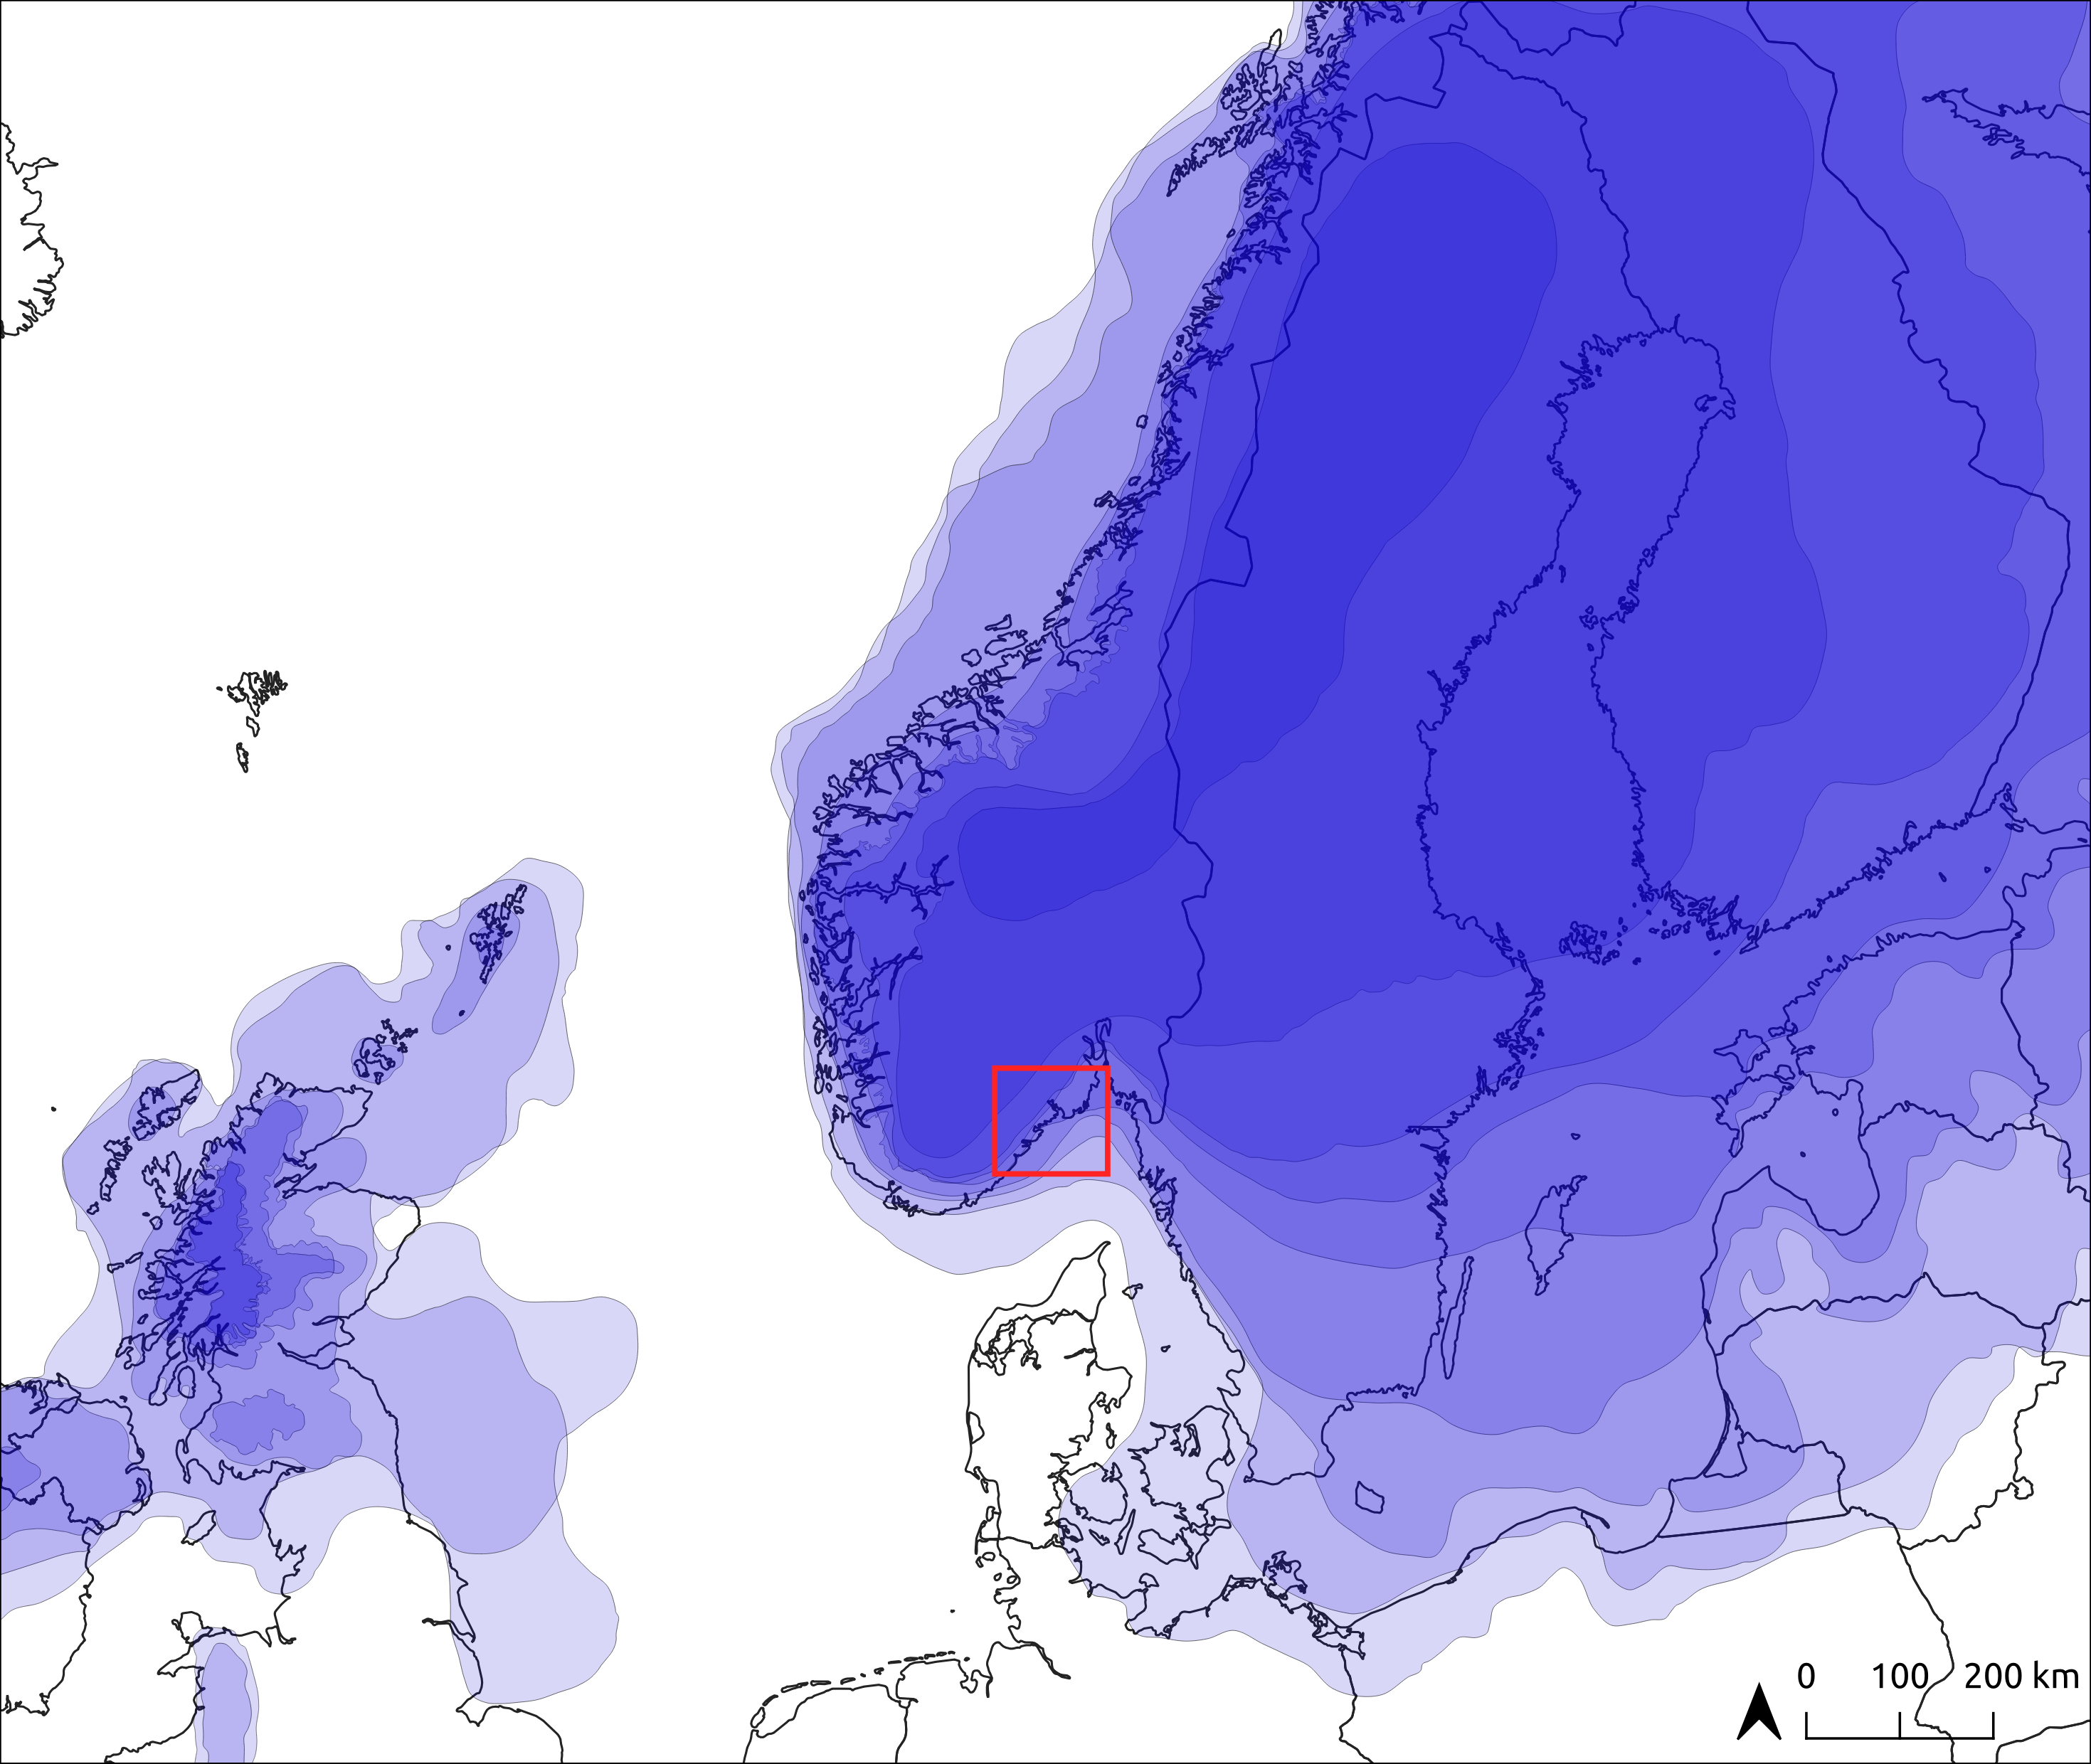
\includegraphics[width=525px]{/home/isak/phd/assessing.sealevel.dating/analysis/figures/deglaciation} 

}

\caption{Deglaciation at 1000 year intervals from c. 17--8 kyr BCE. The study area defined later in the text is marked with a red outline (deglaciation data from Hughes et al. 2016, but see also Romundset et al. 2019 in relation to the study area).}\label{fig:deglaciation}
\end{figure}

The method of shoreline dating has been met with scepticism as related to the fundamental premise that most sites would have been consistently shore-bound, been characterised as a relative dating method for sites located at different elevations within a constrained geographical area, or been argued to offer no more than an earliest possible date for when a site could have been in use (see review by Nordqvist 1999). The most common application in Norway has arguably been to use shoreline dating to provide an approximate date for the occupation of the sites, often in combination with other dating methods (see for example chapters in Jaksland 2014; Melvold and Persson 2014; Reitan and Persson 2014; Reitan and Sundström 2018; Solheim 2017 and below). Recently the method has also been used independently to date a larger number sites to get a general impression of site frequency over time. This is done by aggregating point estimates of shoreline dates in 100, 200 or 500 year bins (Breivik 2014; Breivik and Bjerck 2018; Fossum 2020; Mjærum 2022; Nielsen 2021; Solheim and Persson 2018; see also Jørgensen et al. 2020; Tallavaara and Pesonen 2020). In his review, Nordqvist (1999) argues that there can be little doubt concerning the general applicability of the method -- what is less clear is the level of reliability and chronological resolution that it can offer (see also Johansen 1963).

The shore-bound settlement location of prehistoric hunter-fisher-gatherers in Norway is generally believed to follow both from the exploitation of aquatic resources and from movement and communication, which would have been efficient on waterways (Bjerck 1990; Brøgger 1905:166; also discussed in Berg-Hansen 2009; Bergsvik 2009). The same logic has also been extended to the hinter- and inland regions, where sites are to be predominantly located along rivers and lakes (Brøgger 1905:166; Glørstad 2010:57--87; but see also Gundersen 2013; Mjærum 2018; Schülke 2020). This is to take a dramatic turn at the transition to the Late Neolithic, around 2400 BCE, with the introduction of the Neolithic proper (Prescott 2020; Solheim 2021). The introduction of a comprehensive Neolithic cultural package, including a shift to agro-pastoralism and the introduction of the farm is to have led site locations to be more withdrawn from the shoreline (e.g. Bakka and Kaland 1971; Østmo 2008:223; \textbf{prescott2012?}). That is not to say that waterways and aquatic resources were no longer exploited, but rather that these activities would not have been as tightly integrated with settlement and tool-production areas as in preceding periods (Glørstad 2012). At an earlier stage, at the transition to the Early Neolithic (c.~3900 BCE), pottery is introduced to the sites, and there are some indications of an initial uptake of agriculture at some sites in the Oslo fjord region. However, this appears to be small in scale and is believed to be combined with a continued and predominantly hunter-gatherer life-way, possibly followed by a complete de-Neolithisation in the Middle Neolithic (Hinsch 1955; Nielsen et al. 2019; Østmo 1988:225--227). Nielsen (2021) has recently argued that the initial uptake of agriculture in Early Neolithic south-eastern Norway is combined with a more complex settlement pattern, and that a simple foraging/agricultural dichotomy would underplay the variation present in the Early and Middle Neolithic settlement data (see also e.g. Amundsen et al. 2006; Østmo 1988; Solheim 2012:74). Seen in relation to the question of interest here, the empirical expectation for the above outlined development would thus be a predominantly shore-bound settlement in the Mesolithic, possibly followed by a more varied association between sites and the shore-line with the transition to the Early Neolithic around 3900 BCE, and finally a decisive shift with the Late Neolithic c.~2400 BCE.

Based on the generally accepted premise that most pre-Late Neolithic sites in south-eastern Norway located lower than the marine limit were situated on or close to the contemporaneous shoreline, it is common to err on the side of a shore-bound site location unless there is strong evidence to suggest otherwise. This is for example reflected in survey projects, which are often guided by both a digital and mental reconstruction of past sea-levels (e.g. Berg-Hansen 2009; Eskeland 2017). Similarly, following an excavation, if typological indicators in the assemblages correspond with available shoreline displacement curves, a shore-bound site location is often assumed, even if the typologically informed date-span is too wide to decisively verify this. It is also common to combine this with a qualitative consideration of the landscape surrounding the sites, and an evaluation of the degree to which the site location would have been sensible if the site was not shore bound (e.g. Jaksland 2014; Johansen 1963; Nummedal 1923). This can for example pertain to accessibility. If the site is situated on a ledge in a steep and jagged area of the present day landscape it would make intuitive sense that the site was in use when the ocean reached closer to its elevation, as the site would have been accessible by means of watercraft. Although it appears that the arguments for such site locations are sensible and can for the most part be assumed to hold, comprehensive evaluations and attempts at quantification of this tendency are relatively few (see also Ilves and Darmark 2011).

One of the more extensive evaluations of the relationship between archaeological radiocarbon dates and RSL-change was done by Solheim and colleagues (Breivik et al. 2018; Solheim 2020), who compared 102 radiocarbon dates from 33 Mesolithic sites on the western side of the Oslo fjord to the displacement curve for the Larvik area. They found an overlap between the probability density of the radiocarbon dates with the shoreline displacement curve for 86.5\% of the sites. However, where there was a discrepancy, the main occupation of the sites are still believed to have been shore-bound rather than associated with the deviating \textsuperscript{14}C-dates. This is based on typological and technological characteristics of the assemblages. Whether these mismatches represent later shorter visits that are responsible for the younger radiocarbon dates, or whether these dates are entirely erroneous can be difficult to evaluate (e.g. Persson 2008; Schülke 2020). However, this distinction is not deemed critical here, as what is of interest is settlements and tool-production areas as evidenced by artefact inventories or multiple site features. Not remnants of stays as ephemeral to only be discernible by individual features or dubious \textsuperscript{14}C-dates. The evaluation of the relevance of radiocarbon dates to settlement activity will here therefore be entirely dependent on, and follow the discretion of the original excavation reports.

Other previous evaluations of the correspondence between radiocarbon- and RSL-informed dates have typically followed the same structure as that of Breivik et al. (2018), involving a visual inspection of radiocarbon probability density functions plotted against local shoreline displacement curves based on the elevation of the site (e.g. Åkerlund et al. 1995; Åstveit 2018; Solheim 2020; see also Bjerck 2008b; Kleppe 1985; Ramstad 2009). This approach has a couple of limitations. First of all, the displacement curves are sometimes applied directly to larger study areas, with only some studies having taken the variable uplift-rates into account when performing this comparison (e.g. Åstveit 2018; Fossum 2020; Møller 1987; Persson 2008). Secondly, with this method, the wider the uncertainty range associated with either radiocarbon date or displacement curve, the higher the probability that the confidence intervals overlap, and the higher the probability that we conclude in favour of our hypothesis. This thus leads to an inferential framework that favours uncertainty, which is hardly desirable. In statistical terms this follows from the fact that while one cannot conclude that two dates are different if their confidence intervals overlap, this does not necessarily mean that they are the same. The question thus necessitates a flip from a null-hypothesis of no significant difference, to one of equivalence (e.g. Lakens et al. 2018), as the question of interest is effectively one of synchroneity between events (cf. Parnell et al. 2008). Another limitation of this often-employed method is that it only takes into account the vertical distance between the sites and the sea-level. While this is the main parameter of interest for shoreline dating, the practical implications of a vertical difference in RSL will be highly dependent on local topography and bathymetry. RSL-change can have more dramatic consequences in a landscape characterised by a low relief, as the horizontal displacement of the shoreline will be greater. Taking the spatial nature of the relationship between site and shoreline into account will consequently help get more directly at the behavioural dimension of this relation, and help move the analysis beyond a purely instrumental consideration of the applicability of shoreline dating.

\hypertarget{data}{%
\section{Data}\label{data}}

To get at the relationship between sites and the contemporaneous shoreline, this analysis was dependent on a study area with good control of the trajectory of prehistoric shoreline displacement. While there is displacement data available for other areas of south-eastern Norway (e.g. Hafsten 1957; Sørensen 1979, 1999; and recent compilation by Creel et al. 2022), considerable methodological developments in recent years means that the most well-established displacement curves are from the region stretching from Horten county in the north-east, to Arendal in the south-west. This area has newly compiled displacement curves for Horten (\textbf{romundset2021?}), Larvik (Sørensen et al. in prep; Sørensen, Henningsmoen, et al. 2014; Sørensen, Høeg, et al. 2014), Tvedestrand (Romundset 2018; Romundset et al. 2018), and Arendal (Romundset 2018).

The employed shoreline displacement data is based on the so-called isolation basin method (e.g. Kjemperud 1986; Romundset et al. 2011), which involves extracting cores from a series of basins situated on bedrock at different elevations beneath the marine limit, and dating the transition from marine to lacustrine sediments. Each basin thus represent a high precision sea-level index point (SLIP) which are combined using what has been termed the isobase method to devise a continuous time series for RSL-change, projected to a common isobase (see Creel et al. 2022:5). Furthermore, to minimise the impact of variable uplift rates, the basins are located in a as constrained area of the landscape as possible. Following from the morphology of the retreating ice sheet, the uplift is more severe towards the north-east, meaning that this needs to be adjusted for in the case that any basins are located any significant distance from the common isobase perpendicular to this gradient (Figure \ref{fig:map-iso}). The SLIPs indicate the isolation of the basins from the highest astronomical tide, which is adjusted to mean sea-level in the compilation of the displacement curves based on the present day tidal range. This is assumed to have been the same throughout the Holocene (Sørensen, Henningsmoen, et al. 2014:44). The highest astronomical tide in the study area reaches around 30cm above mean sea-level (Norwegian Mapping Authority 2021:30cm at the standard port Helgeroa in Larvik). Furthermore, the confidence bands of the displacement curves and their trajectory are quite complex constructs, and are the integrated result of both expert knowledge and more objectively quantifiable parameters. The reason for this is in part that the curves do not only contain uncertainty as related to radiometric dates, which are well defined, but also hold potential error as related to the interpretation and analysis of sediment cores, the nature and condition of the basin outlets and the adjustment to a common isobase, to name but a few (e.g. Romundset et al. 2011, 2019; for an alternative approach see Creel et al. 2022). For more details and evaluations done for the compilation of each curve, the reader is therefore referred to the individual publications.

The archaeological data compiled for the analysis consists of excavated Stone Age sites with available spatial data from the coastal region between Horten county in the north-east, to Arendal in the south-west (Figure \ref{fig:map-iso}). These number 155 sites. Of these, 91 sites are associated with a total of 547 radiocarbon dates. Of these, in turn, 67 sites are related to the 259 radiocarbon dates that fall within the Stone Age (9500--1700 BCE), with 95\% probability. These sites and \textsuperscript{14}C-dates form the basis for the analysis. Spatial data in the form of site limits and features, as defined by the excavating archaeologists, were retrieved from local databases at the Museum of Cultural History---the institution responsible for archaeological excavations in the region. In the compiled dataset, each radiocarbon date has been associated with the site features or excavation unit from where they originate, or, where these weren't available, the spatial limit of the entire site. Due to somewhat variable practices between excavations, what available spatial geometry best represents the site limit was decided based on an evaluation of the excavation reports. This means that the limits are variably given as that defined during initial survey, area de-turfed before excavation, area stripped with excavator following the excavation, manually excavated area, or convex hull polygons generated around the site features.

Three of the sites have been associated with agriculture, either directly or in the form building structures. The first is Nordby 1 at which the \textsuperscript{14}C-dates are associated with a Late Neolithic long-house (Gjerpe and Bukkemoen 2008). The Middle Neolithic phase at Kvastad A2 (Stokke and Reitan 2018) and Late Neolithic phase at Nauen A (Persson 2008) are both directly related to farming acitivities. Both of these sites also have radiocarbon dates and lithic inventory associated with Mesolithic forager activities. Following from the expected deviance from the settlement patterns that are to characterise forager sites, these agricultural phases are highlighted in the analysis below. Finally, Nielsen (2021) has recently suggested that Early and Middle Neolithic features from the otherwise younger sites Bratsberg (Wenn 2012) and Larønningen (Røberg 2012) could be related to early agricultural activity in the Oslo fjord region. Due to the uncertain and somewhat speculative nature of this suggestion, these are omitted here.

The elevation data used for the analysis is a digital terrain model (DTM) freely available from the Norwegian Mapping Authority (Norwegian Mapping Authority 2018, \url{https://hoydedata.no}). It was here opted for the 10m resolution DTM rather than the higher-resolution 1m version. In addition to resulting in considerably less processing time, the higher resolution elevation model is more vulnerable to smaller-scale modern disturbances that the 10m version is not impacted by. The 10m resolution DTM of the study area is a down-sampled version of the 1m version and has a height accuracy with a systematic error of 0.1m (Norwegian Mapping Authority 2018). All data and R programming code (R Core Team 2021) required to run the analyses, as well as the derived data are freely available in an online repository at \url{https://osf.io/7f9su/}, organised as a digital research compendium following Marwick et al. (2018).

\begin{figure}

{\centering 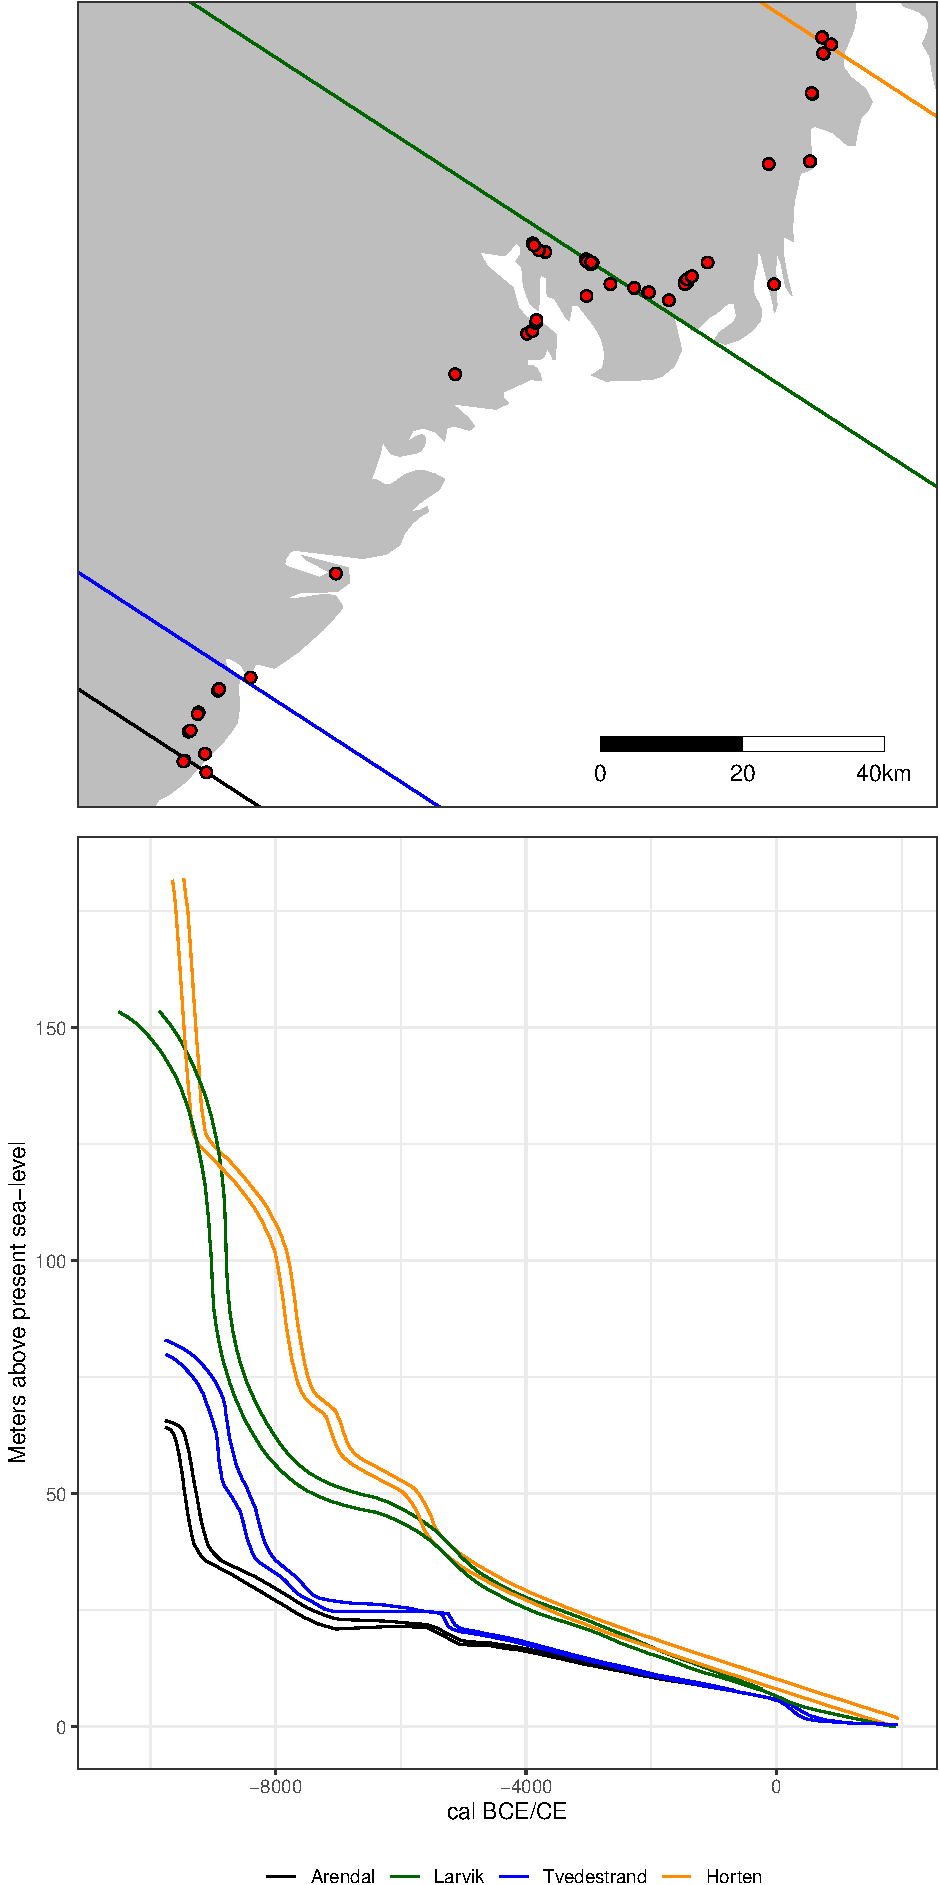
\includegraphics{../figures/map-iso-1} 

}

\caption{A) Distribution of the  67  analysed sites relative to the isobases of the displacement curves. The isobases have a direction of 327$^{\circ}$ (Romundset et al. 2018), B) Displacement curves. Note the increasing steepness of the curves towards the north-east.}\label{fig:map-iso}
\end{figure}

\hypertarget{methods}{%
\section{Methods}\label{methods}}

The method of shoreline dating is based on the spatial relationship between two phenomena, occupation of sites and shoreline displacement, each associated with their own range of temporal uncertainty. The first task was therefore to ascribe likely date ranges and associated uncertainty to these dimensions. To take account of the gradient in the isostatic rebound, the trajectory of shoreline displacement was first interpolated to each site location based on the distance to the isobases of the displacement curves using inverse distance weighting (e.g. Conolly 2020; Conolly and Lake 2006:94--97). This was done for each year along the entirety of the curves, weighting the interpolation by the standard squared inverse of the distances. The result of this process is shown for an example site in Figure \ref{fig:example-1}. For the date ranges associated with the sites, all radiocarbon dates were first individually calibrated using the IntCal20 calibration curve (Reimer et al. 2020) using OxCal v4.4.4 (Bronk Ramsey 2009) through the oxcAAR package for R (Hinz et al. 2021). Radiocarbon dates associated with each site were then grouped if they overlapped with 99.7\% probability, meaning these were effectively taken to represent the same event, here termed settlement or site phases. In the case where there are multiple dates believed to belong to a single settlement phase, these were modelled using the Boundary function in OxCal and then summed. Multiple phases at a single site were treated as independent of each other.

The excavation of archaeological sites typically follow from residential and commercial development, as well as the expansion of infrastructure. As the data collection for the DTM was started by the Norwegian Mapping Authority in 2016, the area of the DTM immediately surrounding the sites has therefore sometimes been severely impacted by disturbances after the excavation of the site. In addition to employing 10m resolution DTM to alleviate some of these issues, this also necessitated some additional editing of the elevation raster. This involved manually defining the extent of problem areas such as railways, highways, quarries and the like. The DTM values on these were then set to missing, and new elevation values were interpolated from the surrounding terrain. This was done using regularised spline interpolation with tension (e.g. Conolly 2020), using the default settings of r.fillnulls from GRASS GIS (GRASS Development Team 2017) in R through the package rgrass7 (Bivand 2021). In addition to code and original spatial data being available in the digital research compendium for this paper, the analysis of each individual site is presented in the supplementary material where it has been noted when the area surrounding a site has been edited in this manner.

Armed with a likely date range for the occupation(s) of each site, an estimated trajectory of relative sea-level change at that location, and a DTM edited to remove substantial modern disturbances, the simulations were performed. A single simulation run involved first drawing a single year from the posterior density estimate of a given occupation phase of a site (Figure \ref{fig:example-2}). This year then has a corresponding likely elevation range for the contemporaneous shoreline from which an elevation value was drawn uniformly, using intervals of 5cm. The sea-level was then raised to this elevation on the DTM by defining all elevation values at or below this altitude as missing. Polygons were then created from the resulting areas with missing values. The horizontal distance was then found by measuring the shortest distance between site and sea polygons, and the vertical distance by subtracting the elevation of the sea-level from the lowest elevation of the site polygon. The topographic distance between site and sea was also found by measuring the distance while taking into account the slope of the terrain on the DTM. This was done using the topoDistance package for R (Wang 2019). The topographic distance was measured between the site polygon and the horizontally closest point on the shoreline. This means that the distance is not necessarily measured as the closest topographic distance to the shoreline, but rather as the shortest topographic path to the horizontally closest point on the shoreline. Not finding the topographically closest point significantly reduced the computational cost of the analysis, and is deemed unlikely to have a considerable impact on the results given the distances considered. The shortest topographic path was found using the Moore neighbourhood of eight cells (e.g. Conolly and Lake 2006:253; Herzog 2013). In the case where the sea-polygons intersects the site polygon, all distance measures were set to zero. In the case that the sea-polygons completely contain the site, the horizontal and topographic distance measures were made negative, and the vertical distance was instead measured to the highest point on the site polygon. While it is safe to assume that an archaeological site was not occupied when it was located beneath sea-level, a negative result can reflect the inherent uncertainty in this procedure, and might also help identify discrepancies in displacement data or radiocarbon dates. Negative values were therefore retained with the exception of for the sites Gunnarsrød 5 and Pjonkerød R1, where the negative values are believed to result from modern disturbances in the DTM rather than the \textsuperscript{14}C-dates or displacement curves (see supplementary material for more details).

This process was repeated 1000 times for each phase for each site. The choice of 1000 simulation runs follows from an evaluation of when the mean distances between site and shoreline converged when running 5000 iterations of the simulation on the site Hovland 5, available in the supplementary material (cf. Crema et al. 2010:1125). Hovland 5 was chosen for this evaluation as it has a fairly imprecise date and is located in area of quite complex topography.

\begin{figure}

{\centering 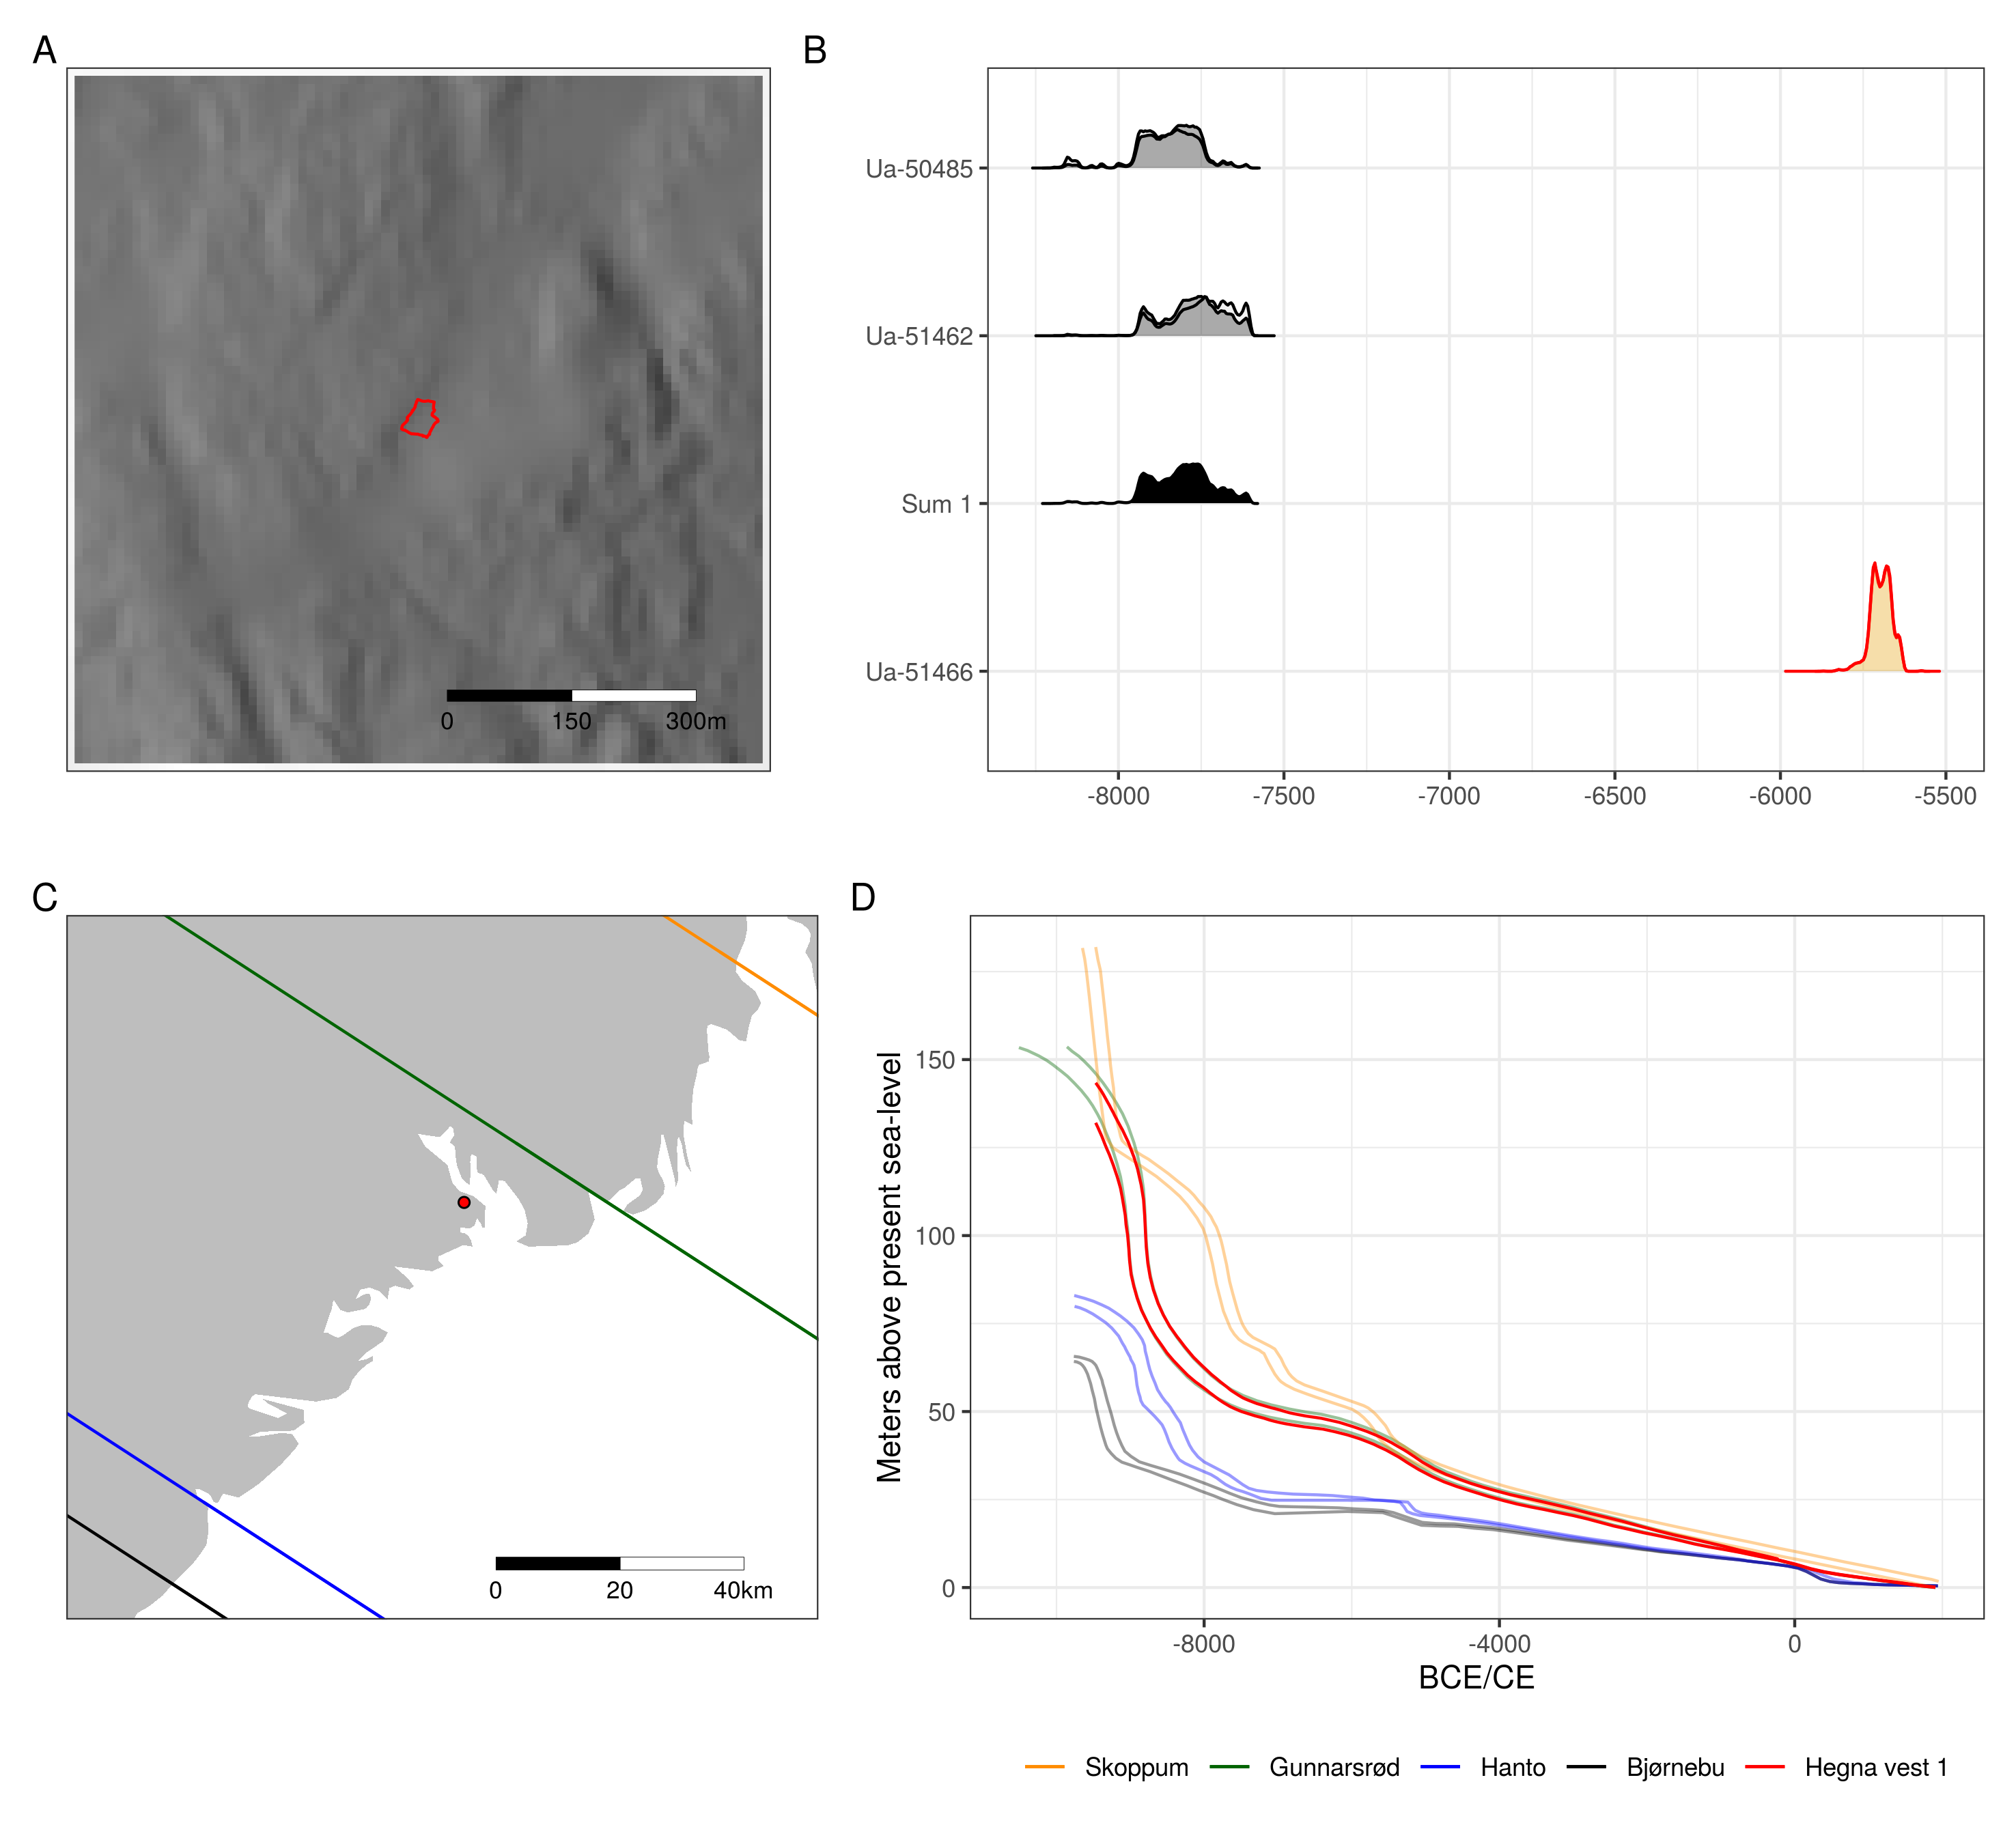
\includegraphics[width=500px]{/home/isak/phd/assessing.sealevel.dating/analysis/figures/example_map} 

}

\caption{Example site Hegna vest 1 (Fossum 2017). A) Location of the site on the edited 10m resolution DTM. The red outline is the site limit. B) Radiocarbon dates associated with the site. Fill colour indicates what dates are assumed to belong to the same settlement phase. Multiple dates are modelled using the Boundary function in OxCal and then summed. The red outline indicates that the date does not match the typological indicators in the artefact assemblage of the site. C) The location of the site within the study area relative to isobases of the employed displacement curves. D) Displacement curve interpolated to the site location.}\label{fig:example-1}
\end{figure}

\begin{figure}

{\centering 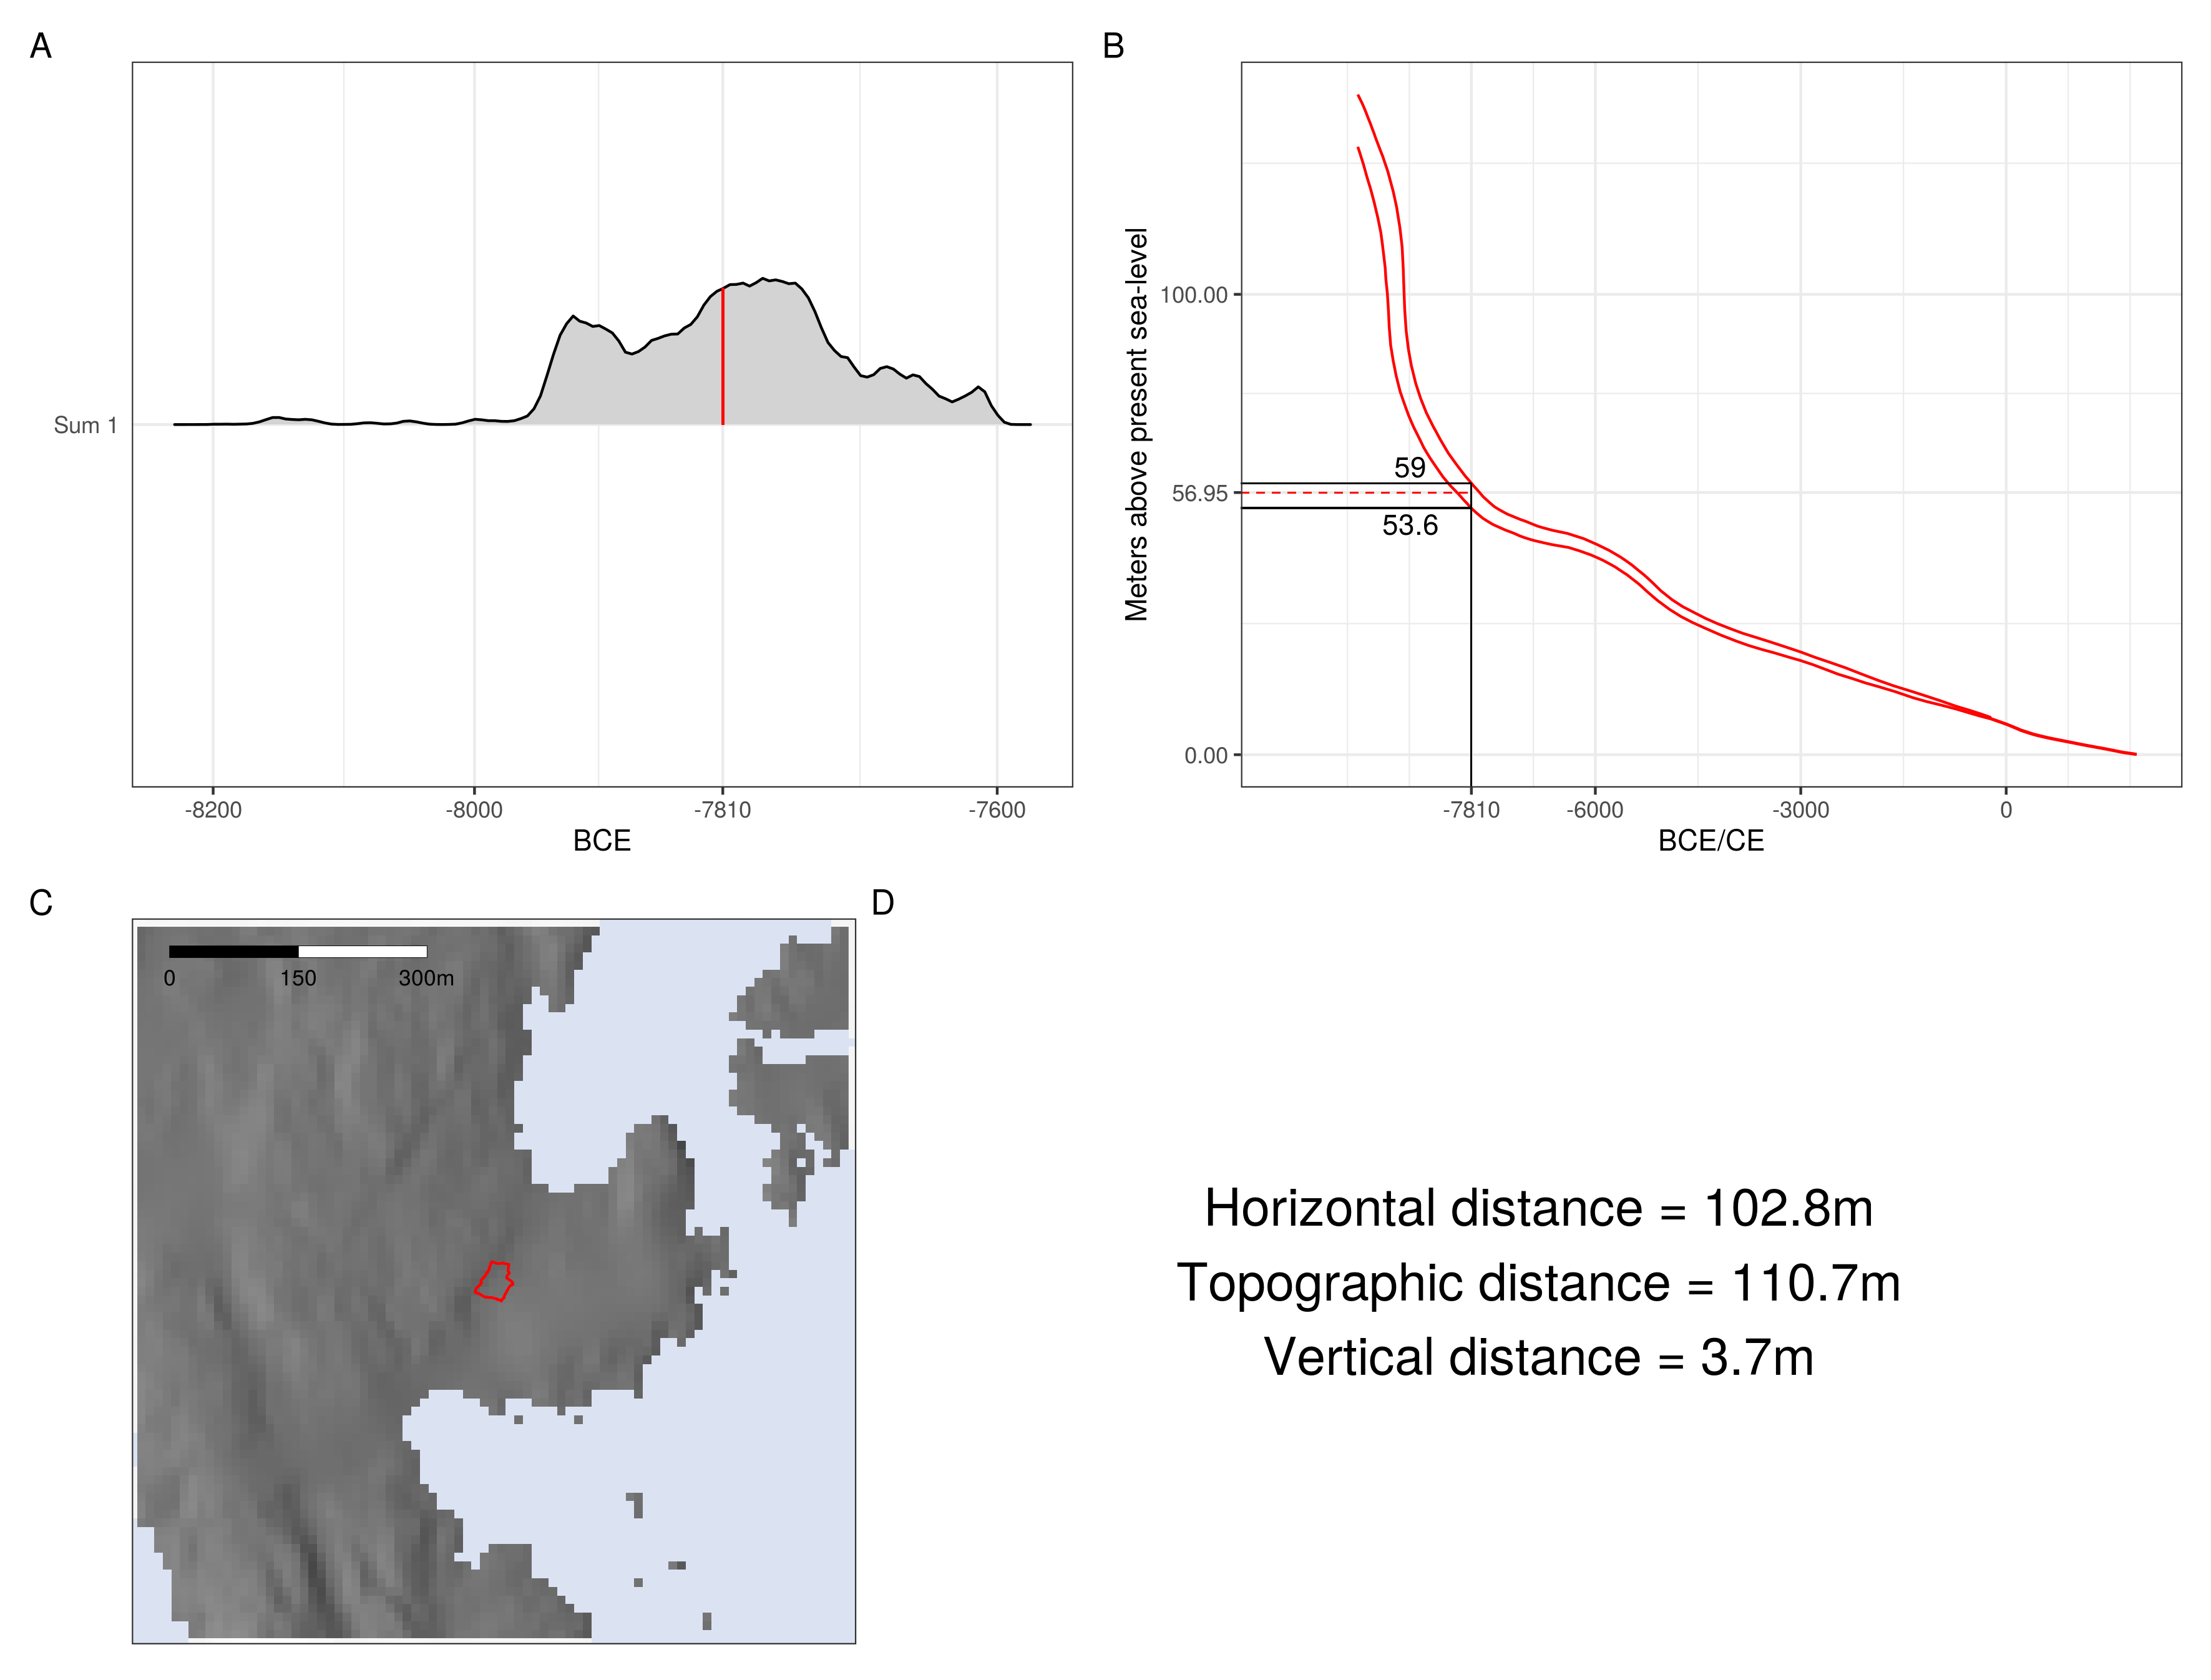
\includegraphics[width=500px]{/home/isak/phd/assessing.sealevel.dating/analysis/figures/example_sim_map} 

}

\caption{Example of a single simulation run on the site Hegna vest 1. A) The simulation starts by drawing a single year from the posterior density esimate.  B) This then corresponds to an elevation range on the interpolated displacement curve. A single elevation is drawn uniformly from this range using 5cm intervals. C) The sea-level is then adjusted on the DTM to this elevation and the various distance mesaures are found. D) The numerical result of the simulation run.}\label{fig:example-2}
\end{figure}

\begin{figure}

{\centering 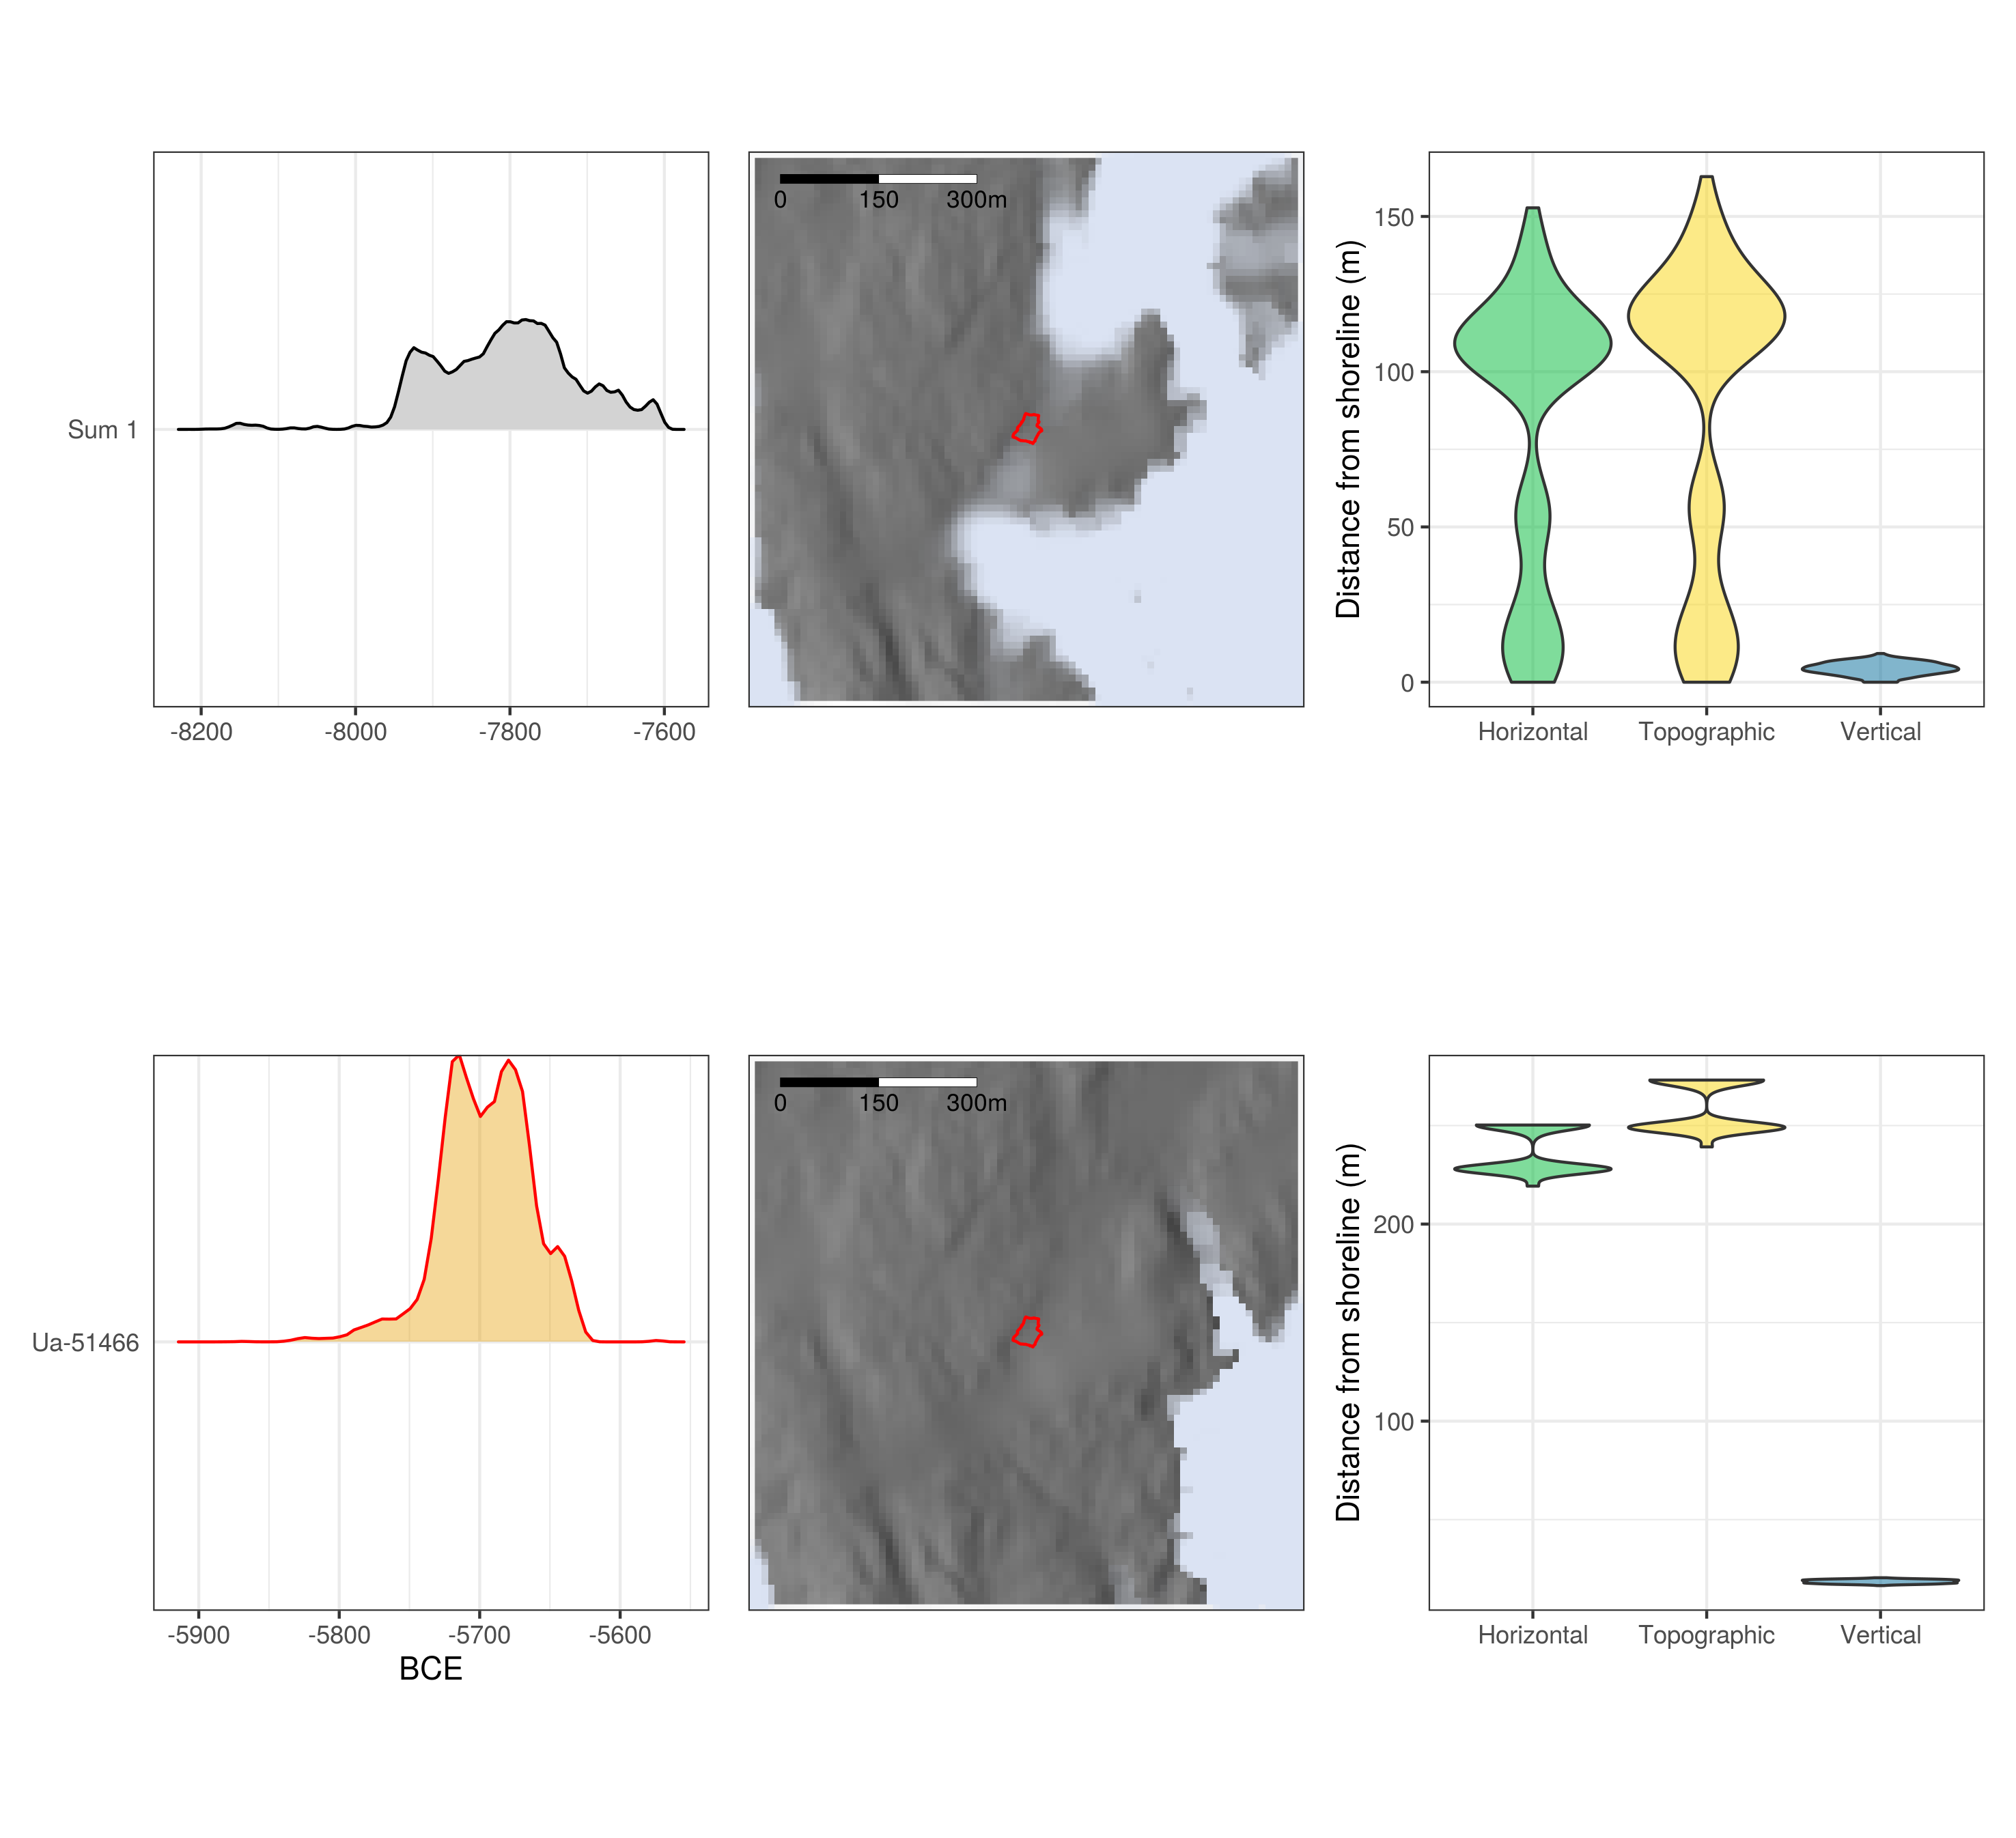
\includegraphics[width=500px]{/home/isak/phd/assessing.sealevel.dating/analysis/figures/example_sim_result} 

}

\caption{The result of 1000 simulation runs for each of the two groups of dates on the site Hegna vest 1. The first column of plots shows the radiocarbon probability density function from where dates were drawn during simulation. The second column displays the result of simulating the raised sea-level 1000 times. The more opaque the colour, the more times the sea-level was simulated to that location. The third column shows violin plots of the different distance measures across all simulations.}\label{fig:example-3}
\end{figure}

\hypertarget{simulation-results}{%
\section{Simulation results}\label{simulation-results}}

Overall, as is indicated by the measures for central tendency and the almost solid line along the 0m mark on the y-axes, the simulations show that the sites tend to have been situated close to the shoreline when they were in use (Figure \ref{fig:results}). Some of the sites are situated considerable distances from the shoreline when the dates believed to be erroneous in the original reports are included (Figure \ref{fig:results}A), but if one accepts the interpretation that these do not date the main occupation of the sites, as is indicated by the artefact inventories, Figure \ref{fig:results}B gives considerable support to the notion that the sites were in use when they were situated on or close to the contemporaneous shoreline. The distances for some of the earliest sites appears somewhat high, but this can likely be explained as the result of the steepness of the displacement curves for the earliest part of the Holocene (Figure \ref{fig:map-iso}B), which leads the uncertainty of the \textsuperscript{14}C-dates to give a wider possible elevation range for the simulated sea-level. Another immediately striking result is the apparent deviation from the shoreline towards the end of the Stone Age. From around 2500 BCE several sites are situated a considerable distance from the shoreline, and while a couple remain horizontally and topographically close, most appear to be elevated a considerable distance from the sea-level, as indicated on the plot for vertical distance. There are also a couple of sites located some distance from the shoreline just after 4000 BCE. While the sample size is limited, this would thus be in line with a development that sees an increase in settlements located in the immediate inland around this time.

The negative values around 8000 BCE originate from the sites Løvås 1, 2 and 3. These are recently excavated, well-dated sites situated in a relatively undisturbed area of the landscape. While there would be a danger of circularity of having archaeological sites inform a reconstruction RSL-change, and in turn use these to evaluate the degree of shore-bound settlement, the sites do clearly represent a upper limit for the sea-level, as they would not have been in use when located under water. It could therefore seem that the Løvås sites represent a case where the archaeological material indicates a slight discrepancy in the geological reconstruction of shoreline displacement in the area.

Accepting that shoreline dating appears to loose utility around the transition to the Late Neolithic, as indicated by the clear deviation in site location from the shoreline after this, the results for from Figure \ref{fig:results}B is given again in Figure \ref{fig:results2}A, excluding all simulation results younger than 2500 BCE. Furthermore, all negative values have here been set to zero, under the assumption that these result from uncertainty or errors in the data, and not actual site locations. The resulting best point estimate for the vertical distance between sites and shoreline for the pre-Late Neolithic is given by the median at 4m, while 95\% of the values fall within the range 0--18m. That is, for 95\% of the cases, the shoreline was simulated to be situated on or down to 18m below the site location. While these values remain the same when only the Mesolithic dates are included (Figure \ref{fig:results2}B), the mean and standard deviation are slightly constrained. Furthermore, while the median for horizontal and topographic distance is only 10m across all plots in Figure \ref{fig:results2}, the variation in the statistics for dispersion is greater, illustrating the point that minor variations in vertical distance can have substantial consequences for these distance measures, depending on the surrounding topography.

\begin{figure}

{\centering 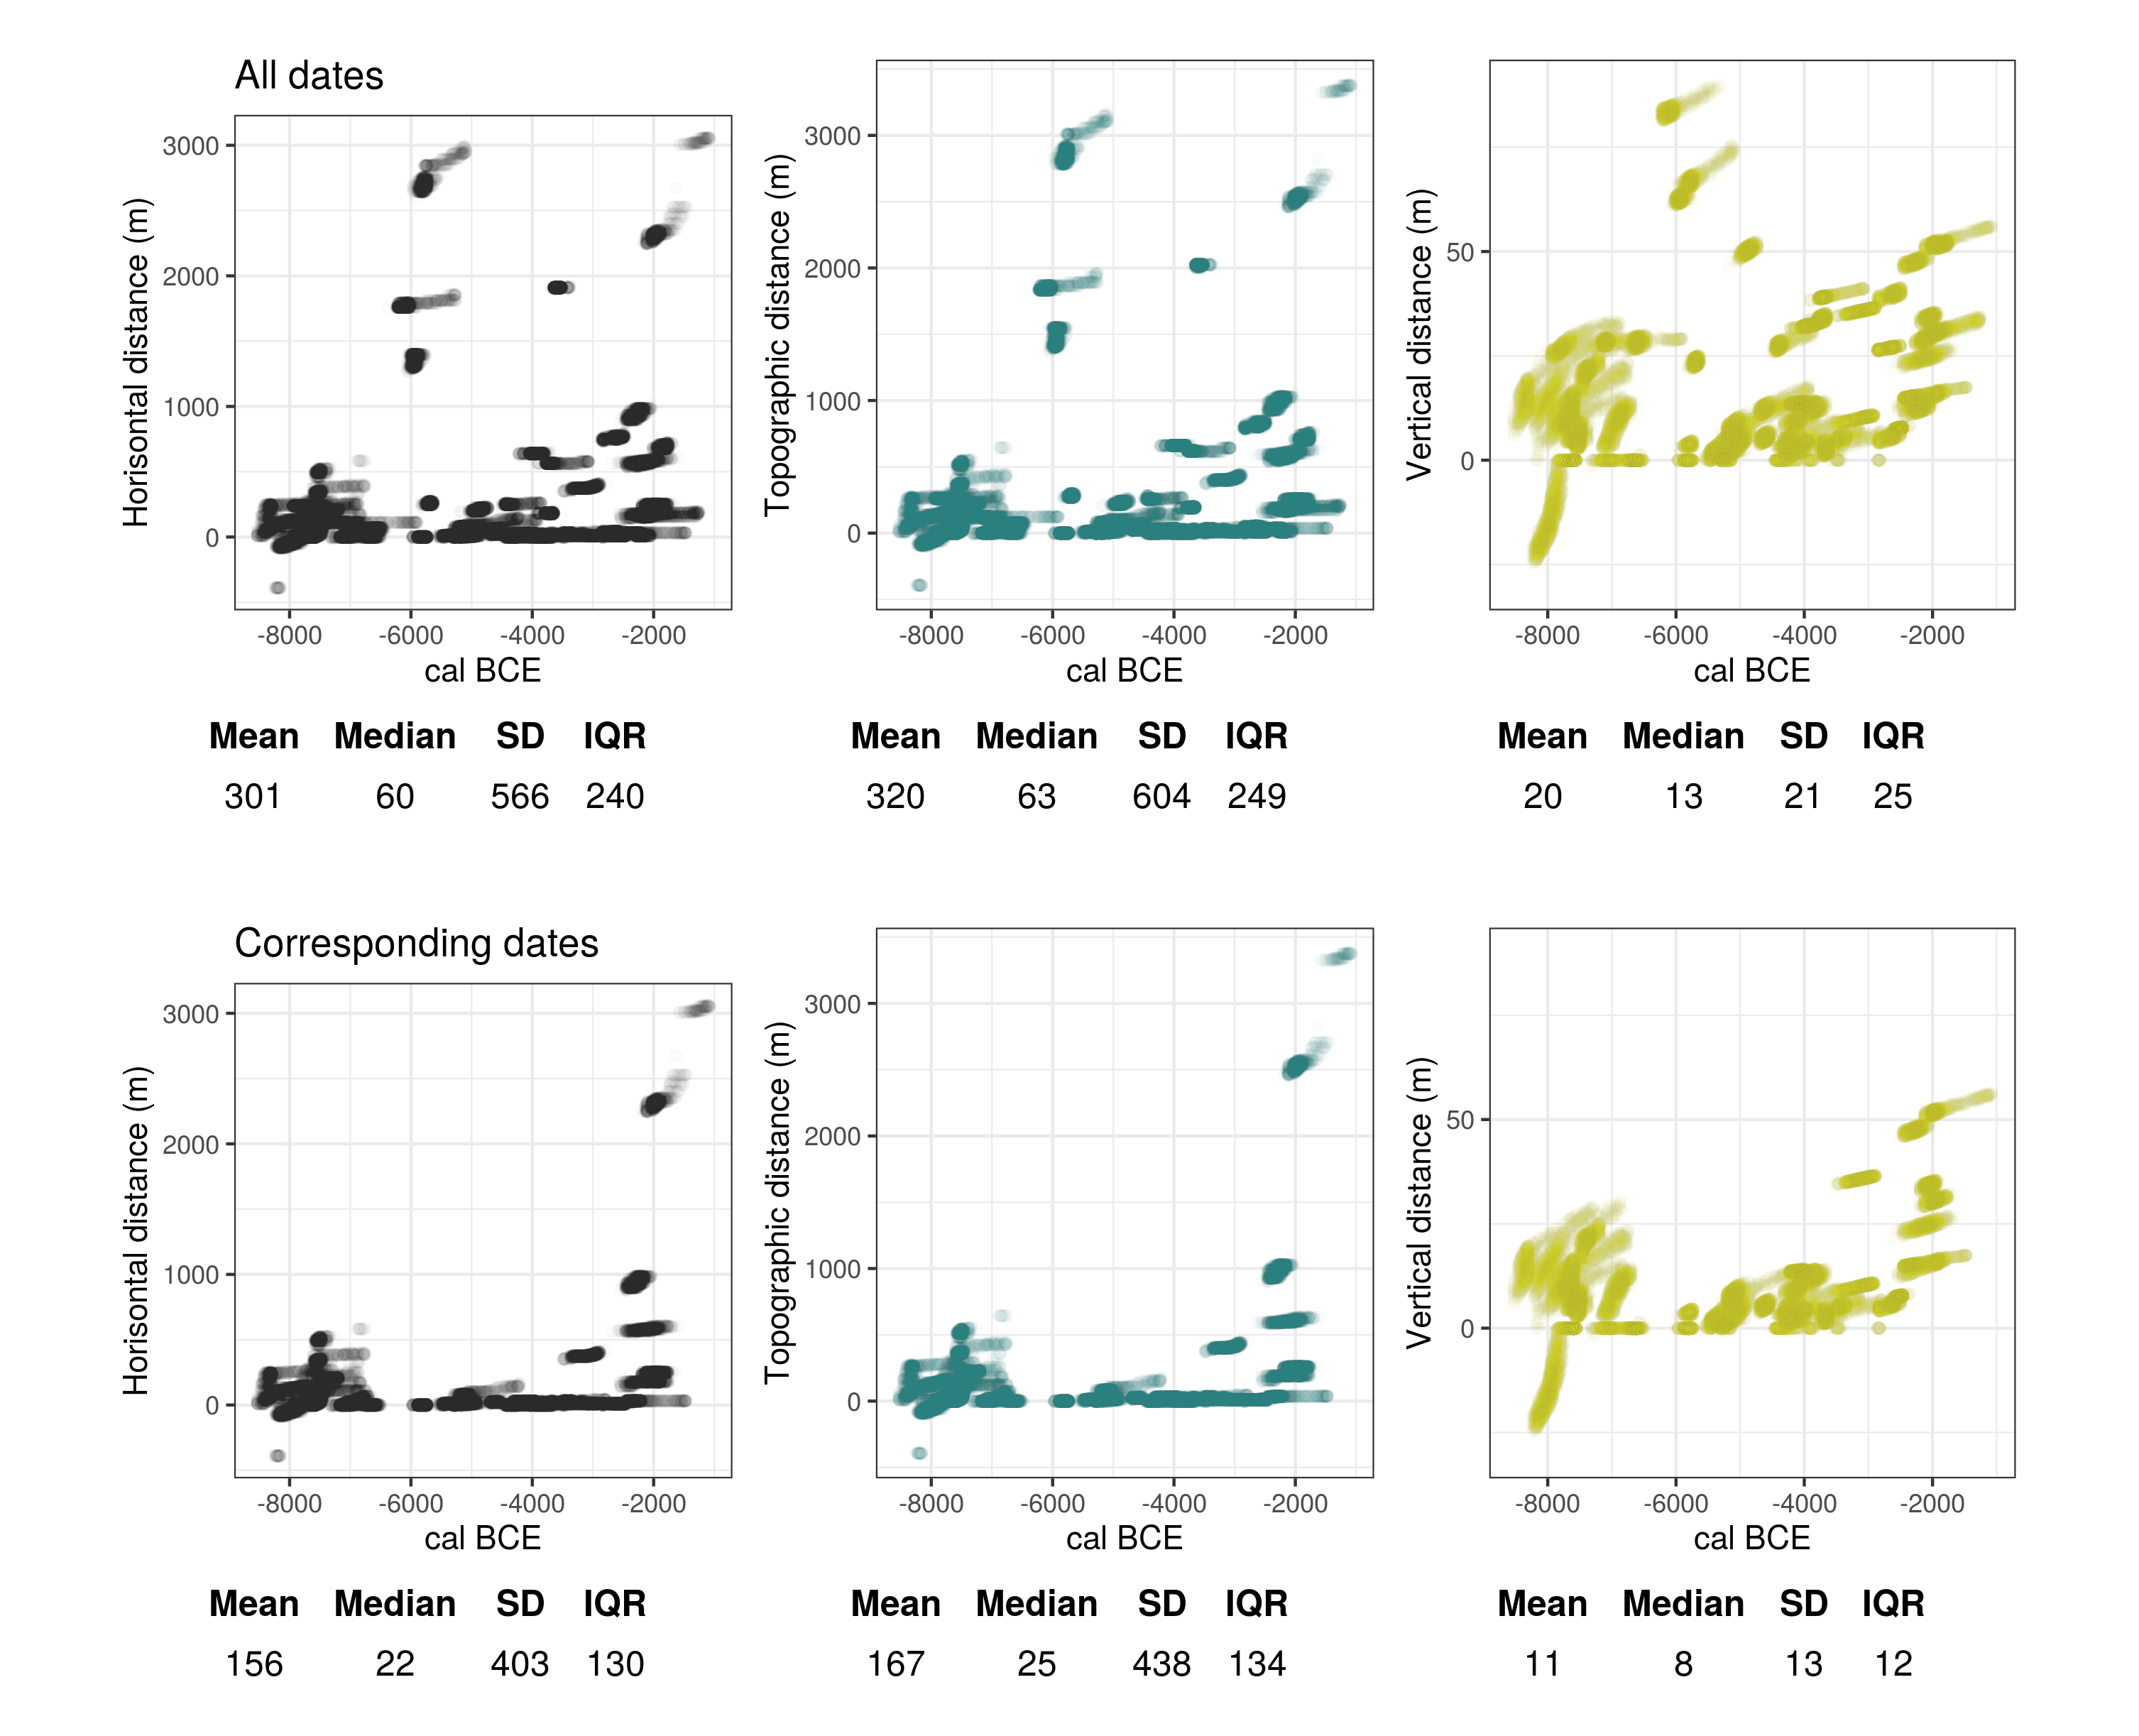
\includegraphics[width=500px]{/home/isak/phd/assessing.sealevel.dating/analysis/figures/results} 

}

\caption{The result of running the analysis across all sites. Each data point is plotted with some transparency, meaning that the more intense the colour, the more often those values occured. Results associated with agricultural acitivites are plotted in grey. The first row A) shows the result of including all dates to the Stone Age, including those seen as otherwise  unrelated to the main occupation of the sites. The second row B) shows the result of excluding these. The table under each plot lists some corresponding statistics for central tendency and dispersion.}\label{fig:results}
\end{figure}

\begin{figure}

{\centering 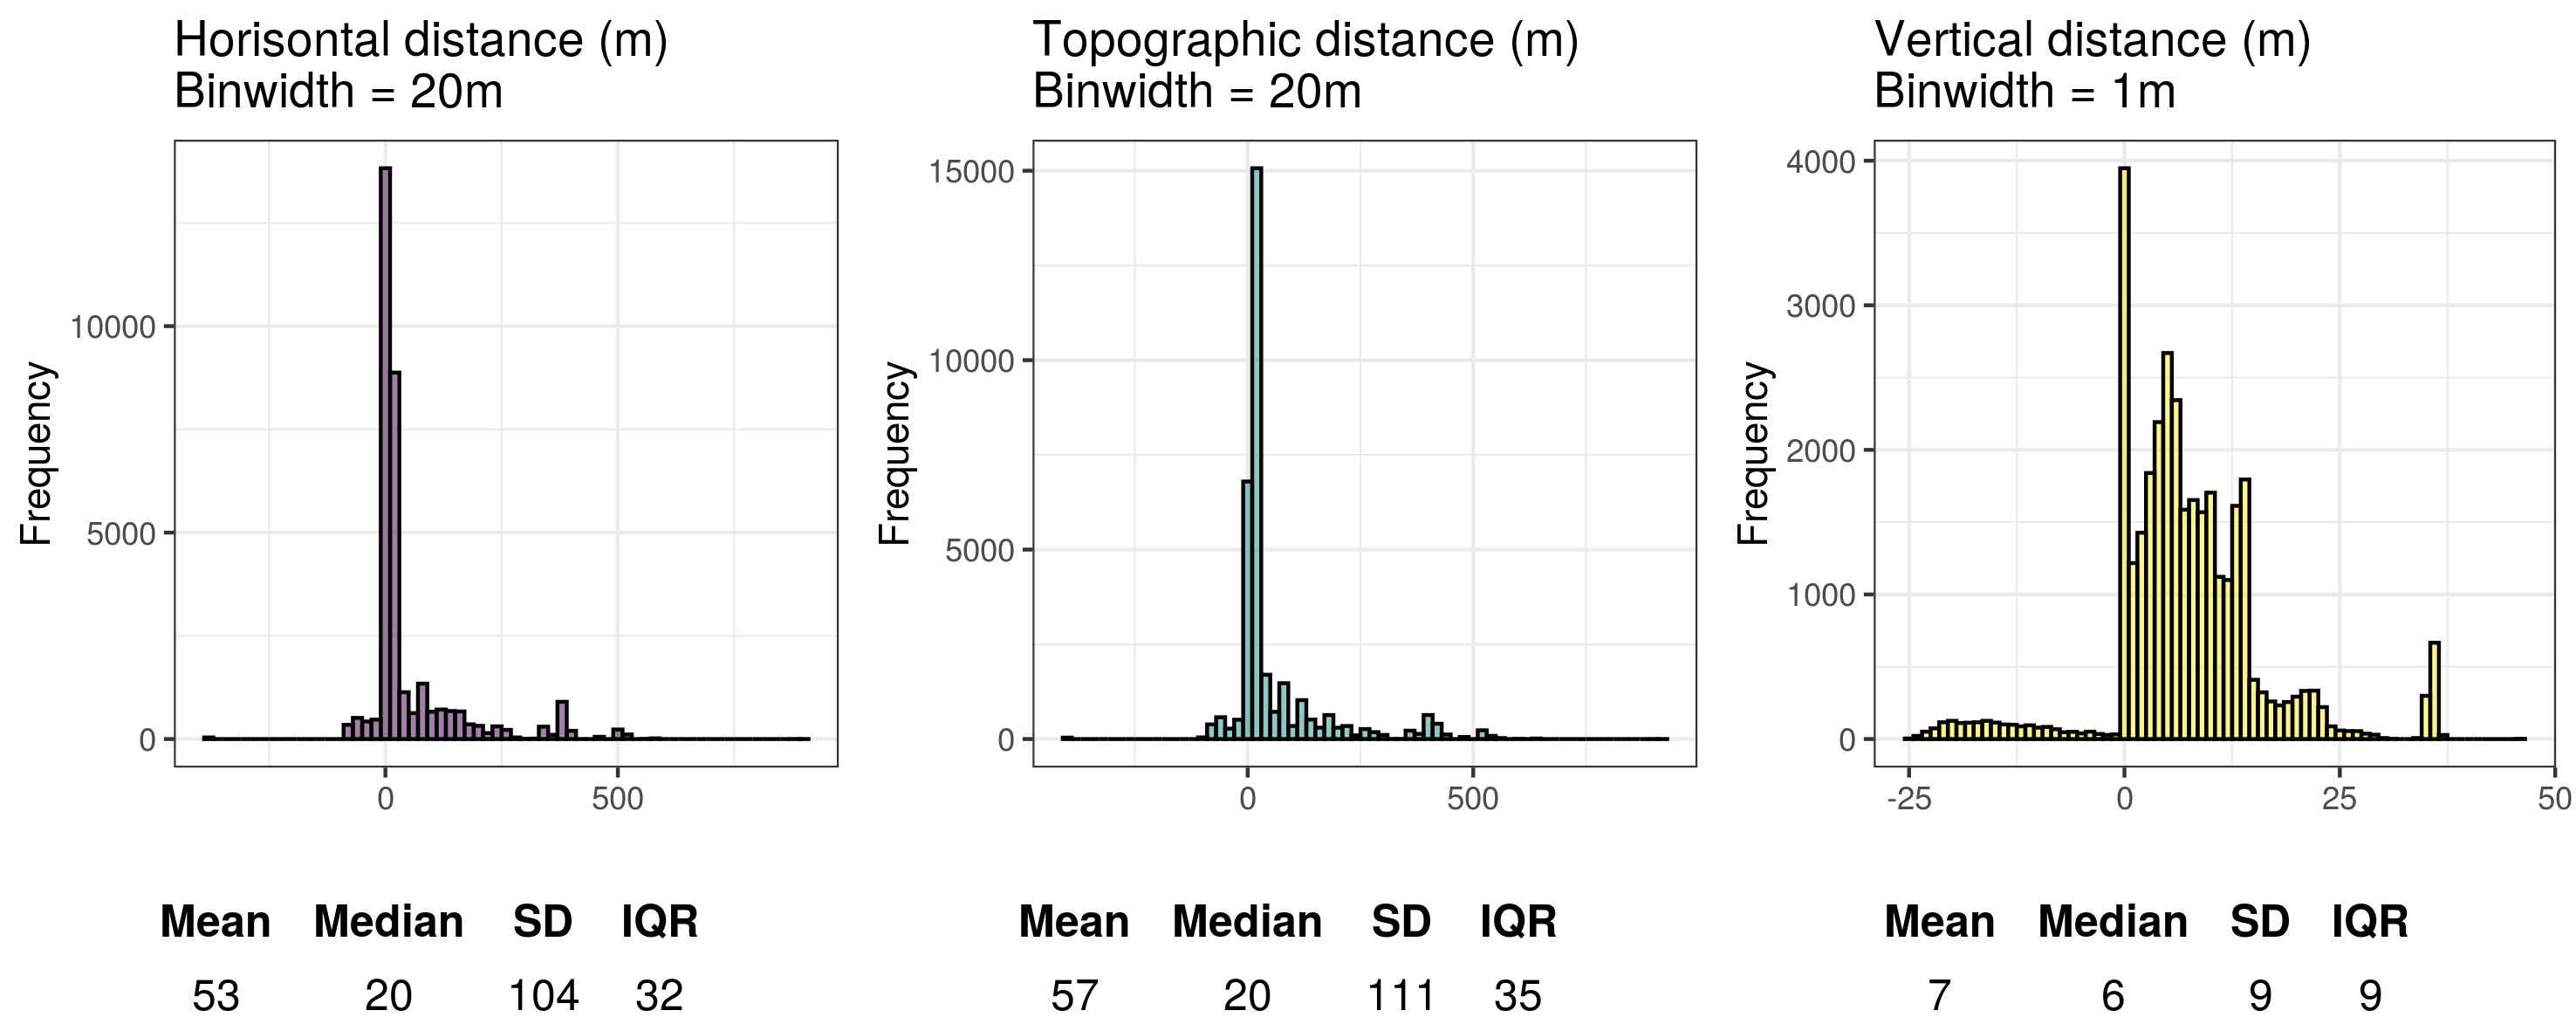
\includegraphics[width=525px]{/home/isak/phd/assessing.sealevel.dating/analysis/figures/results2} 

}

\caption{Histograms showing the simulated distance from the shoreline using dates corresponding to the site inventories. Negative values have been set to zero. A) Simulated results older than 2500 BCE, and B) simulated results older than 4000 BCE.}\label{fig:results2}
\end{figure}

\begin{figure}

{\centering 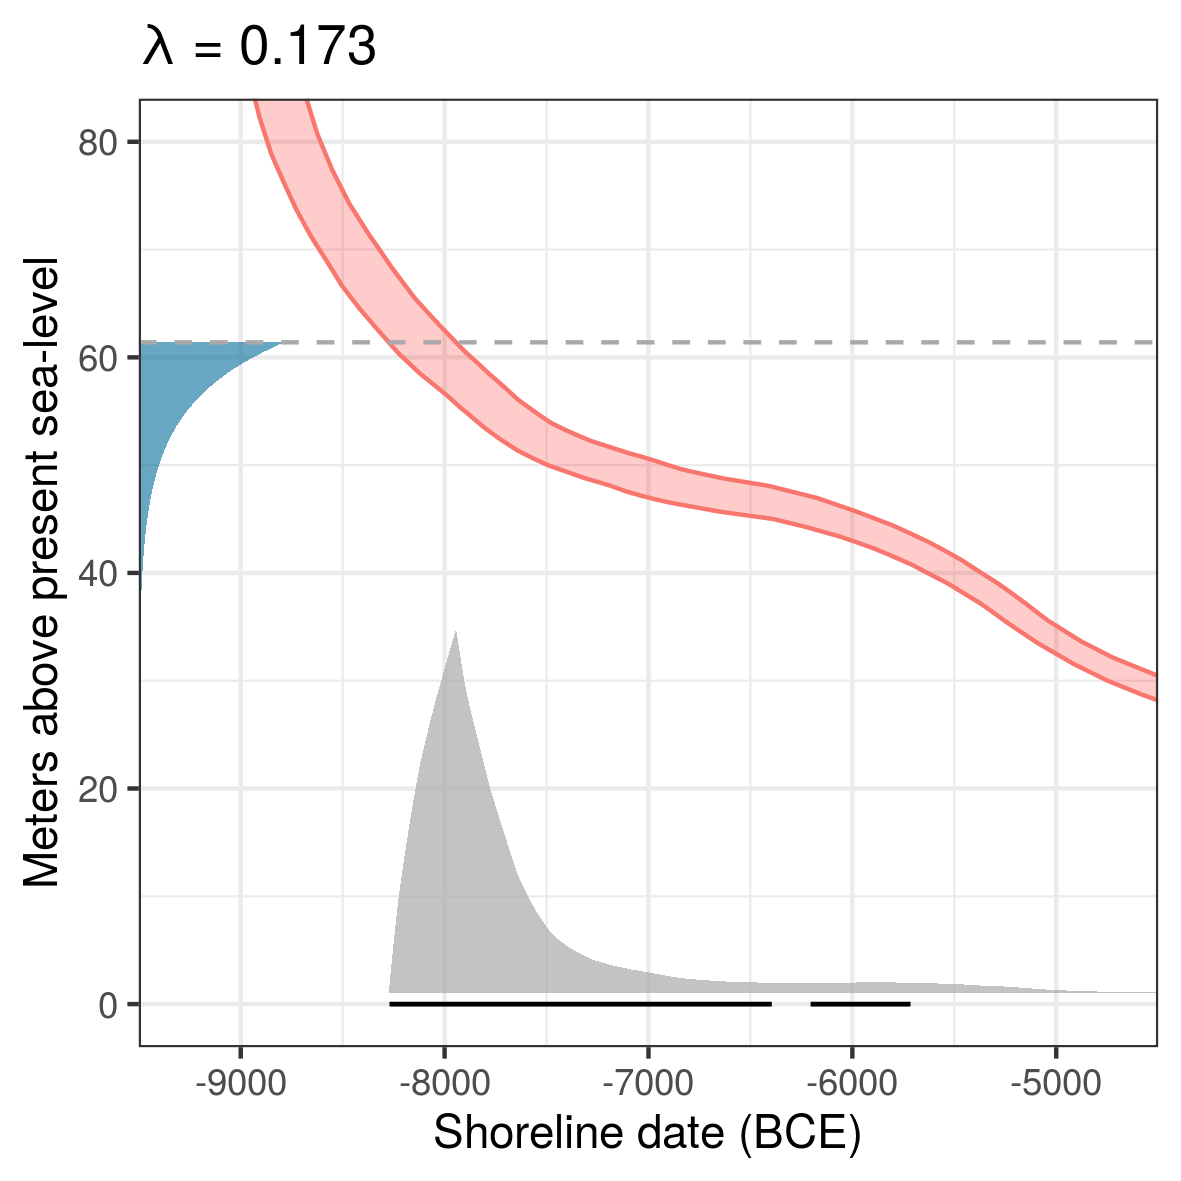
\includegraphics[width=500px]{/home/isak/phd/assessing.sealevel.dating/analysis/figures/sdate} 

}

\caption{Shoreline dating Hegna vest 1. The dashed line indicates the elevation of the site. The decay ratio follows Figure 7A. The shoreline date in grey is underlined with the 95\% HDR in black.}\label{fig:exampledat}
\end{figure}

\hypertarget{shoreline-dating}{%
\section{Shoreline dating}\label{shoreline-dating}}

An exponential function has been fit to the distributions for vertical distance using maximum likelihood estimation (Figure \ref{fig:results2}). While it makes theoretical sense that a process of exponential decay explains this relationship, it is also clear that this does not perfectly match the data. However, this can at least in part be related to methodological factors, where the accumulation of distance-values on the 0m mark likely follow from forcing negative values to zero, from the resolution of the spatial data, and from defining intersecting sea- and site polygon as having a distance of zero. If one accepts this, the probability density function for exponential decay can be used to characterise the vertical distance between sites and the shoreline and leveraged for devising a method for shoreline dating that takes this into account.

The procedure is thus aimed at determining the likely age of the occupation of a site based on its altitude above present day sea-level, with reference to shoreline displacement and the likely elevation of the site above sea-level when it was in use. For simplicity, this is conceptually treated a single event and thus the possibility of multiple or continuous phases of occupation is not treated explicitly. This leads the problem to become analogous to that of the calibration of a radiocarbon date. Drawing on the standard Bayesian formulation for the calibration procedure for 14C-dates (e.g. Bronk Ramsey 2009), the probability density associated with the calendar age can then be given as

\begin{equation} 
  p(x_{i} | \thetha_{i}) ~ p(\theta_{i} | x_{i})p(x_{i})
  \label{eq:bayes}
\end{equation}

where for any site i the unknown calendar date is denoted \(\thetha\) and the elevation of the contemporaneous sea-level \(x\). The elevation of the sea-level is dependent on the present day elevation of the site \(\alpha\) and the distance between site and the shoreline \(d\). Based on the simulation results above, the distance from the elevation of the site to the contemporaneous shoreline is defined by the probability density function for exponential decay

\begin{equation}
  p(d) = \lambda {e}^{- \lambda x}
  \label{eq:decay}
\end{equation}

Where \(\lambda\) is the decay ratio. This can then be coupled with the trajectory of relative sea-level change, denoted RSL, to find the probability density for the calendar date. Here the relative sea-level change is defined by a uniform probability density function over the range between the lower and upper displacement curves interpolated to the site location

\begin{equation}
p(RSL) = U[RSL_{lower}, RSL_{upper}]    
  \label{eq:rsl}
\end{equation}

\begin{equation} 
  placeholder
  \label{eq:shoredate}
\end{equation}

Eq. \eqref{eq:shoredate} is used to shoreline date the same sites from where this relationship was derived (Figure \ref{fig:shoredate}), employing \(\lambda\) = 0.173 for the decay ratio in Eq. \eqref{eq:decay}. This is the ratio identified when considering all of the pre-Late Neolithic simulation results (Figure \ref{fig:results2}A). For illustrative purposes the Late Neolithic sites were also subjected to the proposed method for shoreline dating. Following from having defined the distance between intersecting sea- and site polygons as zero during simulations, the sites were dated using the mean elevation of the site polygons to allow for some variation in elevation over the site limits. The synchroneity between radiocarbon and shoreline dates was then evaluated using the method presented by Parnell et al. (2008). Here, 100,000 age samples drawn from the probability density function of each shoreline date were subtracted from 100,000 age samples drawn from the corresponding modelled \textsuperscript{14}C-dates. The resulting range of the 95\% highest density region (HDR, Hyndman 1996) was then checked to see if it crosses zero, in which case the dates are considered to be in agreement (Figure \ref{fig:shoredatediff}). When excluding the earliest occupation phase at Gunnarsrød 5, the deviation of which is to be expected based on issues with the DTM (see above), the shoreline date correspond to the radiocarbon dates in 58 out of 68 cases (84\%). Only including dates modelled to be older than 2500 BCE with 95\% probability, i.e.~older than the Late Neolithic, improves this to 56 out of 61 cases (92\%). When only including dates older than 4000 BCE with 95\% probability, i.e.~only Mesolithic site phases, the success rate is further increased to 46/49 (94\%). The three failed Mesolithic shoreline dates are from the early sites Langemyr and Kvastad A2, with the likely implication that a lower decay ratio than what is used for characterising the distance between site and shoreline for all sites in aggregate should be used for sites known to be from the earliest part of the Mesolithic (see also Figure \ref{fig:results}).

\begin{figure}

{\centering 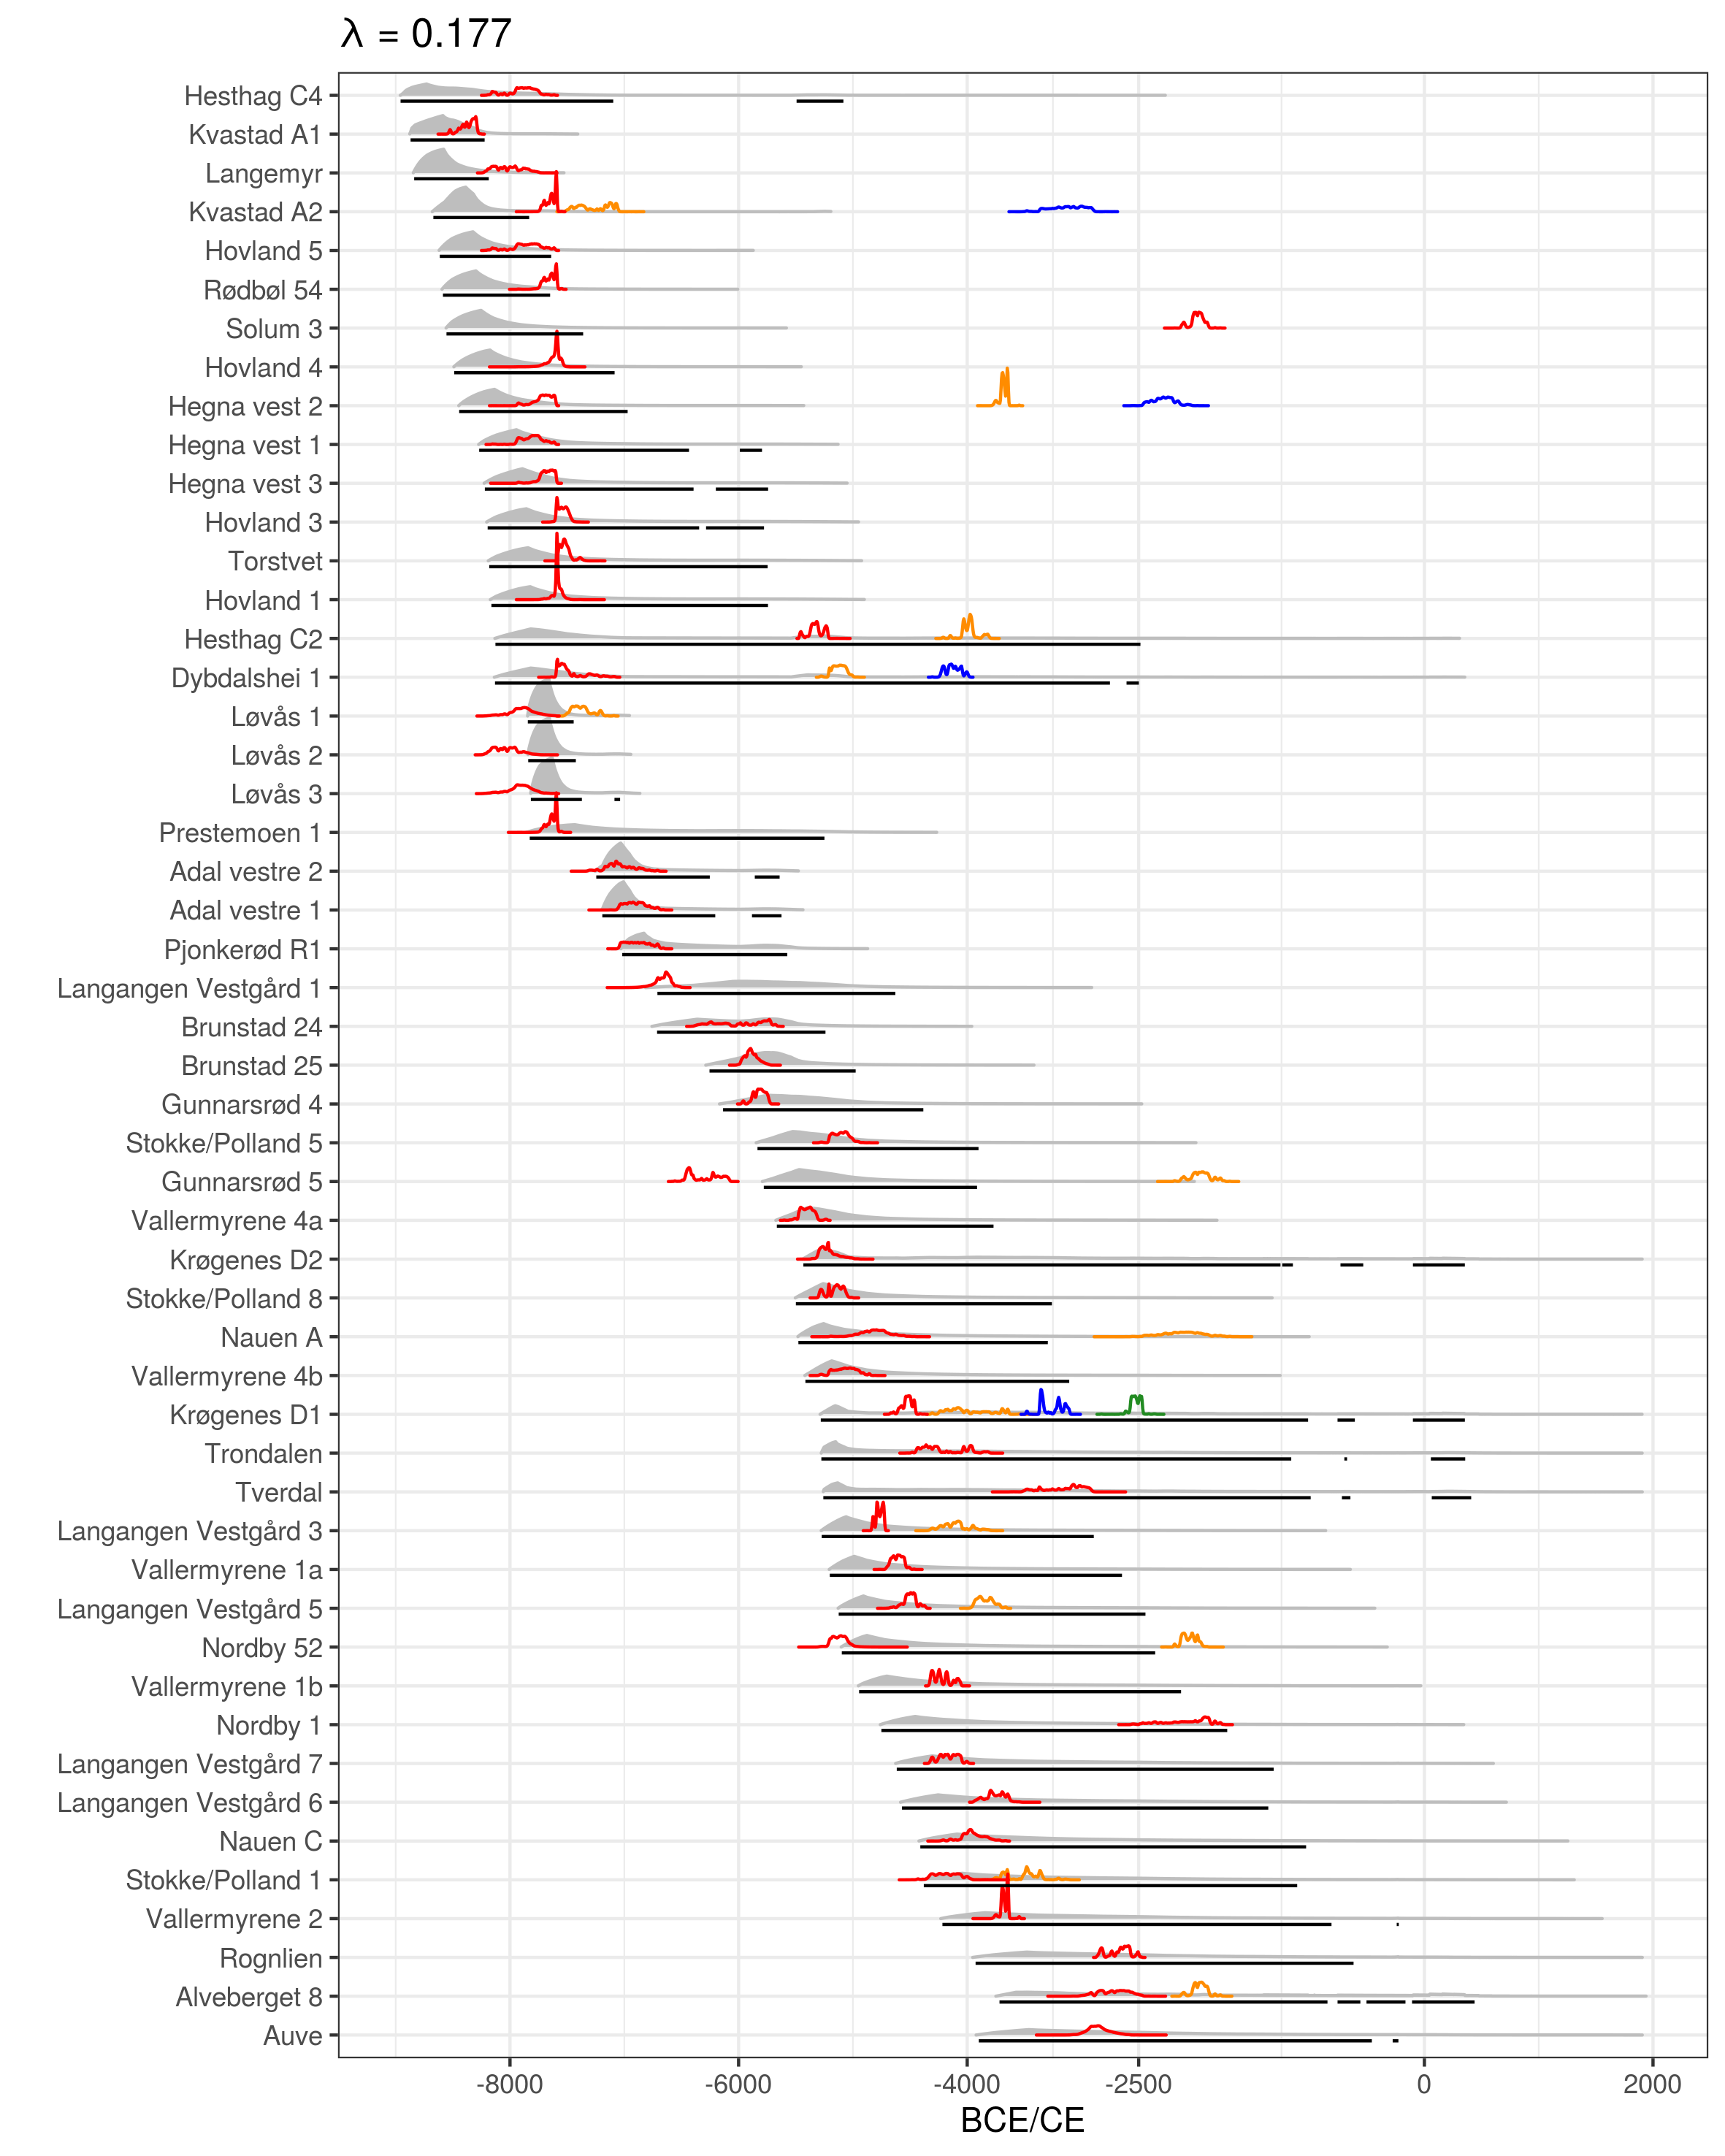
\includegraphics[width=525px]{/home/isak/phd/assessing.sealevel.dating/analysis/figures/shoredate} 

}

\caption{The result of backwards shoreline dating the sites with radiocarbon dates corresponding to the artefact inventory using the method proposed here. The shoreline dates are plotted in grey and underlined with the 95\% HDR in black. These are plotted against the modelled radiocarbon dates, which are given colour from oldest to youngest occupation phase for each site, defined by non-overlapping dates at 99.7\% probability.}\label{fig:shoredate}
\end{figure}

\begin{figure}

{\centering 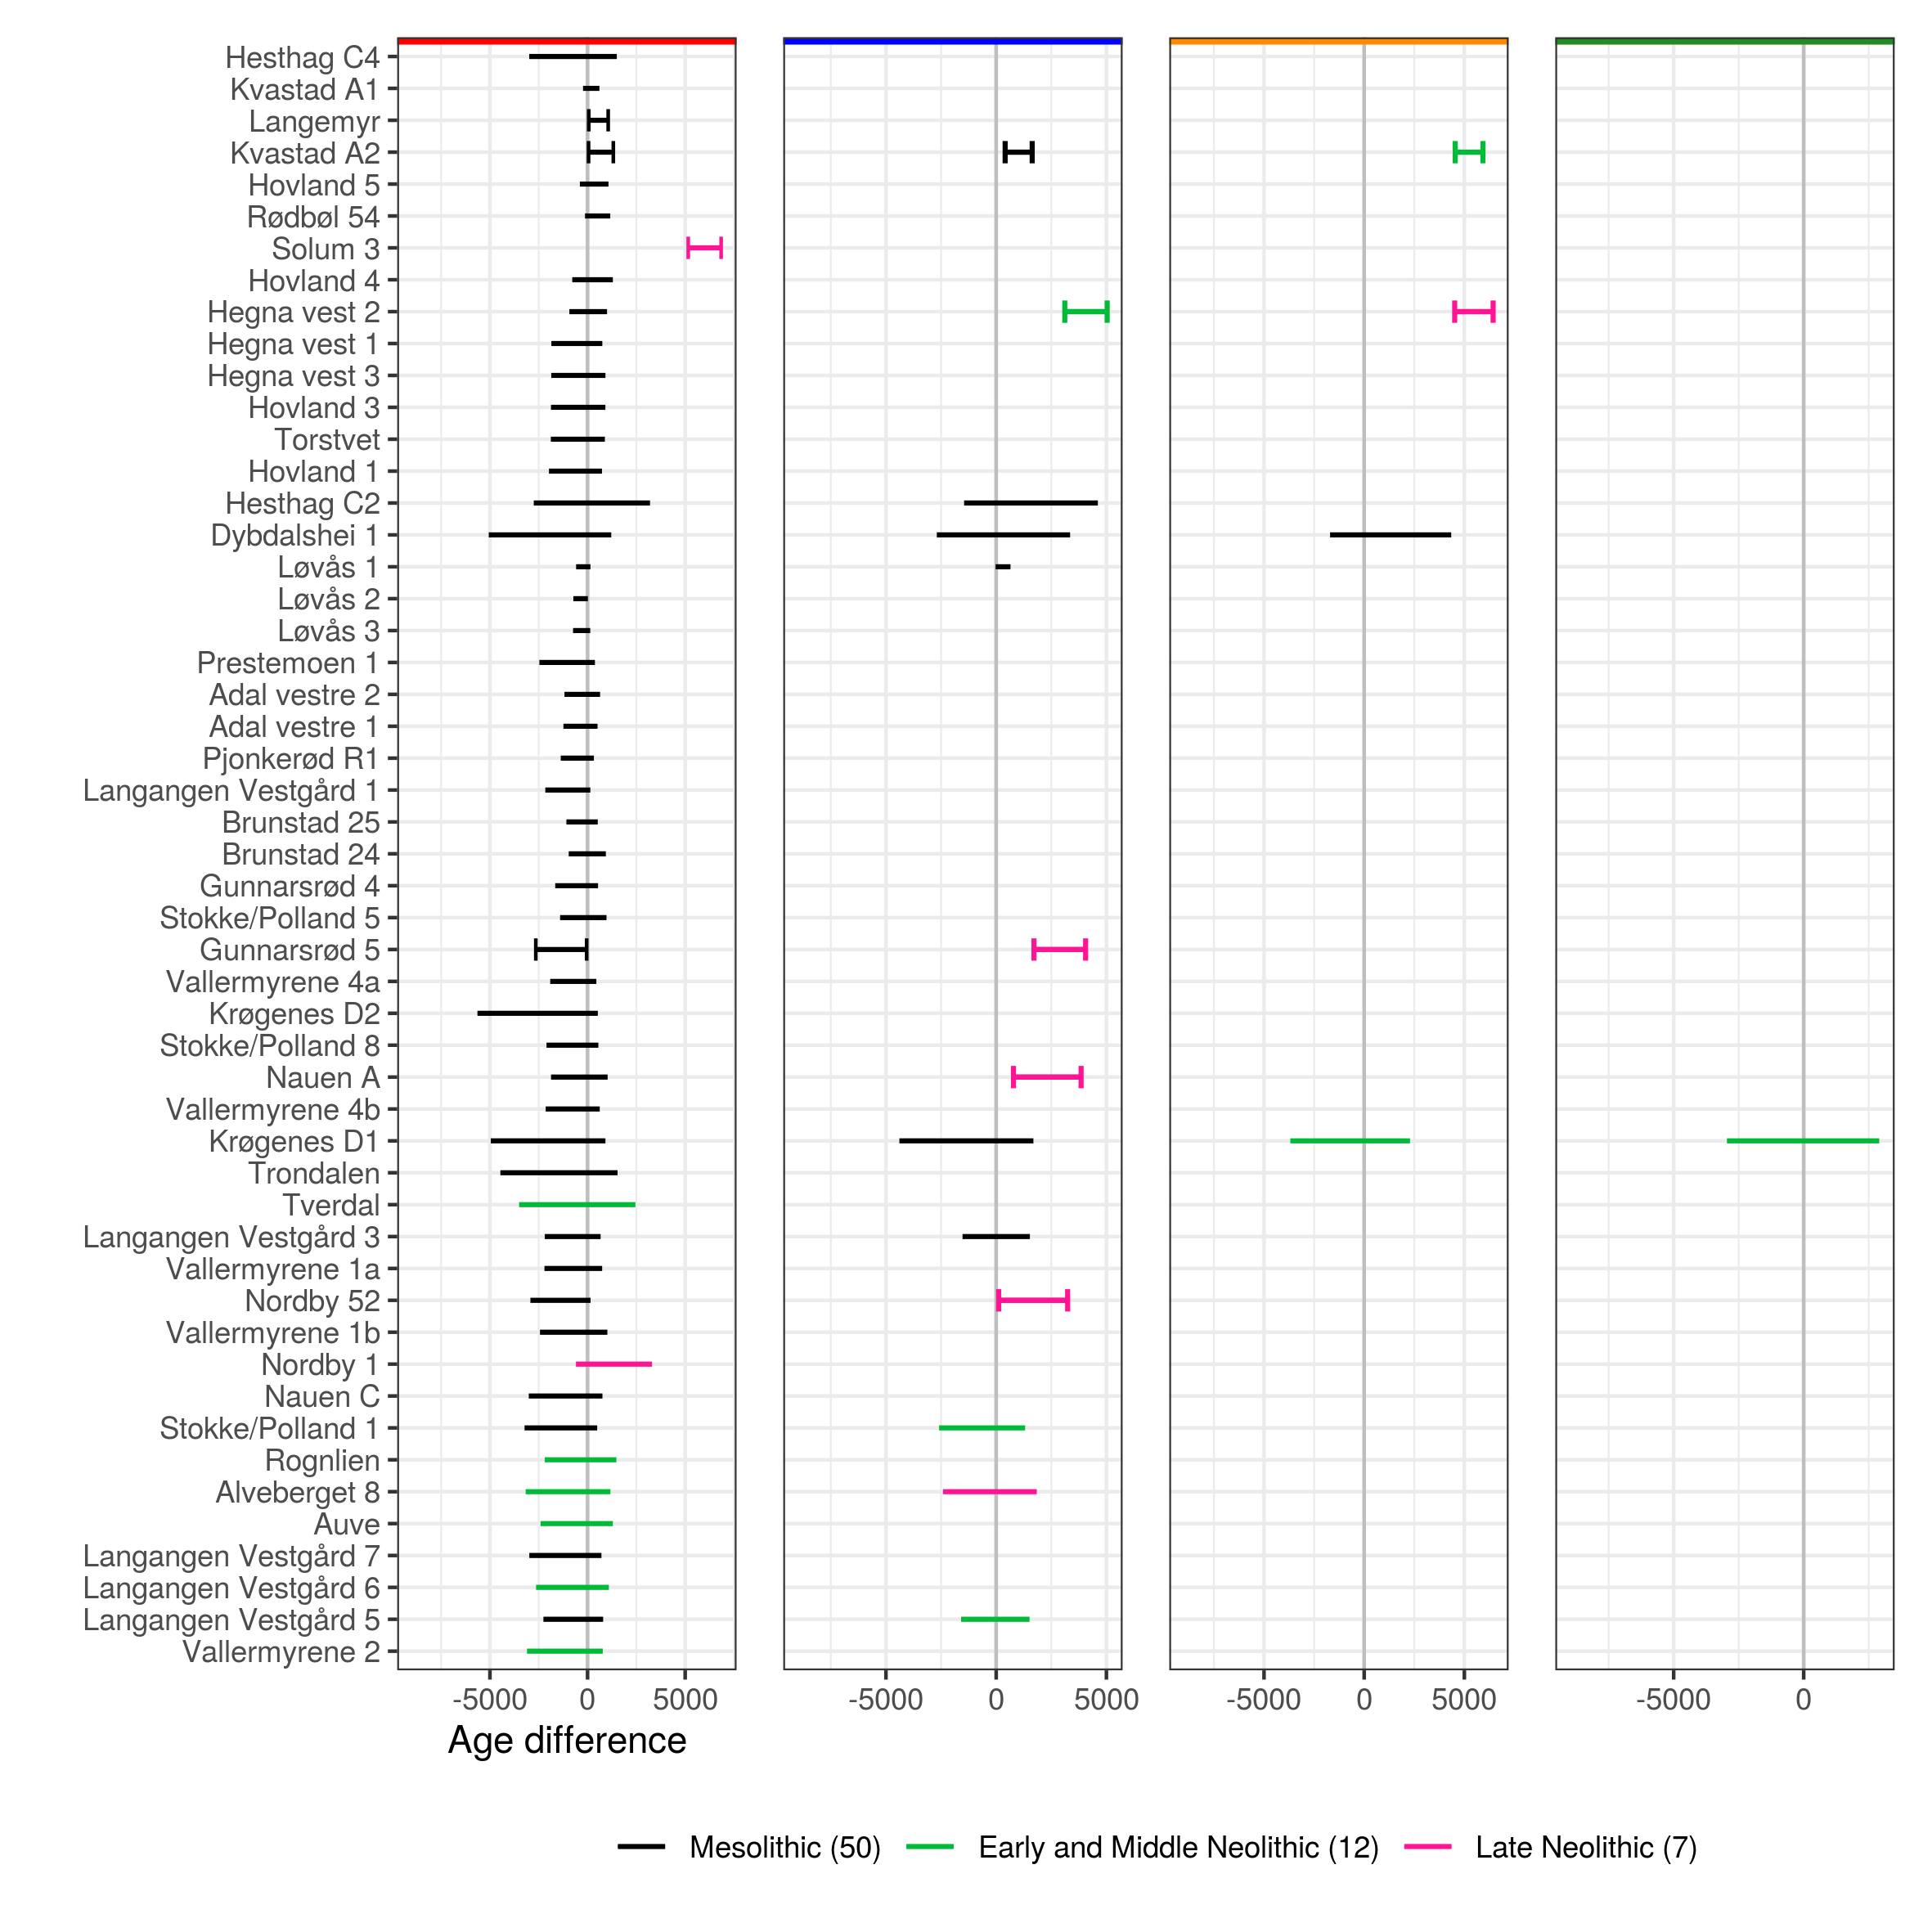
\includegraphics[width=525px]{/home/isak/phd/assessing.sealevel.dating/analysis/figures/shoredate2} 

}

\caption{Evaluation of the agreement between the shoreline dates and radiocarbon dates given in Figure 8. When the range of the 95\% HDR for age difference crosses zero, the shoreline and radiocarbon dates are considered synchronous. Line segments with vertical bars indicate that this does not cross zero and that the dates are not in agreement.  The division and colour coding at the top of the plots reflect the divison of site phases given in Figure 8.}\label{fig:shoredatediff}
\end{figure}

\hypertarget{re-dating-previously-shoreline-dated-sites}{%
\section{Re-dating previously shoreline dated sites}\label{re-dating-previously-shoreline-dated-sites}}

To further explore the implementation for shoreline dating presented above, excavated and shoreline dated Stone Age sites within the study area where \textsuperscript{14}C-dates are not available or these are not believed to date the main occupation of the sites have been subjected to the outlined approach (Figure \ref{fig:redate}). The resulting dates are compared to those originally proposed in the excavation reports for the sites (the numerical results are available in the supplementary material). To avoid issues with recent disturbances on the DTM, the sites have been dated based on the mean of the altitudes provided in the report for each site.

The comparison with previously reported dates is an illustrative, but unfair exercise for a few reasons. First of all the dates provided in the reports are typically stated to be a very rough estimate, and are sometimes given as a point estimate with an undefined, but implied or explicit uncertainty range. Secondly, seeing as these reports are from various dates in time, many are based on now outdated data on RSL-change. Finally, they are sometimes only meant to indicate a lower bound for when the sites could have been in use. Overall, the results suggest that shoreline dating has generally been applied with a fairly reasonable degree of success, seeing as these dates have typically been interpreted and informed research in an approximate manner (although see e.g. Roalkvam 2022). That being said, the results do also indicate that shoreline dating has at times been applied with an exaggerated degree of precision. While the implications of a more stable RSL-change for the duration of use and re-use of site locations are well known, this also appears to be somewhat under-appreciated for the purposes of shoreline dating. The results also highlight the spatial and temporal contingency of the method, illustrated by the variation in the range of the 95\% HDRs for the dates. In some cases the method provides a very precise date range and in others it offers little more than a \emph{terminus post quem}. This is dependent on the steepness of the displacement curves, leading to the general pattern of older sites situated towards the north-east getting more precise dates (cf.~Figure \ref{fig:map-iso}B). Further, as some of the date ranges extend well beyond major chronological divisions, even into the Iron Age, they could be severely and securely constrained with only cursory reference to typology. While this would be trivial in some cases, the nature and uncertainty inherent to the method still means that this is arguably a required exercise that should be explicitly performed. This also points to the possibility of drawing on other temporal data, for example within a Bayesian framework, to further improve the precision of the dates that can be achieved with shoreline dating.

\begin{figure}

{\centering 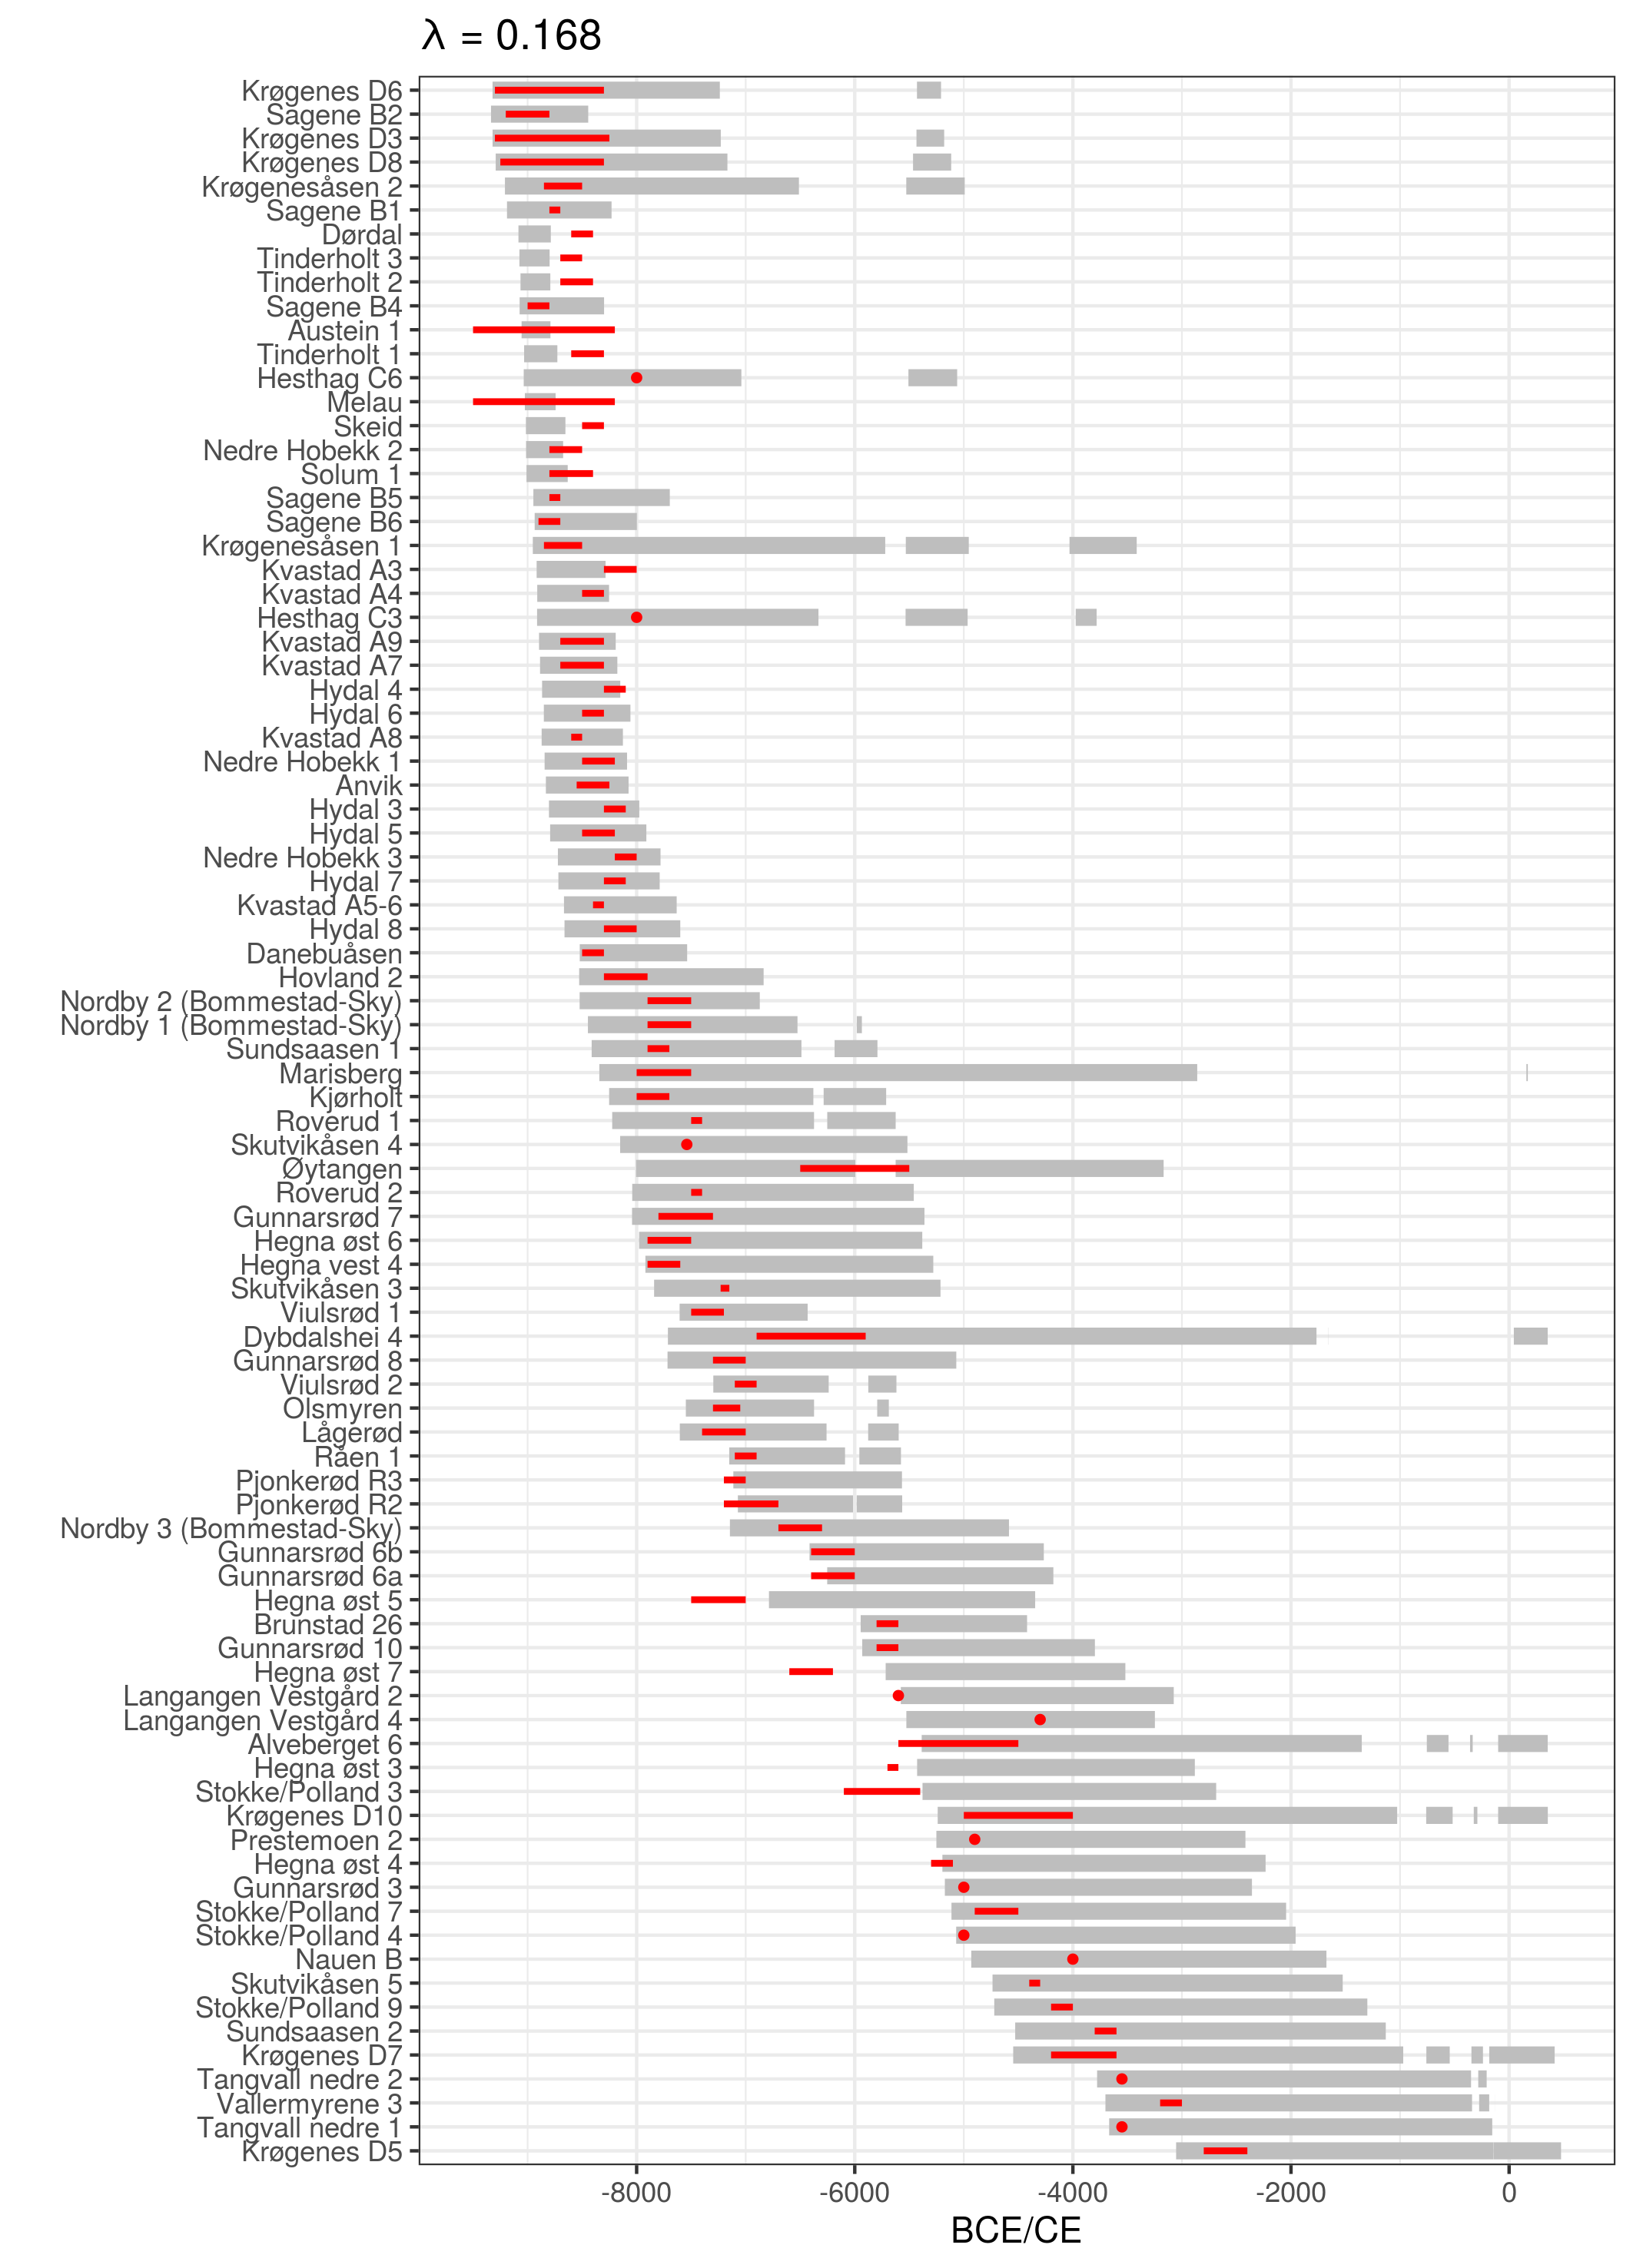
\includegraphics[width=525px]{/home/isak/phd/assessing.sealevel.dating/analysis/figures/redate} 

}

\caption{Re-dating excavated and previously shoreline dated sites in the study area without radiocarbon dates or with radiocarbon dates that do not correspond to the artefact inventories. The 95\% HDRs in grey are compared to the dates originally proposed by the excavation reports in red.}\label{fig:redate}
\end{figure}

Not least following from the fact that relatively few Preboreal \textsuperscript{14}C-dates associated with anthropogenic activity have been achieved in Norway (Åstveit 2018; Damlien and Solheim 2018; Kleppe 2018), the shoreline dating of the earliest sites is essential for understanding the pioneer settlement and the initial colonisation of the Scandinavian peninsula (e.g. Bang-Andersen 2012; Berg-Hansen 2018; Breivik 2014; Fuglestvedt 2012; Glørstad 2016). The shoreline dated Preboreal sites from the Brunlanes-project are among the earliest known sites in Norway (Jaksland 2012a, 2012b; Jaksland and Persson 2014). These have a distinct Early Mesolithic artefact inventory and are situated in a steep area of the landscape where it would be difficult to envision use of the sites after the sea retreated any significant distance from their location. In the original publication of the sites, Jaksland (2014) provides a thorough discussion of shoreline dating in general, and as used for the dating of the Brunlanes sites specifically. A comparison of his results and the ones achieved using the above-outlined approach are given in Figure \ref{fig:brunlanes}A. The sites have been dated using what Jaksland (2014) gives as the lowest elevation of finds at each site, and by employing a exponential decay ratio of 0.13, to allow for more deviance in the distance between site and shoreline. This corresponds to the decay ratio for sites older than 7000 BCE in Figure \ref{fig:results2}.

The small discrepancies between the achieved results mainly follow from the fact that a slightly updated version of the local displacement curve is applied here (cf. Sørensen et al. in prep). Jaksland's dates are given a flat 200 and 50 year uncertainty range starting from what he gives as the earliest possible date. The 200 year uncertainty range is given if the sites were to be considered in isolation, while the argument for the uncertainty range of only 50 years is based on the location of the sites relative to each other. Since they are located in such a constrained and steep area of the landscape, the difference in elevation between the sites is argued to establish their relative date and thus constrain the uncertainty ranges so that they don't overlap. This information is not integrated in the approach outlined here, but could justify further reducing the uncertainty ranges. Although their accuracy is of course ultimately dependent on the veracity of the geological reconstruction, the high rate of RSL-change in this period does result in very precise dates. Above it was suggested that additional temporal data could be combined with the method to improve its accuracy and precision. This example, on the other hand, highlights the fact that the spatial nature of the method means that a consideration of the surrounding terrain and other sites can also help in increasing the precision of the method if this can be used to exclude certain sea-levels as unlikely for when a site was in use. One approach could also be to assess the spatial implication of a proposed shoreline date by simulating the adjusted sea-levels, as is done for Pauler 1 in Figure \ref{fig:brunlanes}B, followed for example by a visual evaluation of the topography or by evaluating the distance and steepness of the slope to the shoreline. If this is developed further, it could conceivably be possible to exclude certain elevations as unlikely for the position of the shoreline when the site was in use. Such approaches would make less of an impact in this setting, where the 95\% HDR is already quite constrained, but could considerably improve the precision of the method in cases where RSL-change has been less severe (cf.~Figure \ref{fig:redate}).

\begin{figure}

{\centering 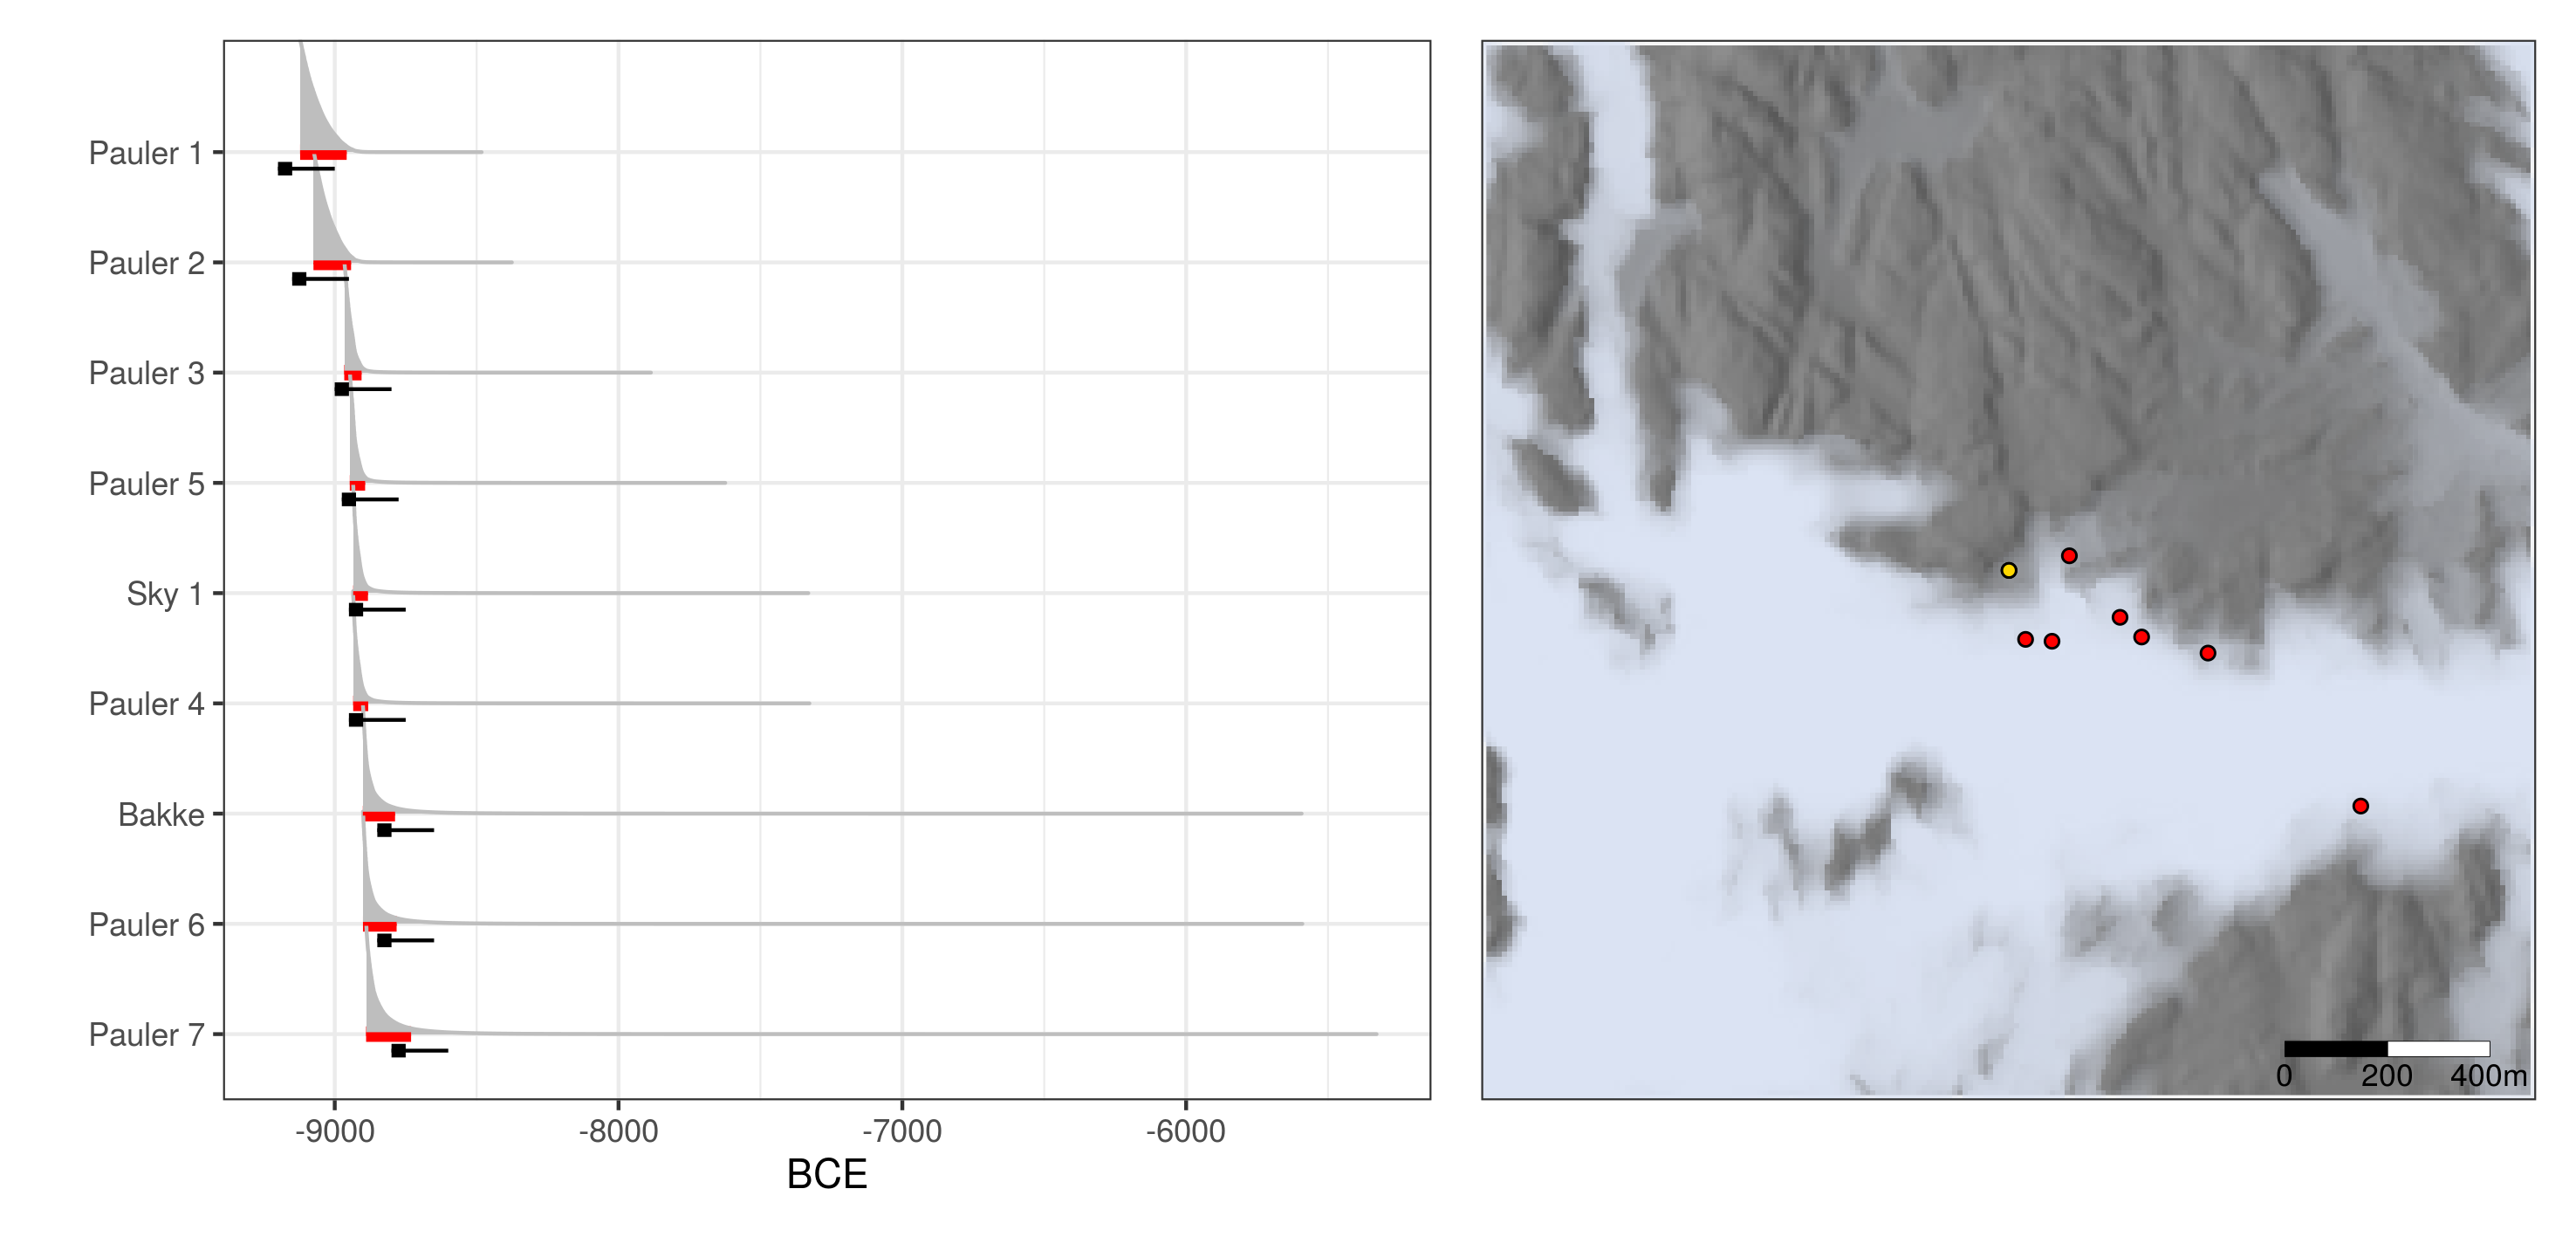
\includegraphics[width=525px]{/home/isak/phd/assessing.sealevel.dating/analysis/figures/brunlanes} 

}

\caption{Shoreline dating of the Brunlanes sites using site altitudes provided by Jaksland (2014:tab.4). A) The result of applying the approach to shoreline dating outlined above. The shoreline date in grey is underlined with the 95\% HDR in black. Dates provided by Jaksland (2014) are plotted in red. The box indicates a 50 year uncertainty range which in combination with the red line extends 200 years. B) Map showing the centroids of the Pauler sites and Sky 1. The sea-level has been simulated using the probability density associated with the shoreline date for Pauler 1 (see also map in Jaksland 2014:fig.12a). Pauler 1 is the red point.}\label{fig:brunlanes}
\end{figure}

\hypertarget{concluding-remarks}{%
\section{Concluding remarks}\label{concluding-remarks}}

The most immediate contribution of this paper is what must be considered a confirmation of previous research into the relation between coastal Norwegian Stone Age sites and the prehistoric shoreline. This is indicated by the close relationship between sites and the shoreline up until the transition to the Neolithic at c.~4000 BCE, after which a couple of sites become situated some distance from the sea, followed by a more decisive break at the transition to the Late Neolithic at c.~2500 BCE. This development is in clear agreement with the literature. Furthermore, based on the quantitative nature of these findings, an initial formulation of a refined method for the shoreline dating of pre-Late Neolithic Stone Age sites has been proposed. Apart from taking the distance between sites and the isobases of the displacement curves into consideration when dating the sites, this involves implementing Eq. \eqref{eq:shoredate} to account for the distance between the sites and the shoreline. When no other information is available, it can at present be recommended to use the empirically derived exponential decay ratio of 0.173 (Figure \ref{fig:redate}A) to characterise this relationship. Furthermore, while this remains to be formalised and explored further, it was also showed how the accuracy of the method can be improved by including more information, both with reference to the topographic location of the sites and other temporal data. As the precision of the method is both geographically and temporally contingent due to the trajectory of RSL-change, where older sites situated towards the north-east in the study area will get a more precise date than younger sites located towards the south-west, the impact of such additional information will also vary.

Future investigations and radiocarbon dates from Stone Age sites in the region can not only be used to further evaluate and adjust the findings reported here, but a larger sample size could also lay the foundations for refining the method by identifying subsets of sites for which the application of the method could be adjusted. Given it's behavioural nature, it would for example seem likely that dimensions such as the nature and purpose of visits to the sites will have implications for how close to the shoreline they were located. Furthermore, other dimensions related to the topographic location of the sites could be similarly explored. This for example pertains to the exposure of sites to wave action, which is likely to have been of concern (Roalkvam 2020), and which presumably has implications for how close to the shoreline people settled (Blankholm 2020; Helskog 1978). This is also related to the fact that while the mean sea-level is used for dating the sites, a consideration of the tidal range could possibly also have implications for the site location relative to the shoreline, depending on the topography (Helskog 1978). The potential of dimensions such as these was also hinted at here with the estimation and cursory treatment of the horizontal and topographic distance to the shoreline. If patterns related to such locational patterns can be discerned and unpicked, this will not least be useful for improving the shoreline dating of sites which have only been surveyed and where little information beyond their location is available.

Some limitations and sources of likely variation and uncertainty that have not been considered should also be mentioned. First of all the sample size is quite strained and the future addition more sites might alter the picture considerably. Secondly, the DTM has only been corrected for major modern disturbances. This means that other forms of erosion, although likely not that prevalent, has not been taken into account. Thirdly, the DTM has a vertical error which could also benefit from being integrated in the analysis (cf. Lewis 2021). Fourthly, the displacement curves were here interpolated to all site locations without accounting for increased uncertainty as one moves further away from the isobases of the displacement curves. This is also related to the fact that the RSL data can be handled in different ways than with the isobase method that has been used for the compilation of the employed displacement curves (cf. Creel et al. 2022). Fifthly, neither the question of how site limits are defined nor the elevation range over which these extend was given much consideration (cf. Mjærum 2022). Finally, the radiocarbon dates and division of settlement phases at each site was here simply done by treating radiocarbon dates not overlapping at 99.7\% as representing unrelated occupation events. This could also be handled differently (e.g. Bronk Ramsey 2009, 2015). While each of these factors will have variable impact on the final results, they clearly represent dimensions which would all benefit from further consideration.

Finally, this analysis employed a simulation approach to integrate multiple sources of spatio-temporal uncertainty. Here this was simply used to inform the question of the distance between sites and the shoreline. However, this method and general framework can be extended to a wide range of use-cases where one needs to visualise, and quantitatively or qualitatively evaluate the relationship between archaeological phenomena, the prehistoric shoreline, and the uncertainty inherent in this reconstruction.

\newpage

\hypertarget{references}{%
\section{References}\label{references}}

\hypertarget{refs}{}
\begin{CSLReferences}{0}{0}
\leavevmode\vadjust pre{\hypertarget{ref-akerlund1996}{}}%
\CSLBlock{Åkerlund, Agneta}
\CSLLeftMargin{ 1996}
\CSLRightInline{\emph{{Human responses to shore displacement: Living by the sea in Eastern Middle Sweden during the Stone Age}}. Riksantikvarieämbetet, Stockholm.}

\leavevmode\vadjust pre{\hypertarget{ref-akerlund1995}{}}%
\CSLBlock{Åkerlund, Agneta, Jan Risberg, Urve Miller, and Per Gustafsson}
\CSLLeftMargin{ 1995}
\CSLRightInline{{On the applicability of the \(^{14}\)C method to interdisciplinary studies on shore displacement and settlement location}. \emph{PACT} 49:53--84.}

\leavevmode\vadjust pre{\hypertarget{ref-amundsen2006}{}}%
\CSLBlock{Amundsen, Øystein, Stig Knutsen, Axel Mjærum, and Gaute Reitan}
\CSLLeftMargin{ 2006}
\CSLRightInline{{Nøkleby i Ski -- en tidligneolittisk jordbruksboplass?} \emph{Primitive tider} 9:85--96.}

\leavevmode\vadjust pre{\hypertarget{ref-uxe5stveit2018}{}}%
\CSLBlock{Åstveit, Leif Inge}
\CSLLeftMargin{ 2018}
\CSLRightInline{{The Early Mesolithic of Western Norway}. In \emph{{Early Economy and Settlement in Northern Europe. Pioneering, Resource Use, Coping with Change}}, edited by Hans Peter Blankholm, pp. 231--274. Equinox, Sheffield.}

\leavevmode\vadjust pre{\hypertarget{ref-bakka1971}{}}%
\CSLBlock{Bakka, Egil, and Peter Emil Kaland}
\CSLLeftMargin{ 1971}
\CSLRightInline{Early farming in Hordaland, western Norway. Problems and approaches in archaeology and pollen analysis. \emph{Norwegian Archaeological Review} 4:1--17. DOI:\href{https://doi.org/10.1080/00293652.1971.9965136}{10.1080/00293652.1971.9965136}.}

\leavevmode\vadjust pre{\hypertarget{ref-bang-andersen2012}{}}%
\CSLBlock{Bang-Andersen, Sveinung}
\CSLLeftMargin{ 2012}
\CSLRightInline{Colonizing Contrasting Landscapes. The Pioneer Coast Settlement and Inland Utilization in Southern Norway 10,000-9500 Years Before Present. \emph{Oxford Journal of Archaeology} 31:103--120. DOI:\href{https://doi.org/10.1111/j.1468-0092.2012.00381.x}{10.1111/j.1468-0092.2012.00381.x}.}

\leavevmode\vadjust pre{\hypertarget{ref-berg-hansen2009}{}}%
\CSLBlock{Berg-Hansen, Inger Marie}
\CSLLeftMargin{ 2009}
\CSLRightInline{\emph{{Steinalderregistrering. Metodologi og forskningshistorie i Norge 1900-2000 med en feltstudie fra Lista i Vest-Agder}}. Museum of Cultural History, University of Oslo, Oslo.}

\leavevmode\vadjust pre{\hypertarget{ref-berg-hansen2018}{}}%
\CSLLeftMargin{ 2018 }
\CSLRightInline{{Continuity and Change in Late- and Post-glacial Social Networks: Knowledge Transmission and Blade Production Methods in Ahrensburgian and Early Mesolithic North West Europe}. In \emph{{The Early Settlement of Northern Europe. Transmission of Knowledge and Culture}}, edited by Kjel Knutsson, Helena Knutsson, Jan Apel, and Håkon Glørstad, pp. 63--98. Equinox, Sheffield.}

\leavevmode\vadjust pre{\hypertarget{ref-bergsvik2009}{}}%
\CSLBlock{Bergsvik, Knut Andreas}
\CSLLeftMargin{ 2009}
\CSLRightInline{{Caught in the middle: functional and ideological aspects of Mesolithic shores in Norway}. In \emph{{Mesolithic Horizons: Papers presented at the Seventh International Conference on the Mesolithic in Europe, Belfast 2005}}, edited by Sinéad B. McCartan, Rick Schulting, Graeme Warren, and Peter Woodman, pp. 602--609. Oxbow Books, Oxford.}

\leavevmode\vadjust pre{\hypertarget{ref-bevan2013a}{}}%
\CSLBlock{Bevan, Andrew, Enrico R. Crema, Xiuzhen Li, and Alessio Palmisano}
\CSLLeftMargin{ 2013}
\CSLRightInline{{Intensities, Interactions, and Uncertainties: Some New Approaches to Archaeological Distributions}. In \emph{{Computational Approaches to Archaeological Spaces}}, edited by Andrew Bevan and Mark Lake, pp. 27--52. Left Coast Press, Walnut Creek.}

\leavevmode\vadjust pre{\hypertarget{ref-bivand2021}{}}%
\CSLBlock{Bivand, Roger}
\CSLLeftMargin{ 2021}
\CSLRightInline{\emph{{rgrass7: Interface Between GRASS 7 Geographical Information System and R. R package version 0.2-6.}}}

\leavevmode\vadjust pre{\hypertarget{ref-bjerck1990}{}}%
\CSLBlock{Bjerck, Hein Bjartmann}
\CSLLeftMargin{ 1990}
\CSLRightInline{{Mesolithic site types and settlement patterns at Vega, Northern Norway}. \emph{Acta Archaeologica} 60:1--32.}

\leavevmode\vadjust pre{\hypertarget{ref-bjerck2005}{}}%
\CSLLeftMargin{ 2005 }
\CSLRightInline{Strandlinjedatering. In \emph{Norsk arkeologisk leksikon}, edited by Einar Østmo and Lotte Hedeager, pp. 363--364. Pax, Oslo.}

\leavevmode\vadjust pre{\hypertarget{ref-bjerck2008}{}}%
\CSLLeftMargin{ 2008a }
\CSLRightInline{{Norwegian Mesolithic Trends: A Review}. In \emph{{Mesolithic Europe}}, edited by Geoff Bailey and Penny Spikins, pp. 60--106. Cambridge University Press, Cambridge.}

\leavevmode\vadjust pre{\hypertarget{ref-bjerck2008a}{}}%
\CSLLeftMargin{ 2008b }
\CSLRightInline{Innledende betraktninger. In \emph{{NTNU Vitenskapsmuseets arkeologiske undersøkelser Ormen Lange Nyhamna}}, edited by Hein Bjartmann Bjerck, Leif Inge Åstveit, Trond Meling, Jostein Gundersen, Guro Jørgensen, and Staale Normann, pp. 548--551. Tapir Akademisk Forlag, Trondheim.}

\leavevmode\vadjust pre{\hypertarget{ref-blankholm2020}{}}%
\CSLBlock{Blankholm, Hans Peter}
\CSLLeftMargin{ 2020}
\CSLRightInline{{In the wake of the wake. An investigation of the impact of the Storegga tsunami on the human settlement of inner Varangerfjord, northern Norway}. \emph{Quaternary International} 549:65--73. DOI:\url{https://doi.org/10.1016/j.quaint.2018.05.050}.}

\leavevmode\vadjust pre{\hypertarget{ref-breivik2014}{}}%
\CSLBlock{Breivik, Heidi Mjelva}
\CSLLeftMargin{ 2014}
\CSLRightInline{Palaeo-oceanographic development and human adaptive strategies in the Pleistocene--Holocene transition: A study from the Norwegian coast. \emph{The Holocene} 24:1478--1490. DOI:\href{https://doi.org/10.1177/0959683614544061}{10.1177/0959683614544061}.}

\leavevmode\vadjust pre{\hypertarget{ref-breivik2018}{}}%
\CSLBlock{Breivik, Heidi Mjelva, Guro Fossum, and Steinar Solheim}
\CSLLeftMargin{ 2018}
\CSLRightInline{Exploring human responses to climatic fluctuations and environmental diversity: Two stories from Mesolithic Norway. \emph{Quaternary International} 465. Impacts of gradual and abrupt environmental changes on Late glacial to Middle Holocene cultural changes in Europe:258--275. DOI:\href{https://doi.org/10.1016/j.quaint.2016.12.019}{10.1016/j.quaint.2016.12.019}.}

\leavevmode\vadjust pre{\hypertarget{ref-breivik2018a}{}}%
\CSLBlock{Breivik, Heidi, and Hein Bjartmann Bjerck}
\CSLLeftMargin{ 2018}
\CSLRightInline{{Early Mesolithic Central Norway: A Review of Research History, Settlements, and Tool Tradition}. In \emph{{Early Economy and Settlement in Northern Europe. Pioneering, Resource Use, Coping with Change}}, edited by Hans Peter Blankholm, pp. 169--206. Equinox, Sheffield.}

\leavevmode\vadjust pre{\hypertarget{ref-brogger1905}{}}%
\CSLBlock{Brøgger, Waldemar Christofer}
\CSLLeftMargin{ 1905}
\CSLRightInline{\emph{{Strandliniens Beliggenhed under Stenalderen i Det Sydøstlige Norge}}. Norges geologiske undersøkelse, Kristiania.}

\leavevmode\vadjust pre{\hypertarget{ref-bronkramsey2009}{}}%
\CSLBlock{Bronk Ramsey, Christopher}
\CSLLeftMargin{ 2009}
\CSLRightInline{Bayesian Analysis of Radiocarbon Dates. \emph{Radiocarbon} 51(1):337--360. DOI:\href{https://doi.org/10.1017/S0033822200033865}{10.1017/S0033822200033865}.}

\leavevmode\vadjust pre{\hypertarget{ref-bronkramsey2015}{}}%
\CSLLeftMargin{ 2015 }
\CSLRightInline{{Bayesian Approaches to the Building of Archaeological Chronologies}. In \emph{{Mathematics and Archaeology}}, edited by Juan A. Barcelo and Igor Bogdanovic, pp. 272--292. CRC Press, Boca Raton.}

\leavevmode\vadjust pre{\hypertarget{ref-conolly2020}{}}%
\CSLBlock{Conolly, James}
\CSLLeftMargin{ 2020}
\CSLRightInline{Spatial interpolation. In \emph{{Archaeological Spatial Analysis: A Methodological Guide}}, edited by Mark Gillings, Piraye Hacıgüzeller, and Gary Lock, pp. 118--134. Routledge, London \& New York.}

\leavevmode\vadjust pre{\hypertarget{ref-conolly2006}{}}%
\CSLBlock{Conolly, James, and Mark Lake}
\CSLLeftMargin{ 2006}
\CSLRightInline{\emph{{Geographical Information Systems in Archaeology}}. Cambridge University Press, Cambridge.}

\leavevmode\vadjust pre{\hypertarget{ref-creel2022}{}}%
\CSLBlock{Creel, Roger C., Jacqueline Austermann, Nicole S. Khan, William J. D'Andrea, Nicholas Balascio, Blake Dyer, Erica Ashe, and William Menke}
\CSLLeftMargin{ 2022}
\CSLRightInline{Postglacial relative sea level change in Norway. \emph{Quaternary Science Reviews} 282:107422. DOI:\href{https://doi.org/10.1016/j.quascirev.2022.107422}{10.1016/j.quascirev.2022.107422}.}

\leavevmode\vadjust pre{\hypertarget{ref-crema2012}{}}%
\CSLBlock{Crema, Enrico R.}
\CSLLeftMargin{ 2012}
\CSLRightInline{Modelling Temporal Uncertainty in Archaeological Analysis. \emph{Journal of Archaeological Method and Theory} 19(3):440--461. DOI:\href{https://doi.org/10.1007/s10816-011-9122-3}{10.1007/s10816-011-9122-3}.}

\leavevmode\vadjust pre{\hypertarget{ref-crema2015}{}}%
\CSLLeftMargin{ 2015 }
\CSLRightInline{{Time and Probabilistic Reasoning in Settlement Analysis}. In \emph{{Mathematics and Archaeology}}, edited by Juan A. Barcelo and Igor Bogdanovic, pp. 314--334. CRC Press, Boca Raton.}

\leavevmode\vadjust pre{\hypertarget{ref-crema2010}{}}%
\CSLBlock{Crema, Enrico R., Andrew Bevan, and Mark W. Lake}
\CSLLeftMargin{ 2010}
\CSLRightInline{A probabilistic framework for assessing spatio-temporal point patterns in the archaeological record. \emph{Journal of Archaeological Science} 37(5):1118--1130. DOI:\href{https://doi.org/10.1016/j.jas.2009.12.012}{10.1016/j.jas.2009.12.012}.}

\leavevmode\vadjust pre{\hypertarget{ref-damlien2018b}{}}%
\CSLBlock{Damlien, Hege, and Steinar Solheim}
\CSLLeftMargin{ 2018}
\CSLRightInline{{The Pioneer Settlement of Eastern Norway}. In \emph{{Early Economy and Settlement in Northern Europe. Pioneering, Resource Use, Coping with Change}}, edited by Hans Peter Blankholm, pp. 335--367. Equinox, Sheffield.}

\leavevmode\vadjust pre{\hypertarget{ref-degeer1896}{}}%
\CSLBlock{De Geer, Gerard}
\CSLLeftMargin{ 1896}
\CSLRightInline{\emph{{Om Skandinaviens geografiska utveckling efter Istiden}}. P. A. Norstedt \& Söner, Stockholm.}

\leavevmode\vadjust pre{\hypertarget{ref-eskeland2017}{}}%
\CSLBlock{Eskeland, Knut Fossdal}
\CSLLeftMargin{ 2017}
\CSLRightInline{\emph{{Rapport, arkeologisk registrering. E18 Langangen Rugtvedt, 16/06999, Porsgrunn og Bamble kommune}}. Skien.}

\leavevmode\vadjust pre{\hypertarget{ref-fossum2020}{}}%
\CSLBlock{Fossum, Guro}
\CSLLeftMargin{ 2020}
\CSLRightInline{{Specialists facing climate change. The 8200 cal BP event and its impact on the coastal settlement in the inner Oslo fjord, southeast Norway}. In \emph{{Coastal Landscapes of the Mesolithic: Human Engagement with the Coast from the Atlantic to the Baltic Sea}}, edited by Almut Schülke, pp. 179--201. Routledge, London \& New York.}

\leavevmode\vadjust pre{\hypertarget{ref-fuglestvedt2012}{}}%
\CSLBlock{Fuglestvedt, Ingrid}
\CSLLeftMargin{ 2012}
\CSLRightInline{{The Pioneer Condition on the Scandinavian Peninsula: the Last Frontier of a {`}Palaeolithic Way{'} in Europe}. \emph{Norwegian Archaeological Review} 45(1):1--29. DOI:\href{https://doi.org/10.1080/00293652.2012.669998}{10.1080/00293652.2012.669998}.}

\leavevmode\vadjust pre{\hypertarget{ref-gjerpe2008b}{}}%
\CSLBlock{Gjerpe, Lars Erik, and Grethe Bjørkan Bukkemoen}
\CSLLeftMargin{ 2008}
\CSLRightInline{{Nordby 1 -- Toskipede hus fra neolitikum-bronsealder og boplasspor fra jernalder}. In \emph{{E18-prosjektet Vestfold. Bind 3. Hus, boplass- og dyrkningsspor}}, edited by Lars Erik Gjerpe, pp. 7--38. University of Oslo, Museum of Cultural History, Oslo.}

\leavevmode\vadjust pre{\hypertarget{ref-glorstad2010}{}}%
\CSLBlock{Glørstad, Håkon}
\CSLLeftMargin{ 2010}
\CSLRightInline{\emph{{The Structure and History of the Late Mesolithic Societies in the Oslo Fjord Area 6300-3800 BC}}. Bricoleur Press, Lindome.}

\leavevmode\vadjust pre{\hypertarget{ref-glorstad2012}{}}%
\CSLLeftMargin{ 2012 }
\CSLRightInline{{Historical ideal types and the transition to the Late Neolithic in South Norway}. In \emph{{Becoming European. The transformation of third millenium Northern and Western Europe}}, edited by Christopher Prescott and Håkon Glørstad, pp. 82--99. Oxbow Books, Oxford \& Oakville.}

\leavevmode\vadjust pre{\hypertarget{ref-glorstad2016}{}}%
\CSLLeftMargin{ 2016 }
\CSLRightInline{Deglaciation, sea-level change and the Holocene colonization of Norway. \emph{Geological Society, London, Special Publications} 411:9--25. DOI:\href{https://doi.org/10.1144/SP411.7}{10.1144/SP411.7}.}

\leavevmode\vadjust pre{\hypertarget{ref-glorstad2020}{}}%
\CSLBlock{Glørstad, Håkon, Jostein Gundersen, Frode Kvalø, Pål Nymoen, David Simpson, and Birgitte Skar}
\CSLLeftMargin{ 2020}
\CSLRightInline{{Submerged Stone Age from a Norwegian Perspective}. In \emph{{The Archaeology of Europe's Drowned Landscapes}}, edited by Geoff Bailey, Nena Galanidou, Hans Peeters, Hauke Jöns, and Moritz Mennenga, pp. 125-\/-140. Springer, Cham.}

\leavevmode\vadjust pre{\hypertarget{ref-grass2017}{}}%
\CSLBlock{GRASS Development Team}
\CSLLeftMargin{ 2017}
\CSLRightInline{\emph{{Geographic Resources Analysis Support System (GRASS) Software, Version 7.2}}. Open Source Geospatial Foundation.}

\leavevmode\vadjust pre{\hypertarget{ref-gundersen2013}{}}%
\CSLBlock{Gundersen, Jostein}
\CSLLeftMargin{ 2013}
\CSLRightInline{{Verken fjord eller fjell -- steinalderen i det kystnære innlandet. Gamle og nye funn fra Notodden i Telemark}. \emph{Viking} 76:35--62.}

\leavevmode\vadjust pre{\hypertarget{ref-hafsten1957}{}}%
\CSLBlock{Hafsten, Ulf}
\CSLLeftMargin{ 1957}
\CSLRightInline{{De senkvartære strandlinje-forskyvningene i Oslotrakten belyst ved pollenanalytiske undersøkelser}. \emph{Norwegian Journal of Geography} 16(1-8):74--99. DOI:\href{https://doi.org/10.1080/00291955708622137}{10.1080/00291955708622137}.}

\leavevmode\vadjust pre{\hypertarget{ref-hafsten1983}{}}%
\CSLLeftMargin{ 1983 }
\CSLRightInline{{Shore-level changes in South Norway during the last 13,000 years, traced by biostratigraphical methods and radiometric datings}. \emph{Norwegian Journal of Geography} 37(2):63--79. DOI:\href{https://doi.org/10.1080/00291958308552089}{10.1080/00291958308552089}.}

\leavevmode\vadjust pre{\hypertarget{ref-hagen1963}{}}%
\CSLBlock{Hagen, Anders}
\CSLLeftMargin{ 1963}
\CSLRightInline{{Problemkompleks Fosna. Opphav -- kontakt med kontinentale grupper -- forholdet til Komsa}. In \emph{{Boplatsproblem vid Kattegat och Skagerack}}, pp. 53--59. Göteborg och Bohusläns fornminnesförening \& Institutionen för nordisk fornkunskap, Gothenburg University, Gothenburg.}

\leavevmode\vadjust pre{\hypertarget{ref-helskog1978}{}}%
\CSLBlock{Helskog, Knut}
\CSLLeftMargin{ 1978}
\CSLRightInline{Late Holocene sea-level changes seen from prehistoric settlements. \emph{Norwegian Journal of Geography} 32:111--119. DOI:\href{https://doi.org/10.1080/00291957808552032}{10.1080/00291957808552032}.}

\leavevmode\vadjust pre{\hypertarget{ref-herzog2013}{}}%
\CSLBlock{Herzog, Irmela}
\CSLLeftMargin{ 2013}
\CSLRightInline{{The Potential and Limits of Optimal Path Analysis}. In \emph{{Computational Approaches to Archaeological Spaces}}, edited by Andrew Bevan and Mark Lake, pp. 179--211. Left Coast Press, Walnut Creek.}

\leavevmode\vadjust pre{\hypertarget{ref-hinsch1955}{}}%
\CSLBlock{Hinsch, Erik}
\CSLLeftMargin{ 1955}
\CSLRightInline{{Traktbegerkultur -- Megalitkultur. En studie av Øst-Norges eldste neolitiske gruppe}. \emph{Universitetets Oldsaksamling Årbok} 1951--1953:10--177.}

\leavevmode\vadjust pre{\hypertarget{ref-hinz2021}{}}%
\CSLBlock{Hinz, Martin, Clemens Schmid, Daniel Knitter, and Carolin Tietze}
\CSLLeftMargin{ 2021}
\CSLRightInline{\emph{oxcAAR: Interface to 'OxCal' radiocarbon calibration. R package version 1.1.0.}}

\leavevmode\vadjust pre{\hypertarget{ref-hollender1901}{}}%
\CSLBlock{Hollender, Artur}
\CSLLeftMargin{ 1901}
\CSLRightInline{Om sveriges nivåförändringar efter menniskans invandring. \emph{Geolgiska Föreningen i Stockholm Förhandlingar} 23(4):1118--1130. DOI:\href{https://doi.org/10.1080/00293652.1975.9965220}{10.1080/00293652.1975.9965220}.}

\leavevmode\vadjust pre{\hypertarget{ref-hughes2016}{}}%
\CSLBlock{Hughes, Anna L. C., Richard Gyllencreutz, Øystein S. Lohne, Jan Mangerud, and John Inge Svendsen}
\CSLLeftMargin{ 2016}
\CSLRightInline{The last Eurasian ice sheets {\textendash} a chronological database and time-slice reconstruction, DATED-1. \emph{Boreas} 45(1):1--45. DOI:\url{https://doi.org/10.1111/bor.12142}.}

\leavevmode\vadjust pre{\hypertarget{ref-hyndman1996}{}}%
\CSLBlock{Hyndman, Rob J}
\CSLLeftMargin{ 1996}
\CSLRightInline{Computing and Graphing Highest Density Regions. \emph{The American Statistician} 50(2):120--126.}

\leavevmode\vadjust pre{\hypertarget{ref-ilves2011}{}}%
\CSLBlock{Ilves, Kristin, and Kim Darmark}
\CSLLeftMargin{ 2011}
\CSLRightInline{Some Critical and Methodological Aspects of Shoreline Determination: Examples from the Baltic Sea Region. \emph{Journal of Archaeological Method and Theory} 18:147--165. DOI:\href{https://doi.org/10.1007/s10816-010-9084-x}{10.1007/s10816-010-9084-x}.}

\leavevmode\vadjust pre{\hypertarget{ref-jaksland2012}{}}%
\CSLBlock{Jaksland, Lasse (editor)}
\CSLLeftMargin{ 2012a}
\CSLRightInline{\emph{{E18 Brunlanesprosjektet. Bind II. Undersøkte lokaliteter fra tidligmesolitikum}}. University of Oslo, Museum of Cultural History, Oslo.}

\leavevmode\vadjust pre{\hypertarget{ref-jaksland2012a}{}}%
\CSLBlock{ (editor)}
\CSLLeftMargin{ 2012b}
\CSLRightInline{\emph{{E18 Brunlanesprosjektet. Bind III. Undersøkte lokaliteter fra tidligmesolitikum og senere}}. University of Oslo, Museum of Cultural History, Oslo.}

\leavevmode\vadjust pre{\hypertarget{ref-jaksland2014}{}}%
\CSLLeftMargin{ 2014 }
\CSLRightInline{Kulturhistorisk sammenstilling. In \emph{E18 brunlanesprosjektet. Bind i. Forutsetninger og kulturhistorisk sammenstilling}, edited by Lasse Jaksland and Per Persson, pp. 11--46. University of Oslo, Museum of Cultural History, Oslo.}

\leavevmode\vadjust pre{\hypertarget{ref-jaksland2014a}{}}%
\CSLBlock{Jaksland, Lasse, and Per Persson (editors)}
\CSLLeftMargin{ 2014}
\CSLRightInline{\emph{{E18 Brunlanesprosjektet. Bind I. Forutsetninger og kulturhistorisk sammenstilling}}. University of Oslo, Museum of Cultural History, Oslo.}

\leavevmode\vadjust pre{\hypertarget{ref-johansen1963}{}}%
\CSLBlock{Johansen, Erling}
\CSLLeftMargin{ 1963}
\CSLRightInline{{Kyst(fangst)boplassenes strandbundenhet og strandlinjekronologien}. In \emph{{Boplatsproblem vid Kattegat och Skagerack}}, pp. 90--92. Göteborg och Bohusläns fornminnesförening \& Institutionen för nordisk fornkunskap, Gothenburg University, Gothenburg.}

\leavevmode\vadjust pre{\hypertarget{ref-jorgensen2020}{}}%
\CSLBlock{Jørgensen, Erlend Kirkeng, Petro Pesonen, and Miikka Tallavaara}
\CSLLeftMargin{ 2020}
\CSLRightInline{{Climatic changes cause synchronous population dynamics and adaptive strategies among coastal hunter-gatherers in Holocene northern Europe}. \emph{Quaternary Research}:1--16. DOI:\href{https://doi.org/10.1017/qua.2019.86}{10.1017/qua.2019.86}.}

\leavevmode\vadjust pre{\hypertarget{ref-kjemperud1986}{}}%
\CSLBlock{Kjemperud, Alfred}
\CSLLeftMargin{ 1986}
\CSLRightInline{{Late Weichselian and Holocene shoreline displacement in the Trondheimsfjord area, central Norway}. \emph{Boreas} 15(1):61--82. DOI:\href{https://doi.org/10.1111/j.1502-3885.1986.tb00744.x}{10.1111/j.1502-3885.1986.tb00744.x}.}

\leavevmode\vadjust pre{\hypertarget{ref-kleppe1985}{}}%
\CSLBlock{Kleppe, Else Johansen}
\CSLLeftMargin{ 1985}
\CSLRightInline{\emph{{Archaeological Data on Shore Displacements in Norway}}. Norges geografiske oppmåling, Hønefoss.}

\leavevmode\vadjust pre{\hypertarget{ref-kleppe2018}{}}%
\CSLBlock{Kleppe, Jan Ingolf}
\CSLLeftMargin{ 2018}
\CSLRightInline{{The Pioneer Colonization of Northern Norway}. In \emph{{Early Economy and Settlement in Northern Europe. Pioneering, Resource Use, Coping with Change}}, edited by Hans Peter Blankholm, pp. 13--57. Equinox, Sheffield.}

\leavevmode\vadjust pre{\hypertarget{ref-lakens2018}{}}%
\CSLBlock{Lakens, Daniël, Anne M. Scheel, and Peder M. Isager}
\CSLLeftMargin{ 2018}
\CSLRightInline{Equivalence Testing for Psychological Research: A Tutorial. \emph{Advances in Methods and Practices in Psychological Science} 1(2):259--269. DOI:\href{https://doi.org/10.1177/2515245918770963}{10.1177/2515245918770963}.}

\leavevmode\vadjust pre{\hypertarget{ref-lewis2021}{}}%
\CSLBlock{Lewis, Joseph}
\CSLLeftMargin{ 2021}
\CSLRightInline{Probabilistic Modelling for Incorporating Uncertainty in Least Cost Path Results: a Postdictive Roman Road Case Study. \emph{Journal of Archaeological Method and Theory} 28(3):911--924. DOI:\href{https://doi.org/10.1007/s10816-021-09522-w}{10.1007/s10816-021-09522-w}.}

\leavevmode\vadjust pre{\hypertarget{ref-marwick2018}{}}%
\CSLBlock{Marwick, Ben, Carl Boettiger, and Lincoln Mullen}
\CSLLeftMargin{ 2018}
\CSLRightInline{{Packaging Data Analytical Work Reproducibly Using R (and Friends)}. \emph{The American Statistician} 72(1):80--88. DOI:\href{https://doi.org/10.1080/00031305.2017.1375986}{10.1080/00031305.2017.1375986}.}

\leavevmode\vadjust pre{\hypertarget{ref-melvold2014b}{}}%
\CSLBlock{Melvold, Stine, and Per Persson (editors)}
\CSLLeftMargin{ 2014}
\CSLRightInline{\emph{{Vestfoldbaneprosjektet. Arkeologiske undersøkelser i forbindelse med ny jernbane mellom Larvik og Porsgrunn. Bind 1. Tidlig- Og mellommesolittiske lokaliteter i Vestfold og Telemark}}. Portal forlag, Kristiansand.}

\leavevmode\vadjust pre{\hypertarget{ref-mikkelsen1975}{}}%
\CSLBlock{Mikkelsen, Egil}
\CSLLeftMargin{ 1975}
\CSLRightInline{{Mesolithic in South-Eastern Norway}. \emph{Norwegian Archaeological Review} 8(1):1118--1130. DOI:\href{https://doi.org/10.1080/11035890109445866}{10.1080/11035890109445866}.}

\leavevmode\vadjust pre{\hypertarget{ref-milne2015}{}}%
\CSLBlock{Milne, Glenn A}
\CSLLeftMargin{ 2015}
\CSLRightInline{Glacial isostatic adjustment. In \emph{Handbook of sea-level research}, edited by Ian Shennan, Antony J Long, and Benjamin P Horton, pp. 421--437. Wiley, Chichester.}

\leavevmode\vadjust pre{\hypertarget{ref-milne2009}{}}%
\CSLBlock{Milne, Glenn A., W. Roland Gehrels, Chris W. Hughes, and Mark E. Tamisiea}
\CSLLeftMargin{ 2009}
\CSLRightInline{Identifying the causes of sea-level change. \emph{Nature Geoscience} 2(7):471--478. DOI:\href{https://doi.org/10.1038/ngeo544}{10.1038/ngeo544}.}

\leavevmode\vadjust pre{\hypertarget{ref-mjuxe6rum2018}{}}%
\CSLBlock{Mjærum, Axel}
\CSLLeftMargin{ 2018}
\CSLRightInline{Hinterland discoveries: Middle Mesolithic woodland utilization and the case of the site Eidsberg, eastern Norway. \emph{Current Swedish Archaeology} 26(1):159--188. DOI:\href{https://doi.org/10.37718/CSA.2018.11}{10.37718/CSA.2018.11}.}

\leavevmode\vadjust pre{\hypertarget{ref-mjuxe6rum2022}{}}%
\CSLLeftMargin{ 2022 }
\CSLRightInline{{A Matter of Scale: Responses to Landscape Changes in the Oslo Fjord, Norway, in the Mesolithic}. \emph{Open Archaeology} 8(1):62--84. DOI:\href{https://doi.org/10.1515/opar-2022-0225}{10.1515/opar-2022-0225}.}

\leavevmode\vadjust pre{\hypertarget{ref-muxf8ller1987}{}}%
\CSLBlock{Møller, Jakob J}
\CSLLeftMargin{ 1987}
\CSLRightInline{Shoreline relation and prehistoric settlement in northern norway. \emph{Norwegian Journal of Geography} 41:45--60. DOI:\url{http://dx.doi.org/10.1080/00291958708552171}.}

\leavevmode\vadjust pre{\hypertarget{ref-muxf6rner1976}{}}%
\CSLBlock{Mörner, Nils-Axel}
\CSLLeftMargin{ 1976}
\CSLRightInline{{Eustasy and Geoid Changes}. \emph{The Journal of Geology} 84(2):123--151. DOI:\href{https://doi.org/10.1086/628184}{10.1086/628184}.}

\leavevmode\vadjust pre{\hypertarget{ref-muxf6rner1979}{}}%
\CSLLeftMargin{ 1979 }
\CSLRightInline{{The Fennoscandian Uplift and Late Cenozoic Geodynamics: Geological Evidence}. \emph{GeoJournal} 3(3):287--318. DOI:\href{https://doi.org/10.1007/BF00177634}{10.1007/BF00177634}.}

\leavevmode\vadjust pre{\hypertarget{ref-nielsen2021b}{}}%
\CSLBlock{Nielsen, Svein Vatsvåg}
\CSLLeftMargin{ 2021}
\CSLRightInline{Early farming in Southeastern Norway: New evidence and interpretations. \emph{Journal of Neolithic Archaeology} 23:83--113. DOI:\href{https://doi.org/10.12766/jna.2021.4}{10.12766/jna.2021.4}.}

\leavevmode\vadjust pre{\hypertarget{ref-nielsen2019}{}}%
\CSLBlock{Nielsen, Svein Vatsvåg, Per Persson, and Steinar Solheim}
\CSLLeftMargin{ 2019}
\CSLRightInline{De-Neolithisation in southern Norway inferred from statistical modelling of radiocarbon dates. \emph{Journal of Anthropological Archaeology} 53:82--91. DOI:\href{https://doi.org/10.1016/j.jaa.2018.11.004}{10.1016/j.jaa.2018.11.004}.}

\leavevmode\vadjust pre{\hypertarget{ref-nordqvist1995}{}}%
\CSLBlock{Nordqvist, Bengt}
\CSLLeftMargin{ 1995}
\CSLRightInline{{The Mesolithic settlement of the west coast of Sweden - with special emphasis on chronology and topography of coastal settlements}. In \emph{{Man and Sea in the Mesolithic. Coastal settlement above and below present sea level}}, edited by Anders Fischer, pp. 185--196. Oxbow Books, Oxford.}

\leavevmode\vadjust pre{\hypertarget{ref-nordqvist1999}{}}%
\CSLLeftMargin{ 1999 }
\CSLRightInline{{The Chronology of the Western Swedish Mesolithic and Late Paleolithic: Old Answers in Spite of New Methods}. In \emph{{The Mesolithic of Central Scandinavia}}, edited by Joel Boaz, pp. 235--253. University of Oslo, Oslo.}

\leavevmode\vadjust pre{\hypertarget{ref-mapping2018}{}}%
\CSLBlock{Norwegian Mapping Authority}
\CSLLeftMargin{ 2018}
\CSLRightInline{\emph{Produktspesifikasjon. Nasjonal modell for høydedata fra laserskanning (FKB-laser). FKB-laser\_v30}.}

\leavevmode\vadjust pre{\hypertarget{ref-mapping2021}{}}%
\CSLLeftMargin{ 2021 }
\CSLRightInline{\emph{{Tidevannstabeller for den norske kyst med Svalbard samt Dover, England}}.}

\leavevmode\vadjust pre{\hypertarget{ref-nummedal1923}{}}%
\CSLBlock{Nummedal, Anders}
\CSLLeftMargin{ 1923}
\CSLRightInline{Om flintpladsene. \emph{Norwegian Journal of Geography} 7(2):89--141.}

\leavevmode\vadjust pre{\hypertarget{ref-ostmo1988}{}}%
\CSLBlock{Østmo, Einar}
\CSLLeftMargin{ 1988}
\CSLRightInline{\emph{{Etableringen av jordbrukskultur i Østfold i steinalderen}}. The University Collection of National Antiquities, University of Oslo, Oslo.}

\leavevmode\vadjust pre{\hypertarget{ref-ostmo2008}{}}%
\CSLLeftMargin{ 2008 }
\CSLRightInline{\emph{{Auve. En fangstboplass fra yngre steinalder på Vesterøya i Sandefjord. I. Den arkeologiske del}}. Museum of Cultural History, University of Oslo, Oslo.}

\leavevmode\vadjust pre{\hypertarget{ref-parnell2008}{}}%
\CSLBlock{Parnell, A. C., J. Haslett, J. R. M. Allen, C. E. Buck, and B. Huntley}
\CSLLeftMargin{ 2008}
\CSLRightInline{A flexible approach to assessing synchroneity of past events using Bayesian reconstructions of sedimentation history. \emph{Quaternary Science Reviews} 27(19-20):1872--1885. DOI:\href{https://doi.org/10.1016/j.quascirev.2008.07.009}{10.1016/j.quascirev.2008.07.009}.}

\leavevmode\vadjust pre{\hypertarget{ref-persson2008}{}}%
\CSLBlock{Persson, Per}
\CSLLeftMargin{ 2008}
\CSLRightInline{{Nauen 5.2 -- Stenåldersboplatser och fossil åkermark}. In \emph{{E18-prosjektet Vestfold. Bind 2. Steinalderboplasser, boplasspor, graver og dyrkningsspor}}, edited by Lars Erik Gjerpe, pp. 163--198. University of Oslo, Museum of Cultural History, Oslo.}

\leavevmode\vadjust pre{\hypertarget{ref-prescott2020}{}}%
\CSLBlock{Prescott, Christopher}
\CSLLeftMargin{ 2020}
\CSLRightInline{{Interpreting Complex Diachronic {"}Neolithic{"}-Period Data in Norway}. In \emph{{Farmers at the Frontier -- A Pan European Perspective on Neolithisation}}, edited by Kurt J. Gron, Lasse Sørensen, and Peter Rowley-Conwy, pp. 381--400. Oxbow Books, Oxford.}

\leavevmode\vadjust pre{\hypertarget{ref-rcoreteam2021}{}}%
\CSLBlock{R Core Team}
\CSLLeftMargin{ 2021}
\CSLRightInline{\emph{R: A language and environment for statistical computing}. R Foundation for Statistical Computing, Vienna, Austria.}

\leavevmode\vadjust pre{\hypertarget{ref-ramstad2009}{}}%
\CSLBlock{Ramstad, Morten}
\CSLLeftMargin{ 2009}
\CSLRightInline{{Eldre steinalder på Melkøya, representativitet, strandlinjer og transgresjon}. In \emph{{Undersøkelsene på Melkøya. Melkøyaprosjektet -- Kulturhistoriske registreringer og utgravninger 2001 og 2002}}, edited by Anders Hesjedal, Morten Ramstad, and Anja R. Niemi, pp. 491--495. Tromsø museum, Universitetesmuseet, Tromsø.}

\leavevmode\vadjust pre{\hypertarget{ref-reimer2020}{}}%
\CSLBlock{Reimer, Paula J., William E. N. Austin, Edouard Bard, Alex Bayliss, Paul G. Blackwell, Christopher Bronk Ramsey, Martin Butzin, Hai Cheng, R. Lawrence Edwards, Michael Friedrich, Pieter M. Grootes, Thomas P. Guilderson, Irka Hajdas, Timothy J. Heaton, Alan G. Hogg, Konrad A. Hughen, Bernd Kromer, Sturt W. Manning, Raimund Muscheler, Jonathan G. Palmer, Charlotte Pearson, Johannes van der Plicht, Ron W. Reimer, David A. Richards, E. Marian Scott, John R. Southon, Christian S. M. Turney, Lukas Wacker, Florian Adolphi, Ulf Büntgen, Manuela Capano, Simon M. Fahrni, Alexandra Fogtmann-Schulz, Ronny Friedrich, Peter Köhler, Sabrina Kudsk, Fusa Miyake, Jesper Olsen, Frederick Reinig, Minoru Sakamoto, Adam Sookdeo, and Sahra Talamo}
\CSLLeftMargin{ 2020}
\CSLRightInline{The IntCal20 Northern Hemisphere Radiocarbon Age Calibration Curve (0{\textendash}55 cal kBP). \emph{Radiocarbon} 62(4):725--757. DOI:\href{https://doi.org/10.1017/RDC.2020.41}{10.1017/RDC.2020.41}.}

\leavevmode\vadjust pre{\hypertarget{ref-reitan2009}{}}%
\CSLBlock{Reitan, Gaute, and Inger Marie Berg-Hansen}
\CSLLeftMargin{ 2009}
\CSLRightInline{\emph{{Lundevågenprosjektet, delrapport 1. Sammenfattende rapport. Lunde, 6/1, 6/35 og Skjolnes 7/23, 7/27, Farsund kommune, Vest-Agder}}. Oslo.}

\leavevmode\vadjust pre{\hypertarget{ref-reitan2014l}{}}%
\CSLBlock{Reitan, Gaute, and Per Persson (editors)}
\CSLLeftMargin{ 2014}
\CSLRightInline{\emph{{Vestfoldbaneprosjektet. Arkeologiske undersøkelser i forbindelse med ny jernbane mellom Larvik og Porsgrunn. Bind 2. Seinmesolittiske, neolittiske og yngre lokaliteter i Vestfold og Telemark}}. Portal forlag, Kristiansand.}

\leavevmode\vadjust pre{\hypertarget{ref-reitan2018c}{}}%
\CSLBlock{Reitan, Gaute, and Lars Sundström (editors)}
\CSLLeftMargin{ 2018}
\CSLRightInline{\emph{{The Stone Age Coastal Settlement in Aust-Agder, Southeast Norway}}. Cappelen Damm Akademisk, Oslo.}

\leavevmode\vadjust pre{\hypertarget{ref-roalkvam2020}{}}%
\CSLBlock{Roalkvam, Isak}
\CSLLeftMargin{ 2020}
\CSLRightInline{{Algorithmic classification and statistical modelling of coastal settlement patterns in Mesolithic south-eastern Norway}. \emph{Journal of Computer Applications in Archaeology} 3(1):288--307. DOI:\url{https://doi.org/10.5334/jcaa.60}.}

\leavevmode\vadjust pre{\hypertarget{ref-roalkvam2022}{}}%
\CSLLeftMargin{ 2022 }
\CSLRightInline{{Exploring the composition of lithic assemblages in Mesolithic south-eastern Norway}. \emph{Journal of Archaeological Science: Reports} 42:103371. DOI:\href{https://doi.org/10.1016/j.jasrep.2022.103371}{10.1016/j.jasrep.2022.103371}.}

\leavevmode\vadjust pre{\hypertarget{ref-roberg2012}{}}%
\CSLBlock{Røberg, Frank Halvar N.}
\CSLLeftMargin{ 2012}
\CSLRightInline{\emph{{Bosetnings- og aktivitetsspor. Larønningen, 221/2138. Skien, Telemark}}. University of Oslo, Museum of Cultural History, Oslo.}

\leavevmode\vadjust pre{\hypertarget{ref-romundset2018b}{}}%
\CSLBlock{Romundset, Anders}
\CSLLeftMargin{ 2018}
\CSLRightInline{{Postglacial shoreline displacement in the Tvedestrand-Arendal area}. In \emph{{The Stone Age Coastal Settlement in Aust-Agder, Southeast Norway}}, edited by Gaute Reitan and Lars Sundström, pp. 463--478. Cappelen Damm Akademisk, Oslo.}

\leavevmode\vadjust pre{\hypertarget{ref-romundset2011}{}}%
\CSLBlock{Romundset, Anders, Stein Bondevik, and Ole Bennike}
\CSLLeftMargin{ 2011}
\CSLRightInline{Postglacial uplift and relative sea level changes in Finnmark, northern Norway. \emph{Quaternary Science Reviews} 30(19-20):2398--2421. DOI:\href{https://doi.org/10.1016/j.quascirev.2011.06.007}{10.1016/j.quascirev.2011.06.007}.}

\leavevmode\vadjust pre{\hypertarget{ref-romundset2015}{}}%
\CSLBlock{Romundset, Anders, Ola Fredin, and Fredrik Høgaas}
\CSLLeftMargin{ 2015}
\CSLRightInline{A Holocene sea{-}level curve and revised isobase map based on isolation basins from near the southern tip of Norway. \emph{Boreas} 44:383--400. DOI:\href{https://doi.org/10.1111/bor.12105}{10.1111/bor.12105}.}

\leavevmode\vadjust pre{\hypertarget{ref-romundset2018}{}}%
\CSLBlock{Romundset, Anders, Thomas R. Lakeman, and Fredrik Høgaas}
\CSLLeftMargin{ 2018}
\CSLRightInline{Quantifying variable rates of postglacial relative sea level fall from a cluster of 24 isolation basins in southern Norway. \emph{Quaternary Science Reviews} 197:175--192. DOI:\href{https://doi.org/10.1016/j.quascirev.2018.07.041}{10.1016/j.quascirev.2018.07.041}.}

\leavevmode\vadjust pre{\hypertarget{ref-romundset2019}{}}%
\CSLLeftMargin{ 2019 }
\CSLRightInline{Coastal lake records add constraints to the age and magnitude of the Younger Dryas ice-front oscillation along the Skagerrak coastline in southern Norway. \emph{Journal of Quaternary Science} 34(2):112--124. DOI:\url{https://doi.org/10.1002/jqs.3085}.}

\leavevmode\vadjust pre{\hypertarget{ref-schmitt2009}{}}%
\CSLBlock{Schmitt, Lou, Stephan Larsson, Jan Burdukiewicz, John Ziker, Krister Svedhage, Jeanette Zamon, and Steffen Holger}
\CSLLeftMargin{ 2009}
\CSLRightInline{Chronological Insights, Cultural Change, and Resource Exploitation on the West Coast of Sweden During the Late Palaeolithic/Early Mesolithic Transition. \emph{Oxford Journal of Archaeology} 28:1--27. DOI:\href{https://doi.org/10.1111/j.1468-0092.2008.00317.x}{10.1111/j.1468-0092.2008.00317.x}.}

\leavevmode\vadjust pre{\hypertarget{ref-schulke2020}{}}%
\CSLBlock{Schülke, Almut}
\CSLLeftMargin{ 2020}
\CSLRightInline{{First visit or revisit? Motivations of mobility and the use and reuse of sites in the changing coastal areas of Mesolithic southeastern Norway}. In \emph{{Coastal Landscapes of the Mesolithic: Human Engagement with the Coast from the Atlantic to the Baltic Sea}}, edited by Almut Schülke, pp. 359--393. Routledge, London \& New York.}

\leavevmode\vadjust pre{\hypertarget{ref-shennan2015}{}}%
\CSLBlock{Shennan, Ian}
\CSLLeftMargin{ 2015}
\CSLRightInline{Handbook of sea-level research: Framing research questions. In \emph{{Handbook of Sea-Level Research}}, edited by Ian Shennan, Antony J Long, and Benjamin P Horton, pp. 3--25. Wiley, Chichester.}

\leavevmode\vadjust pre{\hypertarget{ref-shetelig1922}{}}%
\CSLBlock{Shetelig, Haakon}
\CSLLeftMargin{ 1922}
\CSLRightInline{\emph{{Primitive Tider i Norge -- En oversigt over stenalderen}}. John Griegs Forlag, Bergen.}

\leavevmode\vadjust pre{\hypertarget{ref-sognnes2003}{}}%
\CSLBlock{Sognnes, Kalle}
\CSLLeftMargin{ 2003}
\CSLRightInline{On shoreline dating of rock art. \emph{Acta Archaeologica} 74:189--209.}

\leavevmode\vadjust pre{\hypertarget{ref-solheim2012}{}}%
\CSLBlock{Solheim, Steinar}
\CSLLeftMargin{ 2012}
\CSLRightInline{{Lokal praksis og fremmed opphav. Arbeidsdeling, sosiale relasjoner og differensiering i østnorsk tidligneolitikum}. Unpublished PhD thesis, Oslo.}

\leavevmode\vadjust pre{\hypertarget{ref-solheim2017b}{}}%
\CSLBlock{ (editor)}
\CSLLeftMargin{ 2017}
\CSLRightInline{\emph{{E18 Rugtvedt-Dørdal. Arkeologiske undersøkelser av lokaliteter fra steinalder og jernalder i Bamble kommune, Telemark fylke}}. Portal forlag, Kristiansand.}

\leavevmode\vadjust pre{\hypertarget{ref-solheim2020}{}}%
\CSLLeftMargin{ 2020 }
\CSLRightInline{{Mesolithic coastal landscapes. Demography, settlement patterns and subsistence economy in southeastern Norway}. In \emph{{Coastal Landscapes of the Mesolithic: Human Engagement with the Coast from the Atlantic to the Baltic Sea}}, edited by Almut Schülke. Routledge, London \& New York.}

\leavevmode\vadjust pre{\hypertarget{ref-solheim2021}{}}%
\CSLLeftMargin{ 2021 }
\CSLRightInline{Timing the Emergence and Development of Arable Farming in Southeastern Norway by Using Summed Probability Distribution of Radiocarbon Dates and a Bayesian Age Model. \emph{Radiocarbon} 63(5):1--22. DOI:\href{https://doi.org/10.1017/RDC.2021.80}{10.1017/RDC.2021.80}.}

\leavevmode\vadjust pre{\hypertarget{ref-solheim2018}{}}%
\CSLBlock{Solheim, Steinar, and Per Persson}
\CSLLeftMargin{ 2018}
\CSLRightInline{Early and mid-Holocene coastal settlement and demography in southeastern Norway: Comparing distribution of radiocarbon dates and shoreline-dated sites, 8500--2000 cal. BCE. \emph{Journal of Archaeological Science: Reports} 19:334--343. DOI:\href{https://doi.org/10.1016/j.jasrep.2018.03.007}{10.1016/j.jasrep.2018.03.007}.}

\leavevmode\vadjust pre{\hypertarget{ref-suxf8rensen1979}{}}%
\CSLBlock{Sørensen, Rolf}
\CSLLeftMargin{ 1979}
\CSLRightInline{{Late Weichselian deglaciation in the Oslofjord area, south Norway}. \emph{Boreas} 8(2):241--246. DOI:\url{https://doi.org/10.1111/j.1502-3885.1979.tb00806.x}.}

\leavevmode\vadjust pre{\hypertarget{ref-suxf8rensen1999}{}}%
\CSLLeftMargin{ 1999 }
\CSLRightInline{{En \(^{14}\)C datert og dendrokronologisk kalibrert strandforksyvningskurve for søndre Østfold. Sørøst-Norge}. In \emph{{Museumslandskap. Artikkelsamling til Kerstin Griffin på 60-årsdagen. Bind A}}, edited by Lotte Selsing and Grete Lillehammer, pp. 227--242. AmS-rapport 12A. Museum of Archaeology, Stavanger.}

\leavevmode\vadjust pre{\hypertarget{ref-suxf8rensen2014}{}}%
\CSLBlock{Sørensen, Rolf, Kari E. Henningsmoen, Helge I. Høeg, and Veronika Gälman}
\CSLLeftMargin{ 2014}
\CSLRightInline{{Holocene landhevningsstudier i søndre Vestfold og sørøstre Telemark -- Revidert kurve}. In \emph{{Vestfoldbaneprosjektet. Arkeologiske undersøkelser i forbindelse med ny jernbane mellom Larvik og Porsgrunn. Bind 1}}, edited by Stine Melvold and Per Persson, pp. 36--47. Portal, Kristiansand.}

\leavevmode\vadjust pre{\hypertarget{ref-sorenseninpress}{}}%
\CSLBlock{Sørensen, Rolf, Kari E Henningsmoen, Helge I Høeg, and Veronika Gälman}
\CSLLeftMargin{ in prep}
\CSLRightInline{{Holocen vegetasjonshistorie og landhevning i søndre Vestfold og sørøstre Telemark}. In \emph{{The Stone Age in Telemark. Archaeological results and scientific analysis from Vestfoldbaneprosjektet and E18 Rugtvedt-Dørdal}}, edited by Per Persson and Steinar Solheim.}

\leavevmode\vadjust pre{\hypertarget{ref-suxf8rensen2014b}{}}%
\CSLBlock{Sørensen, Rolf, Helge I. Høeg, Kari E. Henningsmoen, Göran Skog, Solveig F. Labowsky, and Bjørg Stabell}
\CSLLeftMargin{ 2014}
\CSLRightInline{{Utviklingen av det senglasiale og tidlig preboreale landskapet og vegetasjonen omkring steinalderboplassene ved Pauler}. In \emph{{E18 Brunlanesprosjektet. Bind I. Forutsetninger og kulturhistorisk sammenstilling}}, edited by Lasse Jaksland and Per Persson, pp. 171--213. University of Oslo, Museum of Cultural History, Oslo.}

\leavevmode\vadjust pre{\hypertarget{ref-stokke2018b}{}}%
\CSLBlock{Stokke, Jo-Simon Frøshaug, and Gaute Reitan}
\CSLLeftMargin{ 2018}
\CSLRightInline{Kvastad A2. Lokalitet med funn fra tidlig- og mellommesolitikum og dyrkningsspor fra mellom- og senneolitikum. In \emph{{The Stone Age Coastal Settlement in Aust-Agder, Southeast Norway}}, edited by Gaute Reitan and Lars Sundström, pp. 375--407. Cappelen Damm Akademisk, Oslo.}

\leavevmode\vadjust pre{\hypertarget{ref-stroeven2016}{}}%
\CSLBlock{Stroeven, Arjen P., Clas Hättestrand, Johan Kleman, Jakob Heyman, Derek Fabel, Ola Fredin, Bradley W. Goodfellow, Jonathan M. Harbor, John D. Jansen, Lars Olsen, Marc W. Caffee, David Fink, Jan Lundqvist, Gunhild C. Rosqvist, Bo Strömberg, and Krister N. Jansson}
\CSLLeftMargin{ 2016}
\CSLRightInline{Deglaciation of Fennoscandia. \emph{Quaternary Science Reviews} 147:91--121. DOI:\href{https://doi.org/10.1016/j.quascirev.2015.09.016}{10.1016/j.quascirev.2015.09.016}.}

\leavevmode\vadjust pre{\hypertarget{ref-svendsen1987}{}}%
\CSLBlock{Svendsen, John Inge, and Jan Mangerud}
\CSLLeftMargin{ 1987}
\CSLRightInline{Late Weichselian and Holocene sea-level history for a cross-section of western Norway. \emph{Journal of Quaternary Science} 2(2):113--132. DOI:\href{https://doi.org/10.1002/jqs.3390020205}{10.1002/jqs.3390020205}.}

\leavevmode\vadjust pre{\hypertarget{ref-tallavaara2020}{}}%
\CSLBlock{Tallavaara, Miikka, and Petro Pesonen}
\CSLLeftMargin{ 2020}
\CSLRightInline{Human ecodynamics in the north-west coast of Finland 10,000--2000 years ago. \emph{Quaternary International} 549:26--35. DOI:\href{https://doi.org/10.1016/j.quaint.2018.06.032}{10.1016/j.quaint.2018.06.032}.}

\leavevmode\vadjust pre{\hypertarget{ref-wang2019}{}}%
\CSLBlock{Wang, Ian}
\CSLLeftMargin{ 2019}
\CSLRightInline{\emph{topoDistance: Calculating topographic paths and distances. R package version 1.0.1. Https://CRAN.r-project.org/package=topoDistance}.}

\leavevmode\vadjust pre{\hypertarget{ref-wenn2012}{}}%
\CSLBlock{Wenn, Camilla Cecilie}
\CSLLeftMargin{ 2012}
\CSLRightInline{\emph{{Bosetningsspor, produksjonsområde og dyrkningsspor fra Neolitikum til Folkevandringstid. Bratsberg, 63/69, 244. Skien kommune, Telemark}}. University of Oslo, Museum of Cultural History, Oslo.}

\leavevmode\vadjust pre{\hypertarget{ref-wikell2009}{}}%
\CSLBlock{Wikell, Roger, Fredrik Molin, and Mattias Pettersson}
\CSLLeftMargin{ 2009}
\CSLRightInline{{The Archipelago of Eastern Middle Sweden - Mesolithic Settlement in Comparison with \(^{14}\)C and Shoreline Dating}. In \emph{{Chronology and Evolution within the Mesolithic of North-West Europe}}, edited by Philippe Crombé, Mark van Strydonck, Joris Sergant, Mathieu Boudin, and Machteld Bats, pp. 417--434. Cambridge Scholar Publishing, Brussels.}

\leavevmode\vadjust pre{\hypertarget{ref-yubero-gomez2016}{}}%
\CSLBlock{Yubero-Gómez, Maria, Xavier Rubio-Campillo, and Javier López-Cachero}
\CSLLeftMargin{ 2016}
\CSLRightInline{{The study of spatiotemporal patterns integrating temporal uncertainty in late prehistoric settlements in northeastern Spain}. \emph{Archaeological and Anthropological Sciences} 8(3):477--490. DOI:\href{https://doi.org/10.1007/s12520-015-0231-x}{10.1007/s12520-015-0231-x}.}

\end{CSLReferences}

\end{document}
